% !TeX encoding = UTF-8
% !TeX program = xelatex
% !TeX spellcheck = en_US

\documentclass[degree=doctor]{thuthesis}
  % 学位 degree:
  %   doctor | master | bachelor | postdoc
  % 学位类型 degree-type:
  %   academic(默认)| professional


% 论文基本配置,加载宏包等全局配置
% !TeX root = ../main.tex

% 论文基本信息配置

\thusetup{
  %******************************
  % 注意:
  %   1. 配置里面不要出现空行
  %   2. 不需要的配置信息可以删除
  %******************************
  %
  % 标题
  %   可使用“\\”命令手动控制换行
  %
  title  = {清华大学学位论文 \LaTeX{} 模板\\使用示例文档 v\version},
  title* = {An Introduction to \LaTeX{} Thesis Template of Tsinghua
            University v\version},
  %
  % 学位
  %   1. 学术型
  %      - 中文
  %        需注明所属的学科门类,例如:
  %        哲学、经济学、法学、教育学、文学、历史学、理学、工学、农学、医学、
  %        军事学、管理学、艺术学
  %      - 英文
  %        博士:Doctor of Philosophy
  %        硕士:
  %          哲学、文学、历史学、法学、教育学、艺术学门类,公共管理学科
  %          填写“Master of Arts“,其它填写“Master of Science”
  %   2. 专业型
  %      直接填写专业学位的名称,例如:
  %      教育博士、工程硕士等
  %      Doctor of Education, Master of Engineering
  %   3. 本科生不需要填写
  %
  degree-name  = {工学硕士},
  degree-name* = {Master of Science},
  %
  % 培养单位
  %   填写所属院系的全名
  %
  department = {计算机科学与技术系},
  %
  % 学科
  %   1. 学术型学位
  %      获得一级学科授权的学科填写一级学科名称,其他填写二级学科名称
  %   2. 工程硕士
  %      工程领域名称
  %   3. 其他专业型学位
  %      不填写此项
  %   4. 本科生不需要填写
  %
  discipline  = {计算机科学与技术},
  discipline* = {Computer Science and Technology},
  %
  % 姓名
  %
  author  = {薛瑞尼},
  author* = {Xue Ruini},
  %
  % 指导教师
  %   中文姓名和职称之间以英文逗号“,”分开,下同
  %
  supervisor  = {郑纬民教授},
  supervisor* = {Professor Zheng Weimin},
  %
  % 副指导教师
  %
  associate-supervisor  = {陈文光教授},
  associate-supervisor* = {Professor Chen Wenguang},
  %
  % 联合指导教师
  %
  % joint-supervisor  = {某某某教授},
  % joint-supervisor* = {Professor Mou Moumou},
  %
  % 日期
  %   使用 ISO 格式;默认为当前时间
  %
  % date = {2019-07-07},
  %
  % 密级和年限
  %   秘密, 机密, 绝密
  %
  % secret-level = {秘密},
  % secret-year  = {10},
  %
  % 博士后专有部分
  %
  % clc                = {分类号},
  % udc                = {UDC},
  % id                 = {编号},
  % discipline-level-1 = {计算机科学与技术},  % 流动站(一级学科)名称
  % discipline-level-2 = {系统结构},          % 专业(二级学科)名称
  % start-date         = {2011-07-01},        % 研究工作起始时间
}

%% Put any packages you would like to use here

% 表格中支持跨行
\usepackage{multirow}

% 跨页表格
\usepackage{longtable}

% 固定宽度的表格
\usepackage{tabularx}

% 表格中的反斜线
\usepackage{diagbox}

% 确定浮动对象的位置,可以使用 H,强制将浮动对象放到这里(可能效果很差)
\usepackage{float}

% 浮动图形控制宏包。
% 允许上一个 section 的浮动图形出现在下一个 section 的开始部分
% 该宏包提供处理浮动对象的 \FloatBarrier 命令,使所有未处
% 理的浮动图形立即被处理。这三个宏包仅供参考,未必使用:
% \usepackage[below]{placeins}
% \usepackage{floatflt} % 图文混排用宏包
% \usepackage{rotating} % 图形和表格的控制旋转

% 定理类环境宏包
\usepackage[amsmath,thmmarks,hyperref]{ntheorem}
\usepackage{amsmath}
\usepackage{overpic}
\usepackage{booktabs}
\usepackage{tabularx}
% The DIY color
%%%%%%%%%%%%%%%%%%%%%%%%%%%%%%%%%%%%%%%%%%%%%%%%
\definecolor{juhong}{rgb}{0.80,0.20,0.00}
\definecolor{tuerqi}{rgb}{0.0,0.587,0.412}
\definecolor{gongnvlan}{rgb}{0.15,0.39,0.46}

%\usepackage[numbers,2015]{gbt7714}
\usepackage{mymacros}
% 给自定义的宏后面自动加空白
% \usepackage{xspace}

% 借用 ltxdoc 里面的几个命令。
\def\cmd#1{\cs{\expandafter\cmd@to@cs\string#1}}
\def\cmd@to@cs#1#2{\char\number`#2\relax}
\DeclareRobustCommand\cs[1]{\texttt{\char`\\#1}}

\newcommand*{\meta}[1]{{%
  \ensuremath{\langle}\rmfamily\itshape#1\/\ensuremath{\rangle}}}
\providecommand\marg[1]{%
  {\ttfamily\char`\{}\meta{#1}{\ttfamily\char`\}}}
\providecommand\oarg[1]{%
  {\ttfamily[}\meta{#1}{\ttfamily]}}
\providecommand\parg[1]{%
  {\ttfamily(}\meta{#1}{\ttfamily)}}
\providecommand\pkg[1]{{\sffamily#1}}

% 定义所有的图片文件在 figures 子目录下
\graphicspath{{figures/}}

% 数学命令
\input{math_commands.tex}

% 定义自己常用的东西
% \def\myname{薛瑞尼}

% hyperref 宏包在最后调用
\usepackage{hyperref}



\begin{document}

% 封面
\maketitle

% 使用授权的说明
\copyrightpage

\frontmatter
\input{data/abstract.tex}

% 目录
\tableofcontents
\listoffigures
\listoftables

% 符号对照表
\begin{denotation}

\item[HPC] 高性能计算 (High Performance Computing)
\item[cluster] 集群
\item[Itanium] 安腾
\item[SMP] 对称多处理
\item[API] 应用程序编程接口
\item[PI]	聚酰亚胺
\item[MPI]	聚酰亚胺模型化合物,N-苯基邻苯酰亚胺
\item[PBI]	聚苯并咪唑
\item[MPBI]	聚苯并咪唑模型化合物,N-苯基苯并咪唑
\item[PY]	聚吡咙
\item[PMDA-BDA]	均苯四酸二酐与联苯四胺合成的聚吡咙薄膜
\item[$\Delta G$]  	活化自由能~(Activation Free Energy)
\item [$\chi$] 传输系数~(Transmission Coefficient)
\item[$E$] 能量
\item[$m$] 质量
\item[$c$] 光速
\item[$P$] 概率
\item[$T$] 时间
\item[$v$] 速度
\item[劝  学] 君子曰:学不可以已。青,取之于蓝,而青于蓝;冰,水为之,而寒于水。
  木直中绳。(车柔)以为轮,其曲中规。虽有槁暴,不复挺者,(车柔)使之然也。故木
  受绳则直, 金就砺则利,君子博学而日参省乎己,则知明而行无过矣。吾尝终日而思
  矣,  不如须臾之所学也;吾尝(足齐)而望矣,不如登高之博见也。登高而招,臂非加
  长也,  而见者远;  顺风而呼,  声非加疾也,而闻者彰。假舆马者,非利足也,而致
  千里;假舟楫者,非能水也,而绝江河,  君子生非异也,善假于物也。积土成山,风雨
  兴焉;积水成渊,蛟龙生焉;积善成德,而神明自得,圣心备焉。故不积跬步,无以至千
  里;不积小流,无以成江海。骐骥一跃,不能十步;驽马十驾,功在不舍。锲而舍之,朽
  木不折;  锲而不舍,金石可镂。蚓无爪牙之利,筋骨之强,上食埃土,下饮黄泉,用心
  一也。蟹六跪而二螯,非蛇鳝之穴无可寄托者,用心躁也。—— 荀况
\end{denotation}



% 正文部分
\mainmatter
\chapter{引言}%
\label{cha:intro}
不断追问组成物质的基本粒子和深入研究粒子之间的相互作用是粒子物理的主旋律。
电子是第一个被发现的亚原子粒子,打破了组成可见物质的基本单元是原子这一传统认识。
发现电子的历史曲折而艰难。
在1858年德国物理学家尤利乌斯·普吕克进行低压气体放电研究的过程中发现
阴极对面的玻璃壁上闪烁着绿色的辉光,看来像是从阴极发出一种看不见的射线,
这被人们称之为``阴极射线``\cite{Segr1981From}。
关于阴极射线的本质,当时在国际上存在两种截然不同的观点。
大多数英国物理学家(如约瑟夫·约翰·汤姆逊)
认为阴极射线是一种带电的粒子流,而赫兹在实验后发现阴极射线未在磁场
中发生偏转,据此认为阴极射线是不带电的。赫兹的实验结果引起了
英国剑桥大学卡文迪许实验室的约瑟夫·约翰·汤姆森的质疑,
在1897,汤姆森重做了赫兹的实验, 这次他使用真空度更高的真空管和更强的电场,
惊奇的是,他观察到阴极射线在磁场中发生了偏转,并计算出阴极射线粒子的质量-电荷比例。
他采用1891年乔治·斯托尼所起的名字——电子来称呼这种粒子。
至此,电子成为了第一个亚被人类发现的亚原子粒子,此时寻找亚原子粒子的序幕被缓缓拉开。

在这个轰轰烈烈的物理学革命中,一个重要的事件是质子的内部结构被发现了,
巧合是这次电子成为了最得力助手。揭示质子内部结构的实验正是
电子-核子深度非弹性散射实验。
\begin{figure}[htpb]
    \centering
    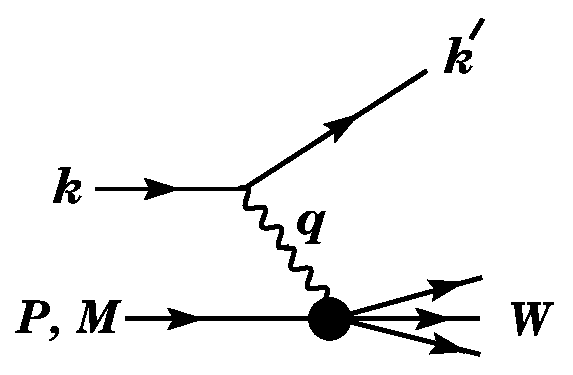
\includegraphics[width=0.8\linewidth]{intr/leptoprod.eps}
    \caption{轻子-核子散射过程示意图。}%
    \label{fig:leptoprod}
\end{figure}
电子-核子的非弹性散射过程$l N \to l X$如图\ref{fig:leptoprod}所示,
$k$和$k'$分别是入射和出射的电子的动量,通过
传播子$\gamma$, $W$或$Z$将动量$q=k-k'$传递给核子,
核子则蜕变为一簇强子。我们将
初态核子的动量记为$P$,末态强子的动量总和记为$W$。
实验上,$x$和$y$是经常被用到的无量纲的物理量,被称为Bjorken变量,
它们的定义为:
\begin{itemize}
    \item $x= \frac{Q^{2} }{2 M \nu}$,式中$Q^2 = - q^2$,
        $\nu$为电子和核子质心系下的能量损失。
        $x$物理意义为被撞的部分子携带的核子动量的比例。
    \item $y = \frac{q.P}{k.P} = \frac{\nu}{E}$,
        物理意义为电子在核子质心系下的能量损失比例。
\end{itemize}
    当$Q^{2} \gg M^{2}$时图示的过程为深度非弹性散射过程,其微分散射截面~\cite{Blumlein:1996vs,Forte:2001ph,Anselmino:1993tc}
的一般形式为
\begin{equation}
\frac{d^2 \sigma^i} {dx dy} 
    = \frac{4 \pi \alpha^2}{xy Q^2} \eta^{i}
    {(1-y - \frac{x^2 y^2 M^2}{Q^2}) F_{2}^{i}
+ y^2 x F_{1}^{i} \mp (y- \frac{y^2}{2}) x F_{3}^{i}
},
\end{equation}
\begin{figure}[htpb]
    \centering
    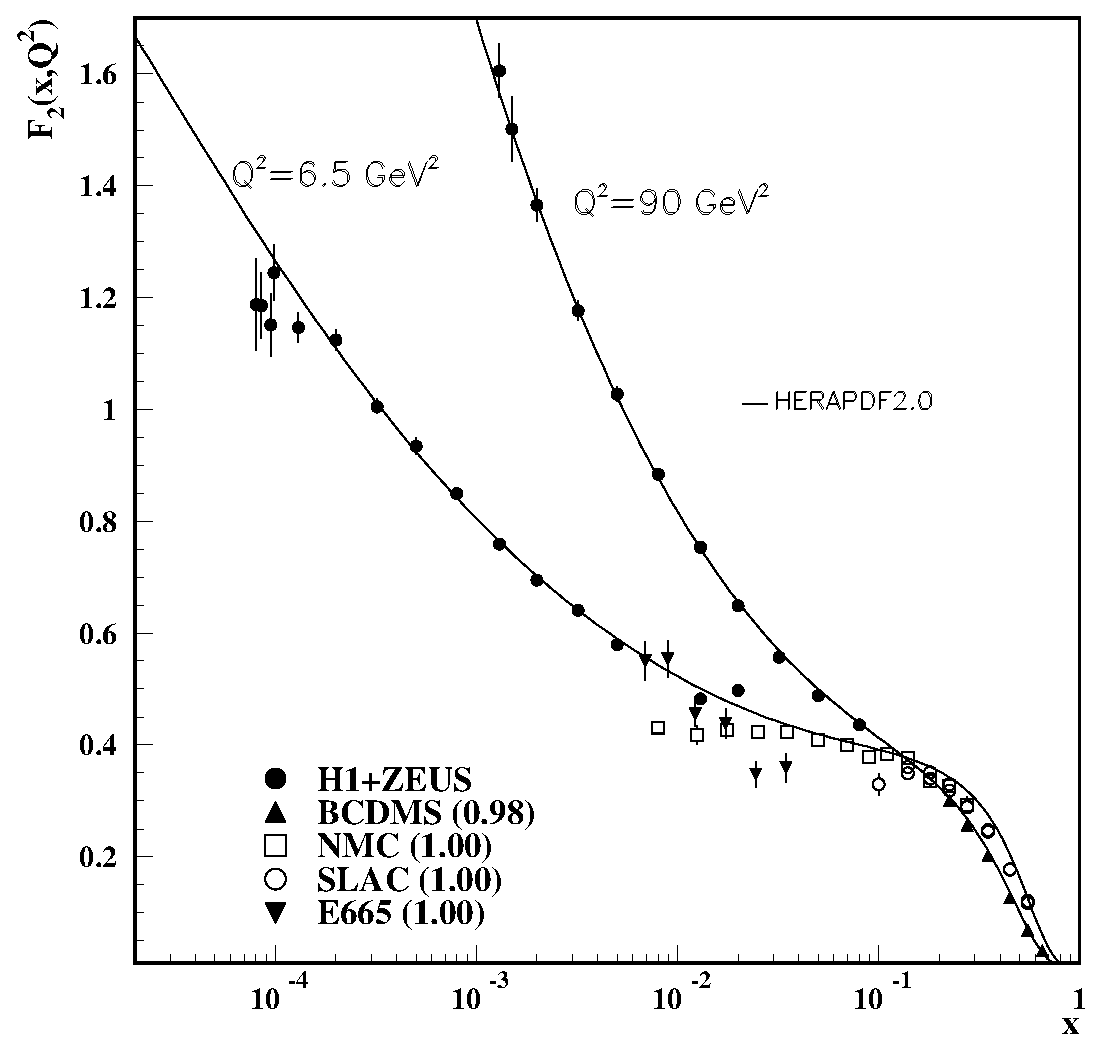
\includegraphics[width=0.8\linewidth]{intr/f2vsx.eps}
    \caption{结构函数的实验测量结果。}%
    \label{fig:f2vsx}
\end{figure}
和核子的内部结构紧密相关,一般的用形状因子$F(x, Q^2)$来描述。
图\ref{fig:f2vsx}展示了$F_{2}$的两组实验测量结果,分别
选取$Q^{2}=6.5,90$ GeV。$F_2$的相关定义见文献\cite{Klein:1983vs}
在$x$极小的区域,即$x<0.1$, $F_{2}$对$Q^2$的依赖较强,然而在$x$较大的区域,
即电子能量损失比较大时,$F_2$几乎不依赖与电子的入射能量,这意味着电子行为在一定程度上与其能量无关,
这就是所谓的标度无关现象。
标度无关的概念最早由James Daniel Bjorken提出\cite{Bjorken:1968dy}.
标度无关现象激起了当时对核子结构的热烈探讨,其中费曼提出的部分子模型(parton
model)是最著名也是最富有成效的,强有力的支持了夸克模型,这个由盖尔曼在1964年提出
的模型,这里的部分子就是盖尔曼模型中的夸克\cite{Greenberg:1981zv}。

图\ref{fig:fix_collider_kineplane}展示了各个实验所长,
\begin{figure}[htpb]
    \centering
    \includegraphics[width=0.8\linewidth]{intr/fix_collider_kineplane.eps}
    \caption{各个实验及能区。}%
    \label{fig:fix_collider_kineplane}
\end{figure}
将图\ref{fig:leptoprod}所示的过程旋转$90^{\circ}$就是另一种研究核子结构的实验手段,
即对撞机实验$e^{+} e^{-} \to N X$,其中最特殊的一种过程是$ e^+ e^- \to B \bar{B}$,
即末态是一对正反重子。
其中的一个打靶实验所不能的优势方面是能够研究超短寿命重子的结构函数,比如超子家族。
$\Lambda$是第一个被实验发现的超子,也是质量最轻的超子,如图所示,它留下的痕迹就是
一个``$\Lambda$``形状。在此之后,
重子八重态家族的其他成员$\Sigma$, $\Xi$, $\Omega$也陆续地被发现。
幸运的是所有的八重态重子都能在正负电子对撞机上成对产生,且产额可观,来源众多。
以BESIII为例,BESIII合作组在2009年和2012年间共取得了13亿的$J/\psi$
样本,主要的正反重子对的产额列举在表\ref{tab:bbar_production}中
 \begin{table}[htpb]
     \caption{BESIII上的正反重子对产额。只考虑$J/\psi$样本}%
     \label{tab:bbar_production}
     \centering
     \begin{tabular}{p{0.4\linewidth}
         p{0.25\linewidth}<{\centering}c
         p{0.25\linewidth}<{\centering}c }
         \toprule[0.2em]
         Decay mode & $\mathcal{B}(\times 10^{-3})$ & $N_{B} (\times
         10^{6})$ \\
         \midrule
         $J/\psi \to \Lambda \bar{\Lambda}$ & $1.61 \pm 0.15$ &
         $1.61 \pm 1.5$ \\
         $J/\psi \to \Sigma^{0} \bar{\Sigma}^{0}$ & $1.29 \pm 0.09$ &
         $12.9 \pm 0.9$ \\

         $J/\psi \to \Sigma^{+} \bar{\Sigma}^{-}$ & $1.50 \pm 0.24$ &
         $15.0 \pm 2.4$ \\

         $J/\psi \to \Xi^{-} \bar{\Xi}^{+}$ & $0.86 \pm 0.11$ &
         $8.6 \pm 1.0$ \\

         $J/\psi \to \Xi^{0} \bar{\Xi}^{0}$ & $1.20 \pm 0.24$ &
         $12.0 \pm 2.4$ \\
         $\psi(2S) \to \Omega \bar{\Omega} $ & $0.05 \pm 0.01$ &
         $0.15 \pm 0.03$ \\
         \bottomrule
     \end{tabular}
\end{table}
此时一个引人入胜的问题除了$c\bar{c}$共振态,正反重子对的产生是否还有其他来源?
一个备选的选项是奇异粲介子,
本文选定了标准模型允许的衰变过程$D_{s}^{+} \to p \bar{p} e^{+} \nu_{e}$
来寻找这种来源,相关的研究在后续的章节中有详细的描述。
另一个独特优势是借助于末态重子的极化信息能够获得更多的结构函数细节。
在$3.0~{\rm GeV}$能区,电子和超子的电磁相互作用起主导,
我们常用电磁形状因子$G_{E}(G_{M})$来称呼光子做传播子时的结构函数,此时的
散射类型为非弹性散射。一般的,散射振幅的形式为
\begin{equation}
    \begin{split}
        \frac{d\sigma}{d \cos\theta}  \sim & 1+ \alpha _{\psi } \cos^2\theta
        + \sin ^2\theta \hat{s}_{1}^x \hat{s}_{2}^x
        + \alpha_{\psi} \sin^2\theta \hat{s}_{1}^y \hat{s}_{2}^y 
        - \left( \alpha_{\psi} +\cos^2 \theta  \right)\hat{s}_{1}^z
        \hat{s}_{2}^z \\
        &+ \sqrt{1-\alpha_{\psi}^2} \cos\Phi  \sin\theta 
          \cos\theta
        \left( \hat{s}_{1}^x \hat{s}_{2}^z  - \hat{s}_{1}^z \hat{s}_{2}^x\right)
        +\sqrt{1-\alpha _{\psi}^2}
        \sin\Phi  \sin\theta \cos\theta  (\hat{s}_{1}^y - \hat{s}_{2}^y),
    \end{split}
    \label{eq:BBbar_amplitude}
\end{equation}
式中
\begin{equation}
    \alpha_{\psi} \equiv \frac{s |G_{M}|^{2} -4 m^{2} |G_{E}|^{2} }
    {s|G_{M}|^{2} + 4 m^{2}|G_{E}|^{2}},
\end{equation}
需要特别指出,只有当电磁形状因子$G_{E}$与$G_{M}$之间存在相位差时才能独立测量两个超子的衰变常数。
而末态超子的极化强度与相位差的正弦成正比,极化为
\begin{equation}
    P^{y}_{B} = \frac{\sqrt{1 - \alpha_{\psi}^{2}} \sin \Phi
    \sin \theta \cos \theta}
    {1+ \alpha_{\psi} \cos^{2} \theta}
\end{equation}
在 2018 年 BESIII 合作组\cite{Ablikim:2018zay}对 $J/\psi \to \Lambda \bar{\Lambda}$的事例进行拟合,
发现 $\Lambda$ 是部分极化的,观测到的极化强度随极角的分布为
\begin{figure}[htpb]
    \centering
    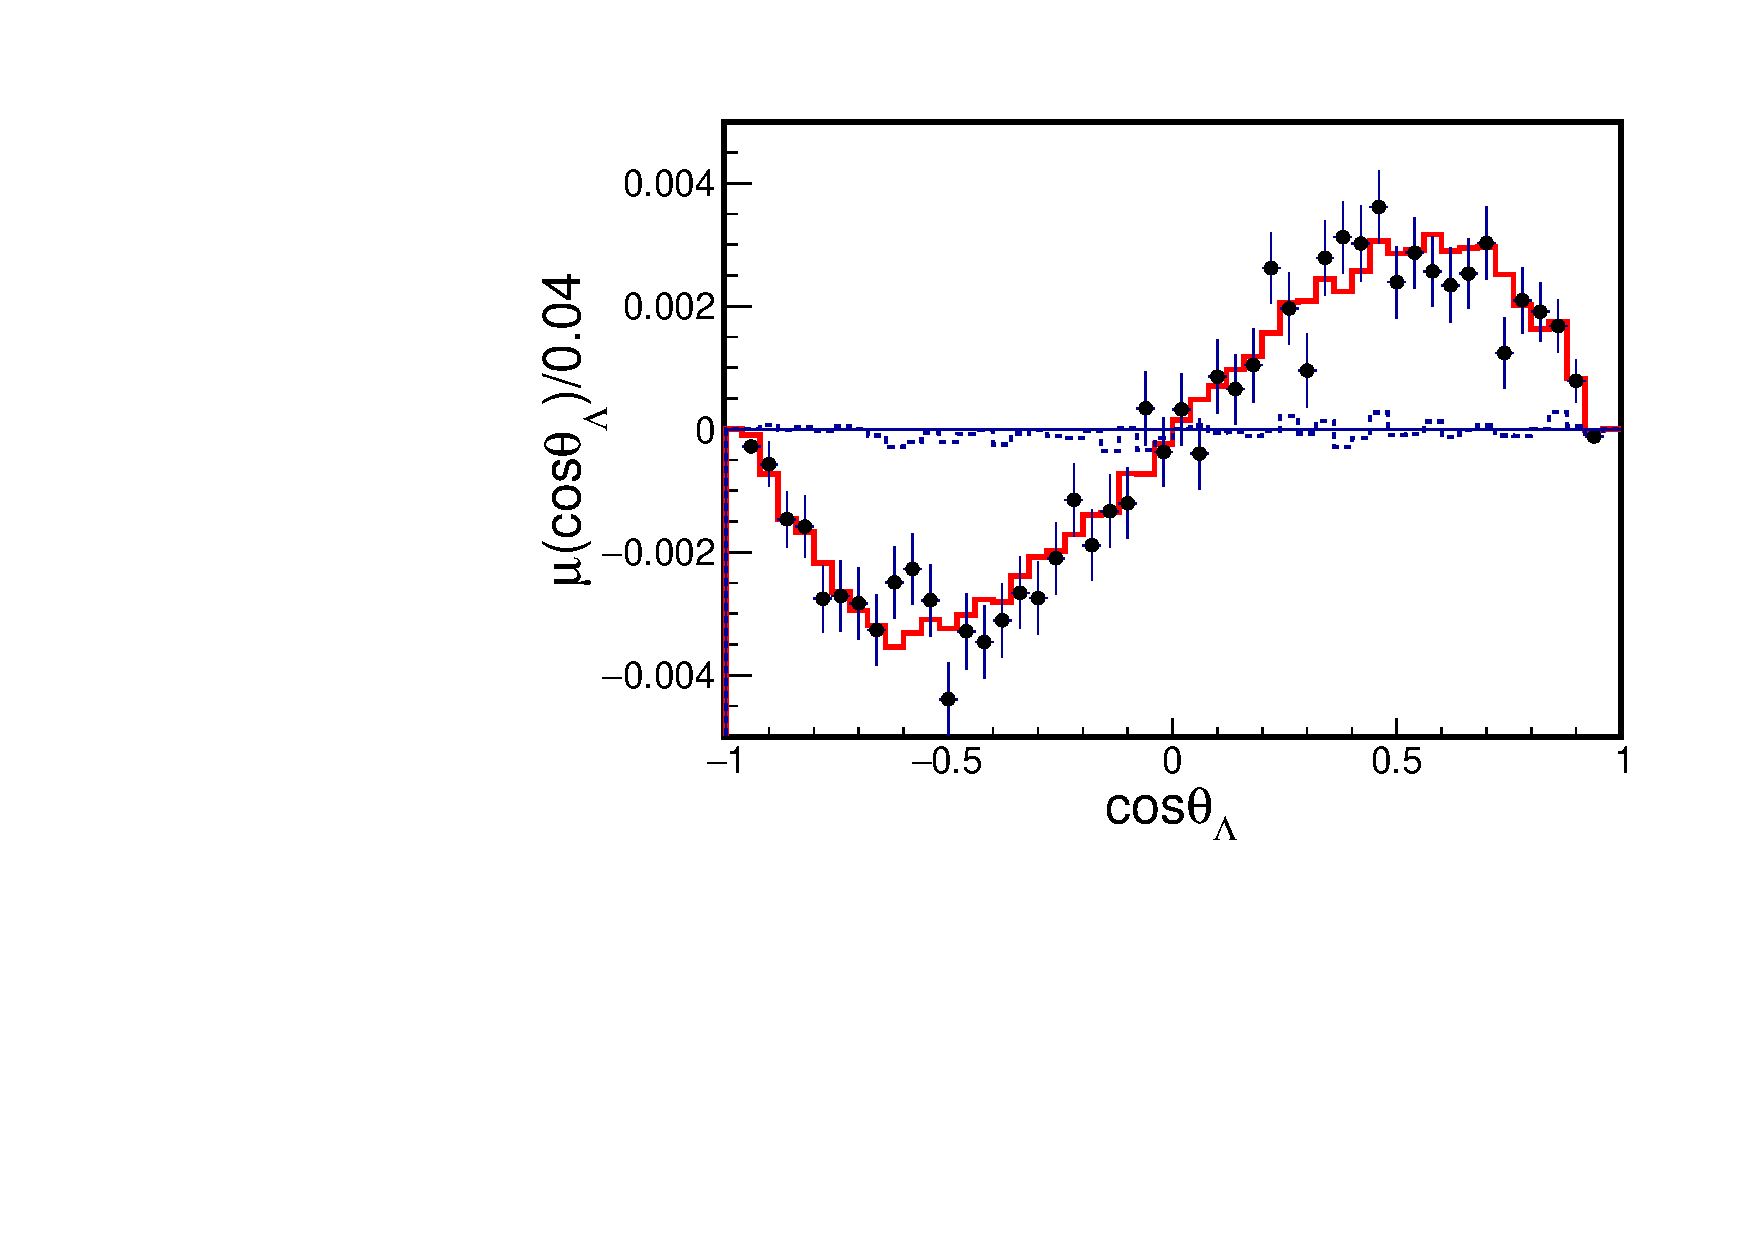
\includegraphics[width=0.9\linewidth]{intr/figPNa.pdf}
    \caption{末态$\Lambda$的极化强度随极角的变化而变化。}%
    \label{fig:figPNa}
\end{figure}
对八重态的成员进行一系列的研究迫切而重要,这也是本文选题动机的原因之一。
将图\ref{fig:leptoprod}中的入射轻子旋转$180$°则又一种研究结构函数的方式,即通过超子的衰变过程
$B' \to B l^{+} l^{-}$,这相应于$Q^{2}$极小的情形,即结构函数在零点时的行为。
一个理想的过程是$\Sigma^{0} \to \Lambda e^{+} e^{-}$,在几个超子的达利兹衰变中,
这个分支比最大,理论预期为$0.5\%$,这两项研究结合在以前将充分利用的对撞机产生的
$\Sigma^{0} \bar{\Sigma}^{0}$样本,这是本文选题的另一个重要原因。 
在接下来的章节里,将首先研究重子对的产生过程,包括粲介子中正反质子对的产生(第章),
$c\bar{c}$共振态$J/\psi$和$\psi(2S)$中$\Sigma^{0}\bar{\Sigma}^{0}$的产生,并详细的
测量了实验的衰变参数,包括$\alpha_{\psi}$,$\Delta \phi$, $\alpha_{\Lambda}$, $\alpha_{\bar{\Lambda}}$,
和$\alpha_{\gamma}$,并在此基础了谈论了在$\Sigma$衰变过程中的P、C和P宇称守恒
接着文章讨论了
磁场对实验测量的潜在影响并做了数值估计,最后本文研究了$\Sigma^{0}$的达利兹衰变过程
$\Sigma^{0} \to \Lambda e^{+} e^{-}$。




\chapter{北京谱仪实验}
\label{chap:bes3}

北京正负电子对撞机~(${\rm BEPC}$)~和相应的探测器北京谱仪~({BES})~于~{1988}~年~{10}~月
在中国科学院高能物理研究所建成。{1994}~年至~{1996}~年间,
对撞机和探测器进行了升级,升级后的对撞机仍称为~BEPC,探测器称为~BESII。升级后的对撞机和探测器的性能均有了很大的改进,取得了一系列在国际高能物理届有重要影响的研究成果,如~$\tau$~轻子质量的精确测量、$2 \sim 5 \gev$~的强子反应截面~(R~值)~的精确测量、粲夸克偶素衰变的系统研究等。2003~年底,国家批准了北京正负电子对撞机重大改造工程。该工程于~2004~年开始动工,2008~年竣工,2009~年通过国家验收并开始收集物理事例。升级后的对撞机和探测器分别称为~BEPCII~和~BESIII。至今为止,BESIII~已收集大量的实验数据,如表~\ref{tab:bes3data}~ 所示,并取得了丰硕的研究成果。

\begin{table}[!htb]
\centering
\small
\setlength{\abovecaptionskip}{0pt}
\setlength{\belowcaptionskip}{5pt}
\caption{BESIII~收集的实验数据简介。}
\begin{tabular}{lcc}
\toprule
数据样本 &  质心系能量~($\gev$) & 积分亮度或事例数 \\ \hline
$\jpsi$~数据 & $3.097$ & $1.3\times10^9$ \\
$\psip$~数据 & $3.686$ & $4.5\times10^8$ \\
    $\psipp$~数据 & $3.773$ & $2.9\,{\rm fb}^{-1}$ \\
    $\tau$~轻子质量扫描数据 & 3.554 & $24\,{\rm pb}^{-1}$ \\
    $XYZ$~数据 & 3.81$\sim$4.6 & $5\,{\rm fb}^{-1}$ \\
    $R$~值和~QCD~数据 & $2\sim3,\ 3.85\sim4.59$ & $0.5\,{\rm fb}^{-1},0.8\,\rm{fb}^{-1}$ \\
\bottomrule
\end{tabular}%
\label{tab:bes3data}
\end{table}

本章主要包括北京正负电子对撞机的简介、北京谱仪的物理目标和探测器结构以及北京谱仪的离线软件系统的介绍。

\section{北京正负电子对撞机}
BEPC~是工作在~$\tau$-粲能区的高亮度、多束团的正负电子对撞机~\cite{BEPCII},
而升级后的~BEPCII~的峰值亮度比它的前身还要高了两个量级。BEPCII~主要由注入器、束流输运线
和储存环构成。注入器是一台长度为~202\,m~的直线加速器,
由电子枪产生的电子以及由电子打靶产生的正电子一起被直线加速器加速后,
经由束流输运线注入到储存环中。储存环是一台环形的加速器,
正负电子束流在环内被累积、加速、储存和对撞。
BEPCII~在原有的储存环隧道的基础上采用双环方案,
使正负电子束流能够在两个彼此独立的储存环中累积、加速,并在对撞点处发生对撞。
双环结构是使束流亮度能够提高两个量级的关键\cite{BESIII-design}。
BEPCII~的主要性能参数可参见表~\ref{tab:BEPCII}。
值得一提的是,$2016$~年,BEPCII~的亮度达到了
$1 \times 10^{33} {\rm cm}^{-2} {\rm s}^{-1}$~的量级,
处于世界的前列。
此外,北京正负电子对撞机还实现了所谓的“一机两用”,
即在同步辐射模式下,可以作为光源以供物理研究。
\begin{table}
    \centering
    \small
    \setlength{\abovecaptionskip}{0pt}
    \setlength{\belowcaptionskip}{5pt}
    \caption{BEPCII的主要设计参数。}%
    \label{tab:BEPCII}
    \begin{tabular}{lc}
        \toprule
        束流能量~$E_{b}\,\gev$        & $1.0\sim2.3$  \\
        设计亮度~($E_{b}=1.89\,\gev$) & $1 \times 10^{33}\,{\rm cm}^{-2}{\rm s}^{-1}$ \\
    高频频率~(MHz)                & $499.8$ \\
    对撞周期~(ns)                 & $8$ \\
    储存环长度~(m)                & $237.53$ \\
    束团数目                      & $93$ \\
    正负电子注入速率~(mA/min)     & $50$ \\
    \bottomrule
\end{tabular}%
\end{table}

\begin{figure}
    \centering
    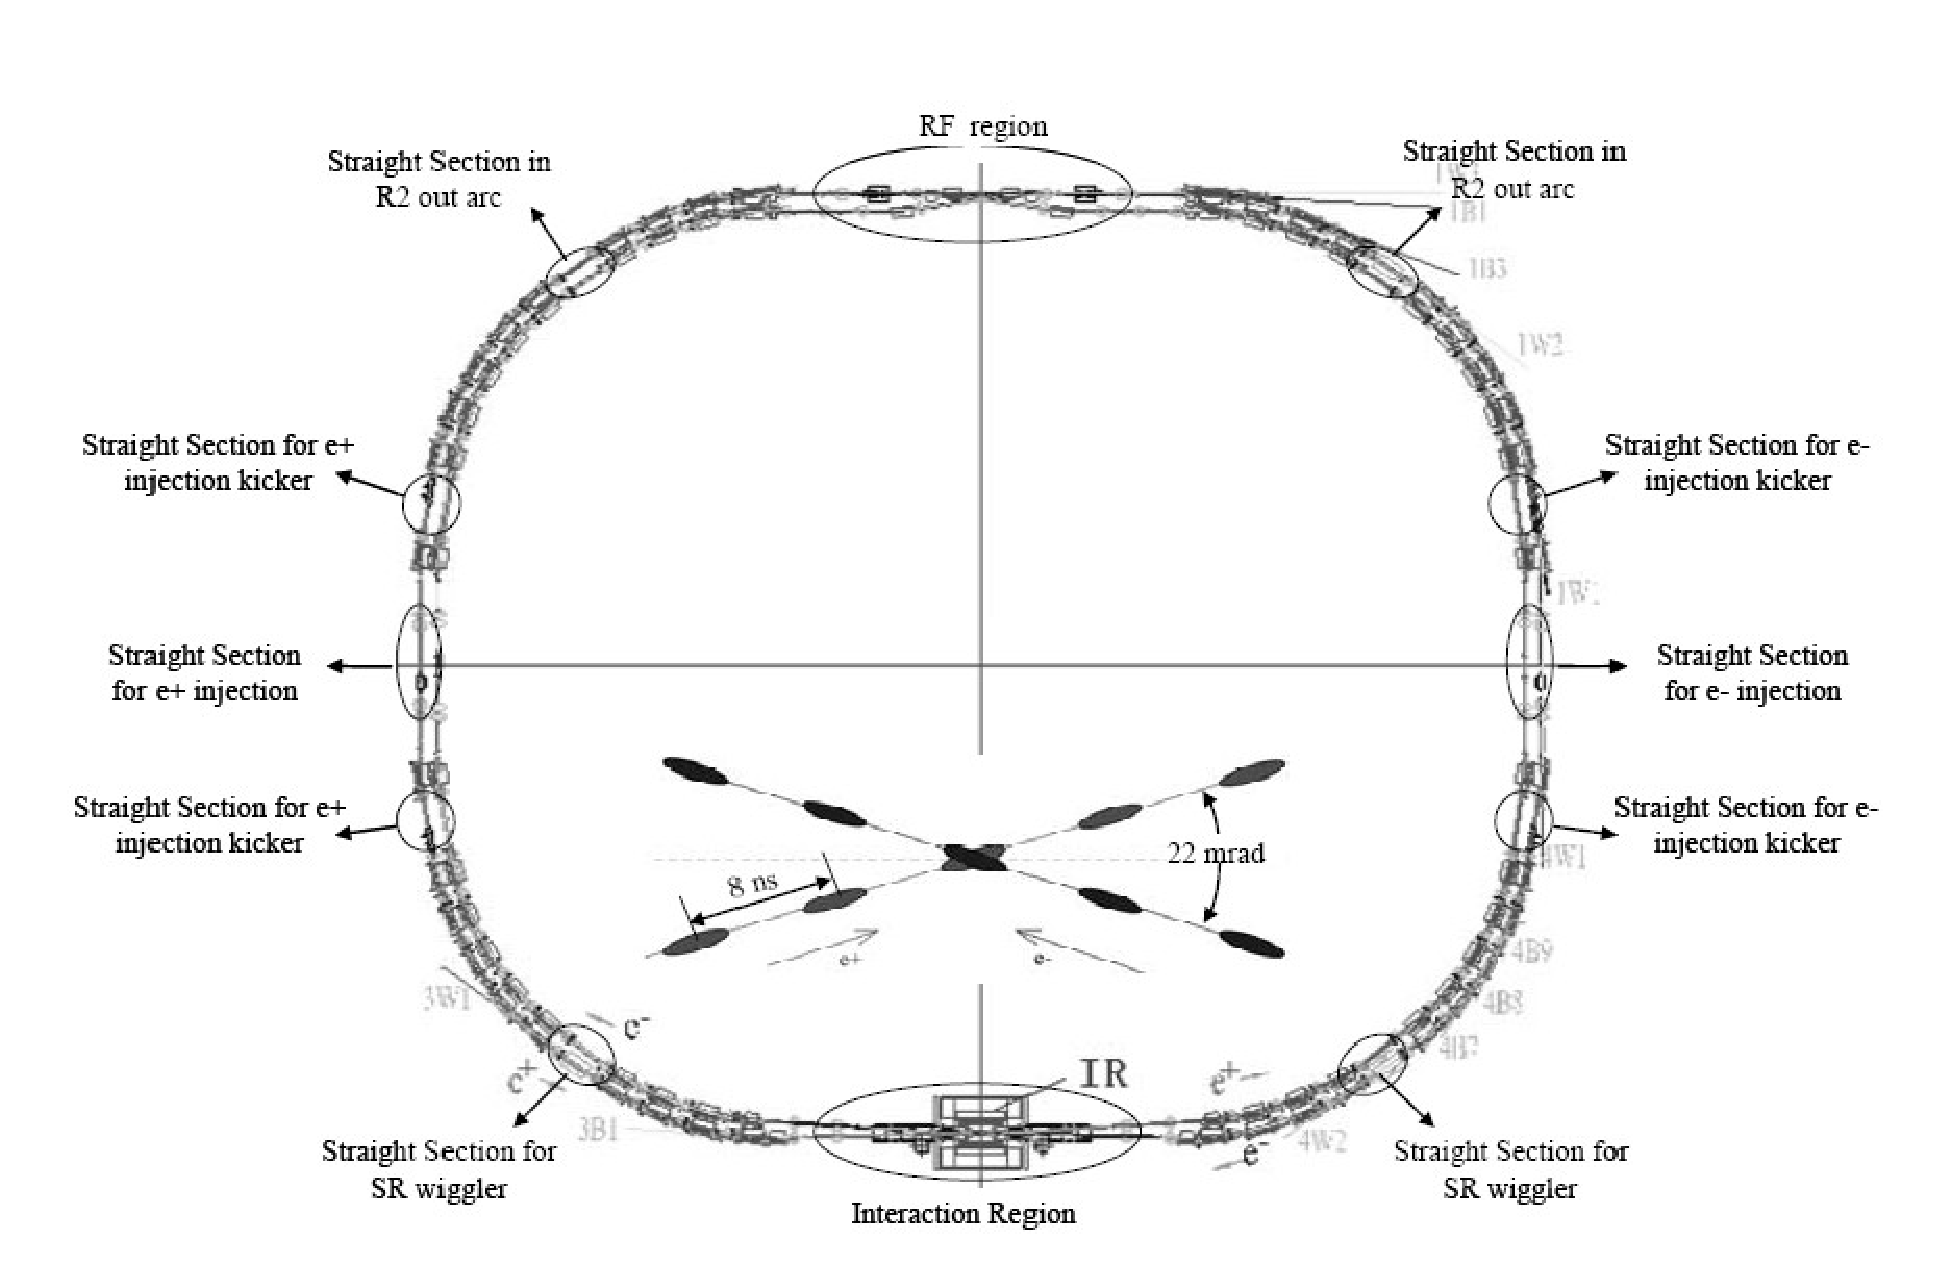
\includegraphics[width=0.8\textwidth]{bes3/BEPCII.eps}
    \caption{BEPCII俯视图。}%
    \label{fig:BEPCII}
\end{figure}

\section{北京谱仪}
BESIII~是运行在~BEPCII~上的工作于~$\tau$-粲能区的大型通用探测器~\cite{bes3},
其主要物理目标包括 $\tau$-粲能区的电、弱、强相互作用的研究以及新物理的寻找等
~\cite{bes3phys}。在收集了高统计量的数据的基础上,
BESIII~是用来精确检验标准模型和寻找新物理的理想场所。

BESIII~可以对电、弱相互作用理论提供精确的检验:通过对~$D$~和~$D_{s}$~介子衰变的精确测量来检验~CKM~(Cabibbo-Kobayashi-Maskawa)~\cite{CKM}~矩阵元的幺正性;通过对~$\tau$~轻子质量的精确测量来对轻子普适性提供更高精度的检验;通过对~$\tau^+\tau^-$~ 近域高精度的截面测量来加深对~$\tau^+\tau^-$~间相互作用的理解;利用~$\lcp\lcm$~阈值上的对撞数据,精确测量~$\lcp$~的各强子衰变以及半轻子衰变的性质。

由于强相互作用在~$\tau$-粲能区的非微扰性,使得目前在该能区的理论计算均具有
很大的不确定性。BESIII~利用~$\tau$-粲能区的数据对~QCD~展开了研究,
其中主要包括:结合高精度的~LQCD~的计算对标准模型的基本参数进行测量,
如强相互作用的耦合常数~$\alpha_{s}$~等;对低能强子谱进行研究,
寻找~QCD~预言的各种包含胶子的态,如胶球等;研究粲偶素的产生和衰变,
对量子色动力学提供精确检验。

BESIII~通过持续高亮度的运行,积累了大量的数据。
因而可以在~BESIII~上进行稀有衰变的寻找,如寻找味道改变中性流~(FCNC)~过程、
轻子数或重子数破坏的过程等。此外在标准模型中~$D^{0}-\bar{D^{0}}$~的混合
以及~$D_{s}$/$D$~衰变中的~$CP$~破坏效应都很小,而一些新物理模型可以加强
这种效应。在~BESIII~上利用高统计量的数据也可以对中性~$D$~介子的混合
及~$CP$~破坏进行寻找。

为了实现以上物理目标,BESIII~探测器需要满足的要求有:
\begin{itemize}
    \item 对光子进行精确测量,具有好的能量分辨、角度分辨以及识别能力;
    \item 对低动量带电径迹进行探测,精确测量其动量和角度信息;
    \item 好的粒子鉴别能力,能够对各种粒子进行区分,如电子、$\mu$~子、
        $\pi$~介子、$K$~介子和质子等;
    \item 好的前端电子学系统、触发系统和数据获取系统,适应~BEPCII~多束团模式
        下的高取数率,减少死时间。
\end{itemize}

根据以上的要求,BESIII~探测器的总体结构如图~\ref{fig:BESIII}~所示,
由内而外依次是主漂移室~(Main Drift Chamber, MDC)、
飞行时间计数器(Time-of-Flight, TOF)、
电磁量能器~(Electro-Magnetic Calorimeter, EMC)、
超导磁体~(Superconductor Magnet)~和~$\mu$~子计数器~(Muon Counter, MUC)。
BESIII探测器的主要性能参数~\cite{bes3}~可见表~\ref{tab:bes3p}。

\begin{figure}
 \centering
 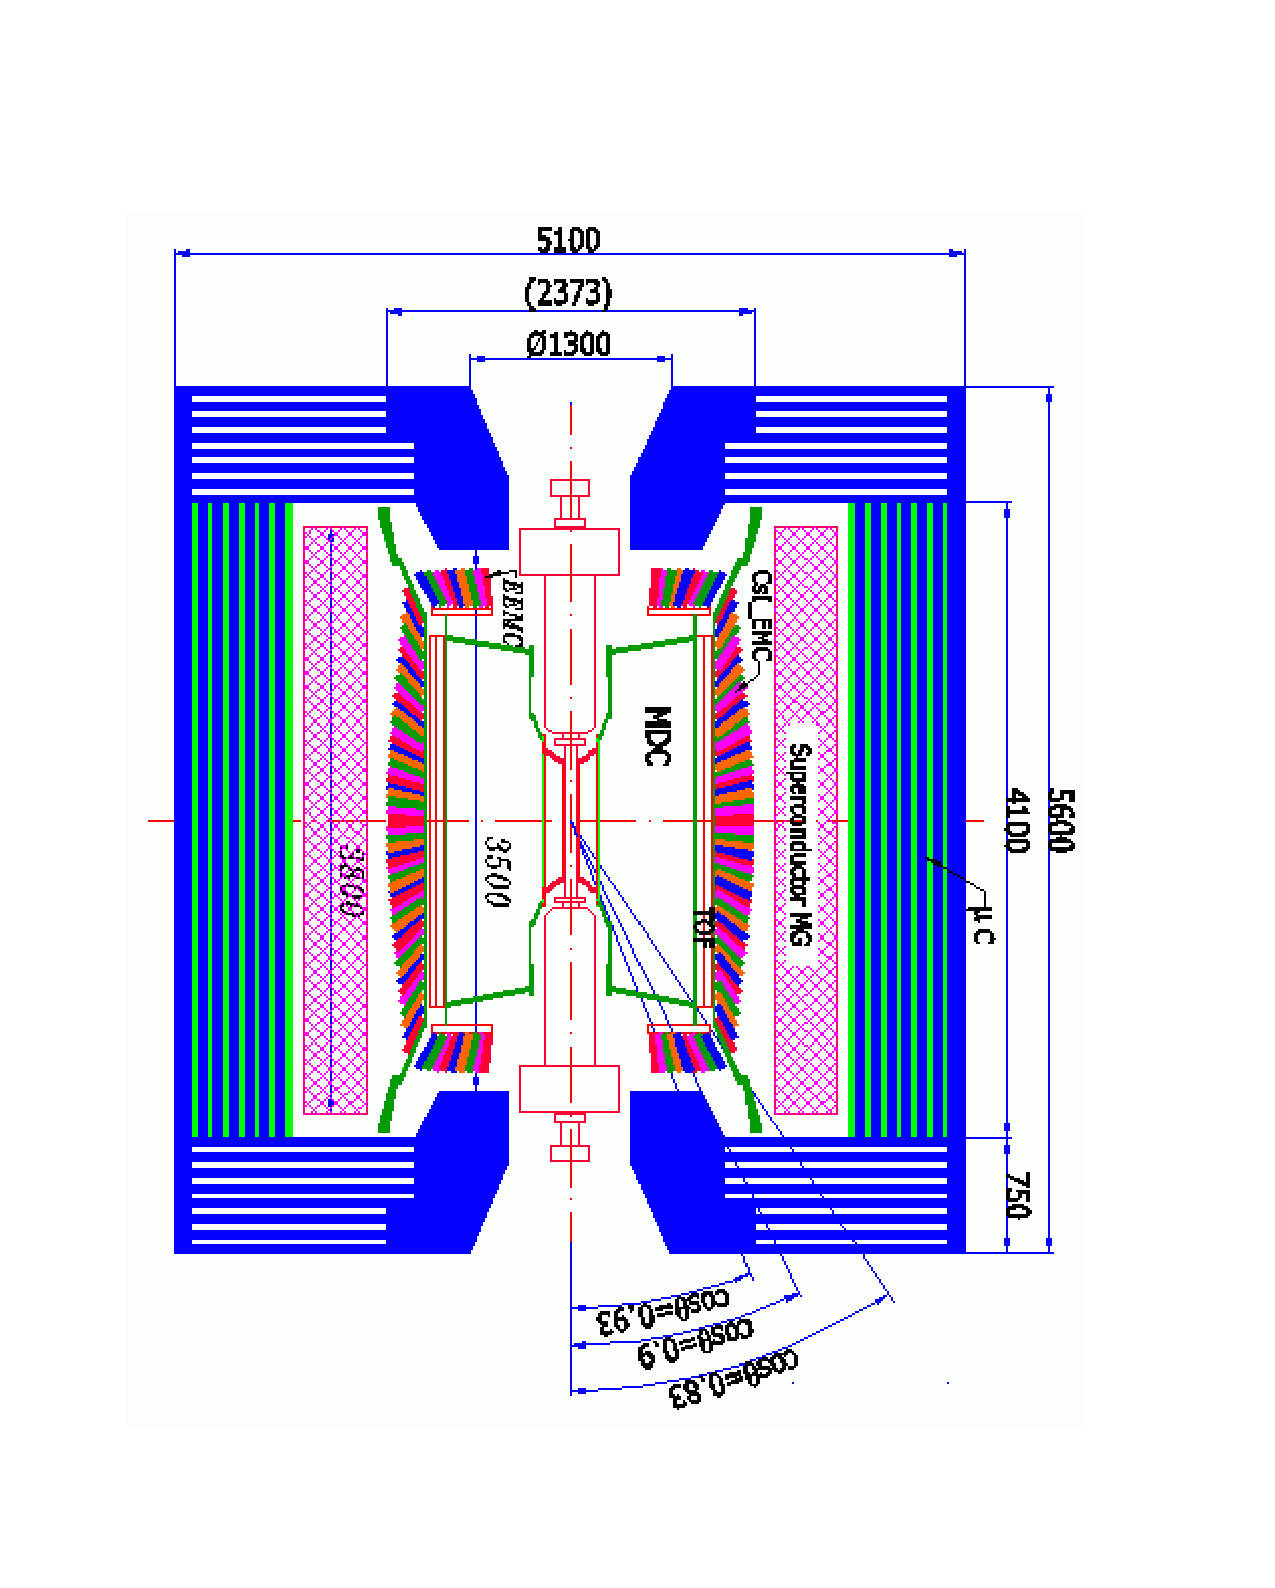
\includegraphics[angle=90,width=0.8\textwidth]{bes3/bes_view.eps}
 \caption{BESIII探测器的结构侧视图。}
 \label{fig:BESIII}
\end{figure}

\begin{table}
\centering
\footnotesize
\caption{BESIII主要性能参数。}
\begin{tabular}{ll}
\toprule
子系统                         & 主要性能参数 \\
\midrule
\multirow{3}* {主漂移室}       & $\sigma_{xy}$=130\ $\mu$m            \\
                               & $\Delta P$/{\it{P}}=0.5\ \% @1.0\ GeV     \\
                               & $\sigma_{dE/dx}$=6\ \%              \\
\midrule
\multirow{2}* {飞行时间计数器} &  $\sigma_{t}$= 100\ ps 桶部  \\
                               &  $\sigma_{t}$= 110\ ps 端盖  \\
\midrule
\multirow{2}* {电磁量能器}     &  $\sigma_{E}$/{\it{E}}=2.5\ \% @1.0\ GeV  \\
                               &  $\sigma_{\phi z}$=0.6\ cm  @1.0\ GeV  \\
\midrule
$\mu$ 子计数器                 &   9\ 层   \\
磁场强度                       &   1.0\ T \\
\bottomrule
\end{tabular}
\label{tab:bes3p}
\end{table}

\subsection{束流管}
束流管是储存环的一部分,它位于探测器的中心,分为中心束流管和外延束流管。其中中心束流管采用具有低原子序数且强度足够高的铍管,用来减小物质层的厚度,以减少多次散射对径迹动量分辨的影响。中心铍管采用了双层结构,中间为液态冷却系统,用来带走由粒子损失、同步辐射、次级粒子散射以及高频腔高次模产生的热量。两侧的外沿束流管由铜管或镀铜铝管制成,以减少因同步辐射产生的散射光子。

\subsection{主漂移室}
主漂移室是~BESIII~的最重要的子探测器,是一个与束流管相邻的圆柱形漂移室,
它的主要任务有:
1)~精确测量带电径迹的动量和方向;
2)~为带电径迹的粒子鉴别提供~$dE/dx$~信息;
3)~为带电径迹的一级硬件触发提供信号。
主漂移室采用了低质量材料,以及小单元的结构。考虑到对撞区的束流本底会
严重影响主漂移室的工作寿命,同时为了方便地安装束流管等部件,
主漂移室被设计成内室和外室两个部分。主漂移室沿径向一共有~43~层信号丝,
其中内室有~8~层,外室有~35~层。每~4~ 个信号丝层称为一个超层。
为了测量带电粒子的~$z$~坐标,内室的~2~个超层被设计为斜丝层,
其中第一个超层的斜丝相对于轴作负~$\phi$~方向的倾角排列,
第二个超层的斜丝为正~$\phi$~向的倾角排列。

BESIII~采用了强度为~1.0\,Tesla~的超导磁场。通过对带电粒子在磁场中的
飞行轨迹进行测量,从而计算出其动量大小和方向。
带电粒子在主漂移室内的工作气体中飞行时会发生电离,产生电子-离子对。
其中电子在电场的作用下会向信号丝漂移,正离子则向场丝漂移。
电子在漂移的过程中会发生雪崩放大,倍增后的电子被信号丝收集而产生电流,
这称为信号丝的一次着火。根据带电粒子在各层信号丝中留下的一连串的着火信息,
可以对其飞行轨迹进行测量。一般来说,飞行轨迹上的着火点越多,
动量的测量精度也就相应越高。 此外,根据~Bethe-Bloch~公式,
不同的带电粒子在同一工作气体中飞过单位路程所损失的能量~($dE/dx$)~是不同的,
如图~\ref{fig:dedx}~所示。通过对信号丝收集的电荷总量可以计算出粒子
的~$dE/dx$~信息,从而对粒子的类型进行鉴别。

带电粒子在主漂移室中飞行的过程中,会与探测器的物质层作用而发生多次库仑散射,
这将会对动量的测量精度造成影响。出于以上考虑,
主漂移室的工作气体使用氦气与丙烷的混合气体,场丝使用低原子序数的铝丝,
内室和外室的端面板也采用铝制材料,内、外桶采用炭纤维材料。
主漂移室的漂移单元采用小单元设计,如图~\ref{fig:mdc_danyuan_XT}~所示,
在每个小单元之中,信号丝位于中心,四周是接近方格分布的~8~或~9~根场丝。
主漂移室采用这种结构的优点是:
1)~减小粒子的漂移距离,缩短漂移时间,提供快速的触发信息,适合高计数率下的工作;
2)~减小电子扩散的贡献,获得更好的空间分辨;
3)~减少信号丝上的累积电荷,增长工作寿命;
4)~单元排列紧密,减少测量的死区,使~$dE/dx$~具有更好的分辨;
5)~ 具有多个测量单元,可以在有限的空间内提供更多的测量次数。
但是这种小单元结构也有一些不足:
1)~有些单元内电场分布不均匀,导致漂移距离和漂移时间的关系变复杂;
2)~单元边缘的电场会发生畸变,导致较强的边缘效应。
在一个小单元内,漂移距离~$X$~和漂移时间~$T$~的关系
可参见图~\ref{fig:mdc_danyuan_XT}。

内室的端面板被设计成小台阶形状,这种设计减小了端面板和内外室连接部件的变形。
外室的端面板包含了台阶部分和斜面部分。其中台阶部分的设计是为了满足
主漂移室的立体覆盖角达到~0.93\%$\times4\pi$,以及保证与束流管相连的
加速器的~Micro-$\beta$~聚焦磁铁的安放和电缆的引出有足够的空间。
斜面部分的设计,则是为了减小端面板在丝张力下的变形。
\begin{figure}
\begin{center}
 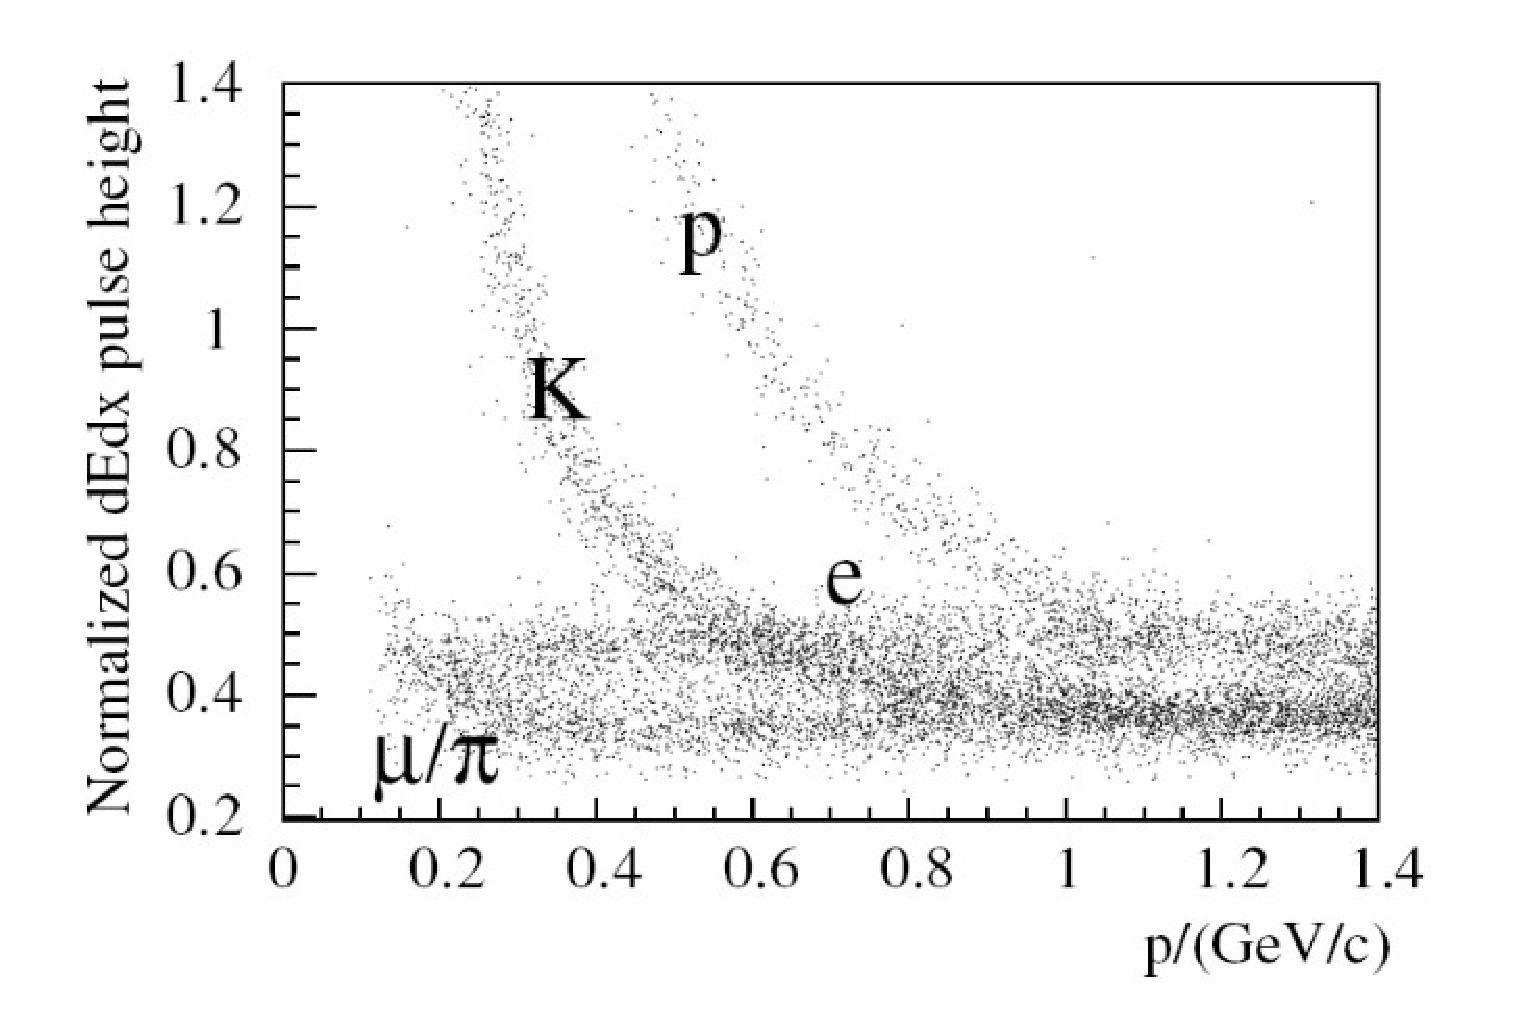
\includegraphics[width=0.55\textwidth]{bes3/dedx.eps}
 \caption{带电粒子的归一化脉冲高度~($dE/dx$)~随动量分布的散点图。}
 \label{fig:dedx}
 \end{center}
\end{figure}

\begin{figure}
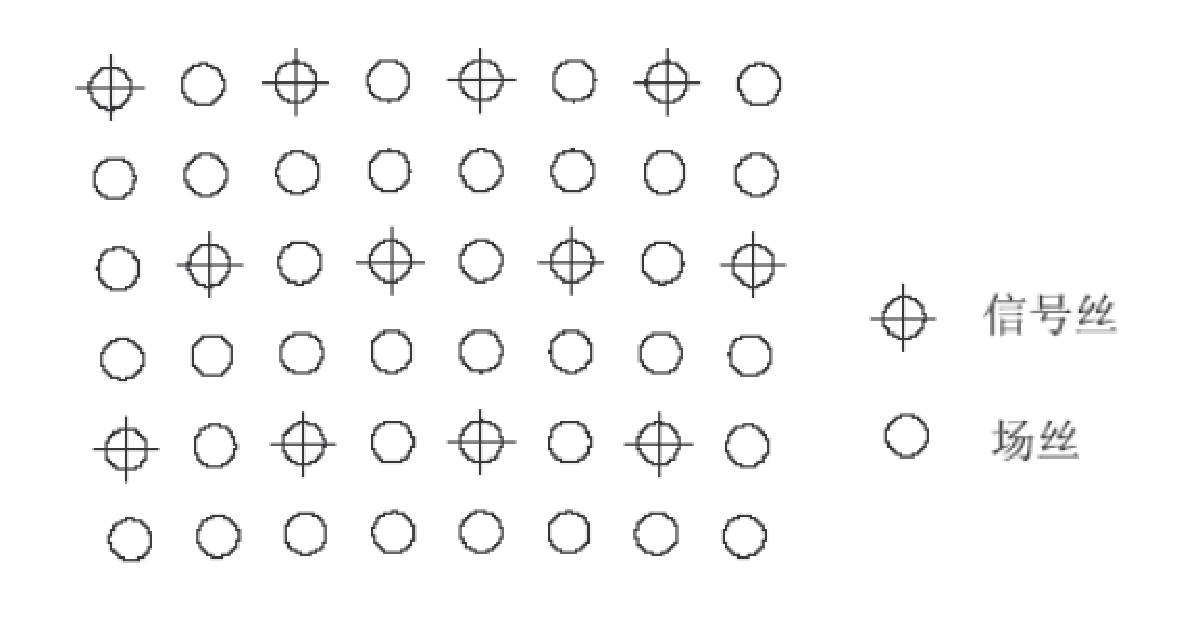
\includegraphics[width=0.5\textwidth]{bes3/mdc_danyuan.eps}
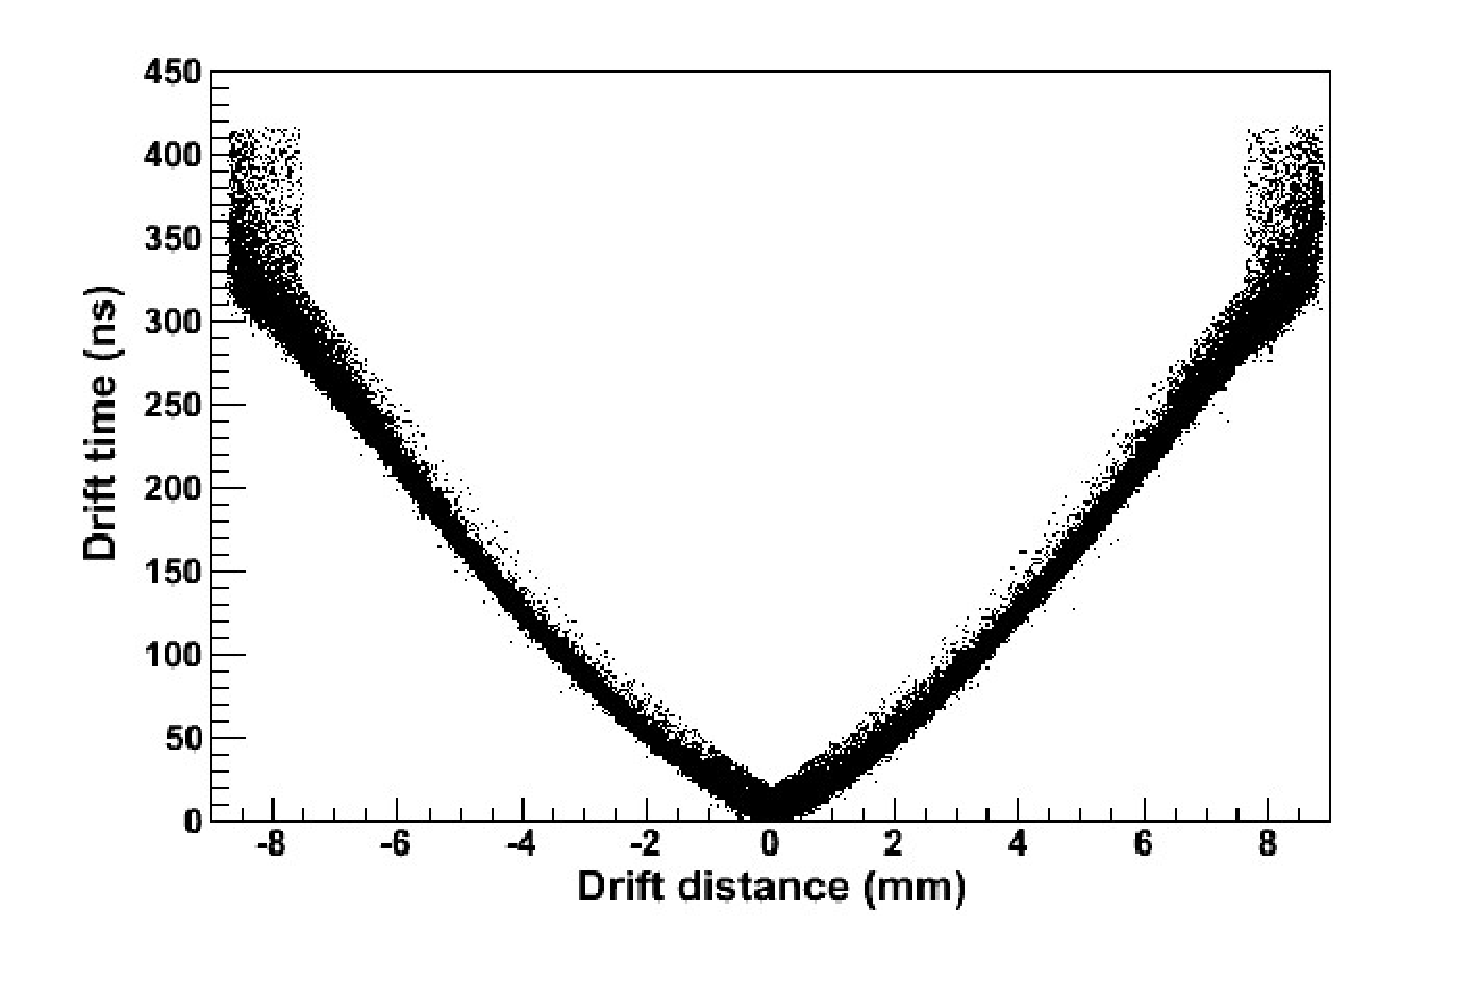
\includegraphics[width=0.4\textwidth]{bes3/X_T.eps}
\caption{漂移室的单元结构示意图(左)。漂移距离~$X$~和漂移时间~$T$~的关系(右)。}
\label{fig:mdc_danyuan_XT}
\end{figure}

\subsection{飞行时间计数器}
\label{subsection:tof}
飞行时间计数器的主要作用对飞行时间进行精确测量,并结合主漂移室测得的
粒子动量信息对粒子的种类进行鉴别。同时,飞行时间计数器还参与了初级触
发判选,利用不同探测器输出信号之间的时间信息排除来自宇宙线的本底。

飞行时间计数器位于主漂移室的外部,同样也分为桶部和端盖两部分。
其中桶部的接收立体角为~$82\%\times 4\pi$, 端盖的接收立体角
为~$10\%\times 4\pi$,$\cos\theta$~在~0.85$\sim$0.95~之间。
整个飞行时间计数器基本覆盖了主漂移室的接收度。飞行时间计数
器采用了塑料闪烁体作为探测元件,两端和光电倍增管连接在一起。
桶部采用了双层闪烁体结构,每个闪烁体具有两端读出,端盖采用
了单层结构,分为东西两部分,单端读出。桶部固定在主漂移室上,
端盖固定在电磁量能器上。桶部的设计分辨为~80$\sim$90\,ps, 
端盖的设计分辨为~80\,ps。在~$2\sigma$~鉴别能力的要求下,桶
部对于~$K/\pi$~的分辨可达到~0.9\,GeV/c。

飞行时间探测器主要由闪烁体、光导、光电倍增管和电子学四部分组成,
在~2015~年还在端盖部分安装了多隙阻性板探测器~(MRPC)。当高能带电
粒子穿过时,会与闪烁体发生作用,从而使闪烁体中的原子或分子电离而
损失能量。受激发的原子或分子在退激发过程中会发射光子,光子在闪烁
体内传播并由光阴极收集而发生光电效应,在光阴极上打出光电子,光电
子通过光电倍增管放大并被记录。

通过测量粒子的飞行时间,结合主漂移室测得动量和径迹信息,飞行时间
计数器可按照如下原理对粒子种类进行鉴别。
一个带电粒子的质量~$m$~和速度~($c \beta$)~应满足如下公式
\begin{equation}
\beta c  = \frac{L}{t_{tof}},\ m^2 = p^2 \times \frac{1-\beta^2} {\beta^2c^2},
\label{eq:mp}
\end{equation}
其中~$c$~表示光速,$L$~为飞行距离,$t_{tof}$~为粒子的飞行
时间,$p$~是粒子的动量大小。
从公式~(\ref{eq:mp})~我们可以看出粒子的飞行时间与其质量相关,
我们据此可以判断其粒子类型。

我们假定粒子的类型为~$i$,然后利用以下公式计算出其预期飞行时间:
\begin{equation}
t^i_{exp} = L  \sqrt{(\frac{m_i}{p})^2 + 1 },
\end{equation}
然后定义预期的飞行时间~$t^i_{exp}$~和与测得的飞行时间~$t_{tof}$~的
偏差为~$\chi_{TOF}^i$,$\chi_{TOF}^i$~的绝对值越小,粒子为~$i$~的概率越大。

\subsection{电磁量能器}
\label{subsection:emc}
电磁量能器是采用了~CsI~(T1)~晶体制成,而且同样由桶部和端盖两部分组成。
其桶部的内半径为~94\,cm,内长~275\,cm;端盖内半径为~50\,cm,距离对撞
点~Z=$\pm$138\,cm。
桶部共有~44~圈,每圈~120~块晶体。除第一圈外,对撞中心处~$\theta$~向的
左右两部分的晶体均指向距对撞中心~$\pm5$\,cm~的点,每层晶体在~$\phi$~向
相对于中心线有~$1.5\,^{\circ}$~的偏移。
端盖量能器由半圆环组成,在径向共有~6~层晶体结构,每层晶体均指向距对撞中
心~$\pm$10\,cm~的点。

电磁量能器主要用途是精确测量光子或带电粒子产生的电磁簇射,
确定光子的能量和位置信息,并提供中性径迹事例的触发。其工作
原理是:入射光子在物质原子核的库仑场作用下转化成正负电子对,
所产生的正负电子对又进一步发生级联韧致辐射和光子电子对转化。
直到所产生的的光子的能量低于光子转换成电子对的阈值能量时,
簇射过程停止。正负电子对可以激发出晶体能带中的电子--空穴对,
电子--空穴对复合后发出的光被硅光二极管吸收。通过硅光二极管收
集到的光的能量,可以测得到最初的入射粒子能量。

由于韧致辐射的功率与粒子质量的平方成反比,对于~$\gamma$~和
电子而言,在量能器中的辐射长度很短,几乎沉积了所有能量。而
对于其它带电粒子,则辐射长度较长,它们大多只在量能器中沉积
一部分的能量。因此可以利用带电径迹在量能器中的能量沉积与主
漂移室测得的径迹动量的比值~($E/p$)~来把电子和其他粒子鉴别开来。

\subsection{超导磁体}
超导磁体系统的主要用途是为主漂移室提供高强度的均匀稳定的轴向磁场,
用来使带电粒子发生偏转。它由超导线圈、直线电源、真空系统、低温系统
以及磁测系统组成,是BESIII的关键部件之一。磁感应强度的大小有以下考虑:
一方面较高的磁感应强度可以提高粒子动量的分辨,但另一方面过高的磁场也
会对低动量的径迹造成测量的困难。综合以上考虑,超导磁体系统采用由纯铝
为稳定体的~NiTi/Cu~合金缠绕而成的超导磁铁,由液氦作冷却剂,
并使用轭铁~(即~$\mu$~子鉴别器的吸收体)~ 提供磁场回路。超导磁体系统为
漂移室提供了约~1.0\,T~左右的轴向磁场,均匀度为~5\,\%,磁场的测量精度
可达到~0.1\,\%。

\subsection{$\mu$~子鉴别器}
$\mu$~子鉴别器~($\mu$ Chamber)~位于~BESIII~探测器的最外层,包括
由阻性板室~(RPC)~组成的~$\mu$~子鉴别器以及有夹层的轭铁组成的强子
吸收体,工作气体为~$\rm Ar/C_{2}H_{2}F_{4}/iC_{4}H_{10}(50/42/8)$
~混合气。其主要功能是鉴别反应末态中的~$\mu$~子,通过对多层击中点的
位置进行测量来确定粒子的飞行轨迹,再与内层探测器测量的径迹相匹配,
从而鉴别出~$\mu$~子,尤其是区分~$\mu$子~和~$\pi$~介子。

\subsection{触发判选系统}
BEPCII~采用的是多束团、高流强的对撞模式,这种模式极大程度地提高
了对撞亮度,但同时也给~BESIII~探测器带来了很高的本底,从而给后续
的电子学系统、触发判选系统、在线数据获取系统带来了挑战。其中触发
判选系统是快速实时的事例选择和控制系统,该系统需要把~BESIII~收集
的事例率压缩到在线数据获取系统可以接受的程度,并尽可能减少好事例的丢失。

BEPCII~的多个束团间的时间间隔一般为~8\,ns。触发判选系统无法在两次
对撞之间完成一次判选,我们要求触发和电子学系统使用流水线~(Pipe-Line)~
的方式对数据进行缓存与挑选。前端电子学可以缓存一段时间~(6.4\,$\mu$s)~
内的数据,触发判选系统需要在这段时间内完成初级硬件触发,给出触发信号~L1。
没有通过硬件触发的信息将被覆盖或丢弃。

\subsection{数据获取系统}
BESIII~的在线数据获取系统是基于前端电子学系统和触发判选系统的硬件系统,
它由读出系统、在线系统、慢控制系统、校准系统及其它服务系统组成。

数据获取系统的主要用途是收集经过初级触发判选的事例数据,
通过两级计算机的预处理和高速网络传输,将分布在各读出机箱中
的事例数据迅速汇集到在线计算机系统上,然后对事例进行包装和过滤,
组装成完整有效的事例,最终将事例数据标记并记录到永久的存储介质上。
数据获取系统使用了先进的计算机和网络技术,并采用了多级并行的处理方案;
为了从前端电子学系统中快速读出大量数据并尽可能减少系统的死时间,
大量采用了多级数据缓冲技术、并行处理技术、VME~总线高速读出技术及网络传输技术。

\section{离线软件系统}
BESIII~的离线软件系统~(BesIII Offline Software System, BOSS)~由主框架系统、
数据刻度系统、事例重建系统、事例模拟系统、实用软件包系统以及用户分析软件包
组成。其主要用途是对实验数据和蒙特卡洛~(Monte Carlo, MC)~\,\cite{mcsim}~
模拟数据进行处理,并对多种工具库和文件库进行管理。

\subsection{离线软件框架}
BOSS~是基于Gaudi框架,使用~C++~语言和面向对象的技术进行开发的,
它为数据刻度、事例重建、蒙特卡洛模拟及物理分析提供了统一的平台。
BOSS~框架结构以瞬态数据库~(Transient Data)~为核心;
对数据的存储和处理相对独立;提供了标准的用户程序嵌入点;
模块之间的操作通过标准的接口进行;对宿存~(Persistency)~数据和
瞬态数据进行独立管理;模块的开发遵循尽可能重用的原则。
BOSS~框架的主要组成部分为:算法模块~(Algorithm),应用
管理器模块~(Application Manager),瞬态数据库模块~(Transient Data Store),
服务模块~(Service)和转换器模块~(Converters)~等。

\subsection{探测器模拟系统}
蒙特卡洛方法是用来处理随机过程的一种有效方法。在高能物理实验中,通常要靠蒙特卡洛方法估计某个物理过程的探测效率。所以通过蒙特卡洛模拟产生的过程和要尽可能与真实过程一致。在~BESIII~上,这一过程由~(BESIII
Object Oriented Simulation Tool, BOOST)~来完成。BOOST~\cite{BOOST}~是基于高能物理实验中广泛应用的~Geant4~\cite{Ablikim:2009aa}~来开发的面向对象的框架系统,它包括物理事例的产生子、物质与几何结构的描述、磁场的描述、粒子与物质的相互作用、探测器的响应、真实化信息、数据输出和用户界面等部分。事例产生子以~HepEvt~的格式来产生物理事例,然后作为输入提供给~Geant4,接着由~Geant4~来构造探测器并模拟粒子在物质中的相互作用,同时记录下粒子在探测器中的响应信息。模拟系统采用基于~XML~(eXtensible Markup Language)~的统一几何描述标识语言--GDML~(Geometry Description Markup Language)~来构造~BESIII~各个子探测器的物质和几何结构。探测器的响应是独立于~Geant4~的,它利用粒子的击中信息来确定探测器的输出信号,这个过程也称为数字化过程~(Digitization)。探测器的击中信息在经过数字化后得到原始数据~(raw data),同时在模拟阶段也需要记录下模拟时粒子的真实信息~(MC truth)~以供重建和分析时使用。我们通过后期调试~(MC tuning)~ 来减小蒙特卡洛模拟与真实数据的细微差异,蒙特卡洛模拟的好坏直接影响了物理分析的精度。

事例产生子模拟了各种物理过程,根据反应机制和微分截面来生成物理事例,
并计算出初末态所有粒子的四动量信息。BESIII~模拟系统包括了~30~多个产生子,
如均匀相空间的产生子~(howl), $J/\psi\rightarrow\rho\pi$~事例产生
子~(rhopi)、$J/\psi$ 和$\psi(2S)$~单举衰变产生子~(lundcharm)等等。
这些产生子都是在不断完善中的,有时还需要用户根据自己的需求写出相应的产生子。

\subsection{离线重建系统}
BESIII~离线重建系统是~BESIII~离线软件系统的重要组成部分,
它负责利用~BESIII~各个子探测器收集的原始信息来得到末态粒子
的电荷、飞行轨迹、动量大小等感兴趣的物理信息,以供给后续的
物理分析使用。如图~\ref{fig:rec_flow}~所示,BESIII~离线重建
大致包括~MDC、TOF、EMC、MUC~等子探测器的重建和物理事例顶点的
重建~(一般一个~run~对应重建出一个对撞顶点)。其中~MDC~的重建
又包括事例起始时间的重建、MDC~主重建、$dE/dx$~重建、径迹
的Kalman~拟合和径迹的外推等等。
从下图我们可以看出事例起始时间的重建是在整个离线重建系统的最前
沿,直接影响着后续各个系统的重建质量。
\begin{figure}
\begin{center}
 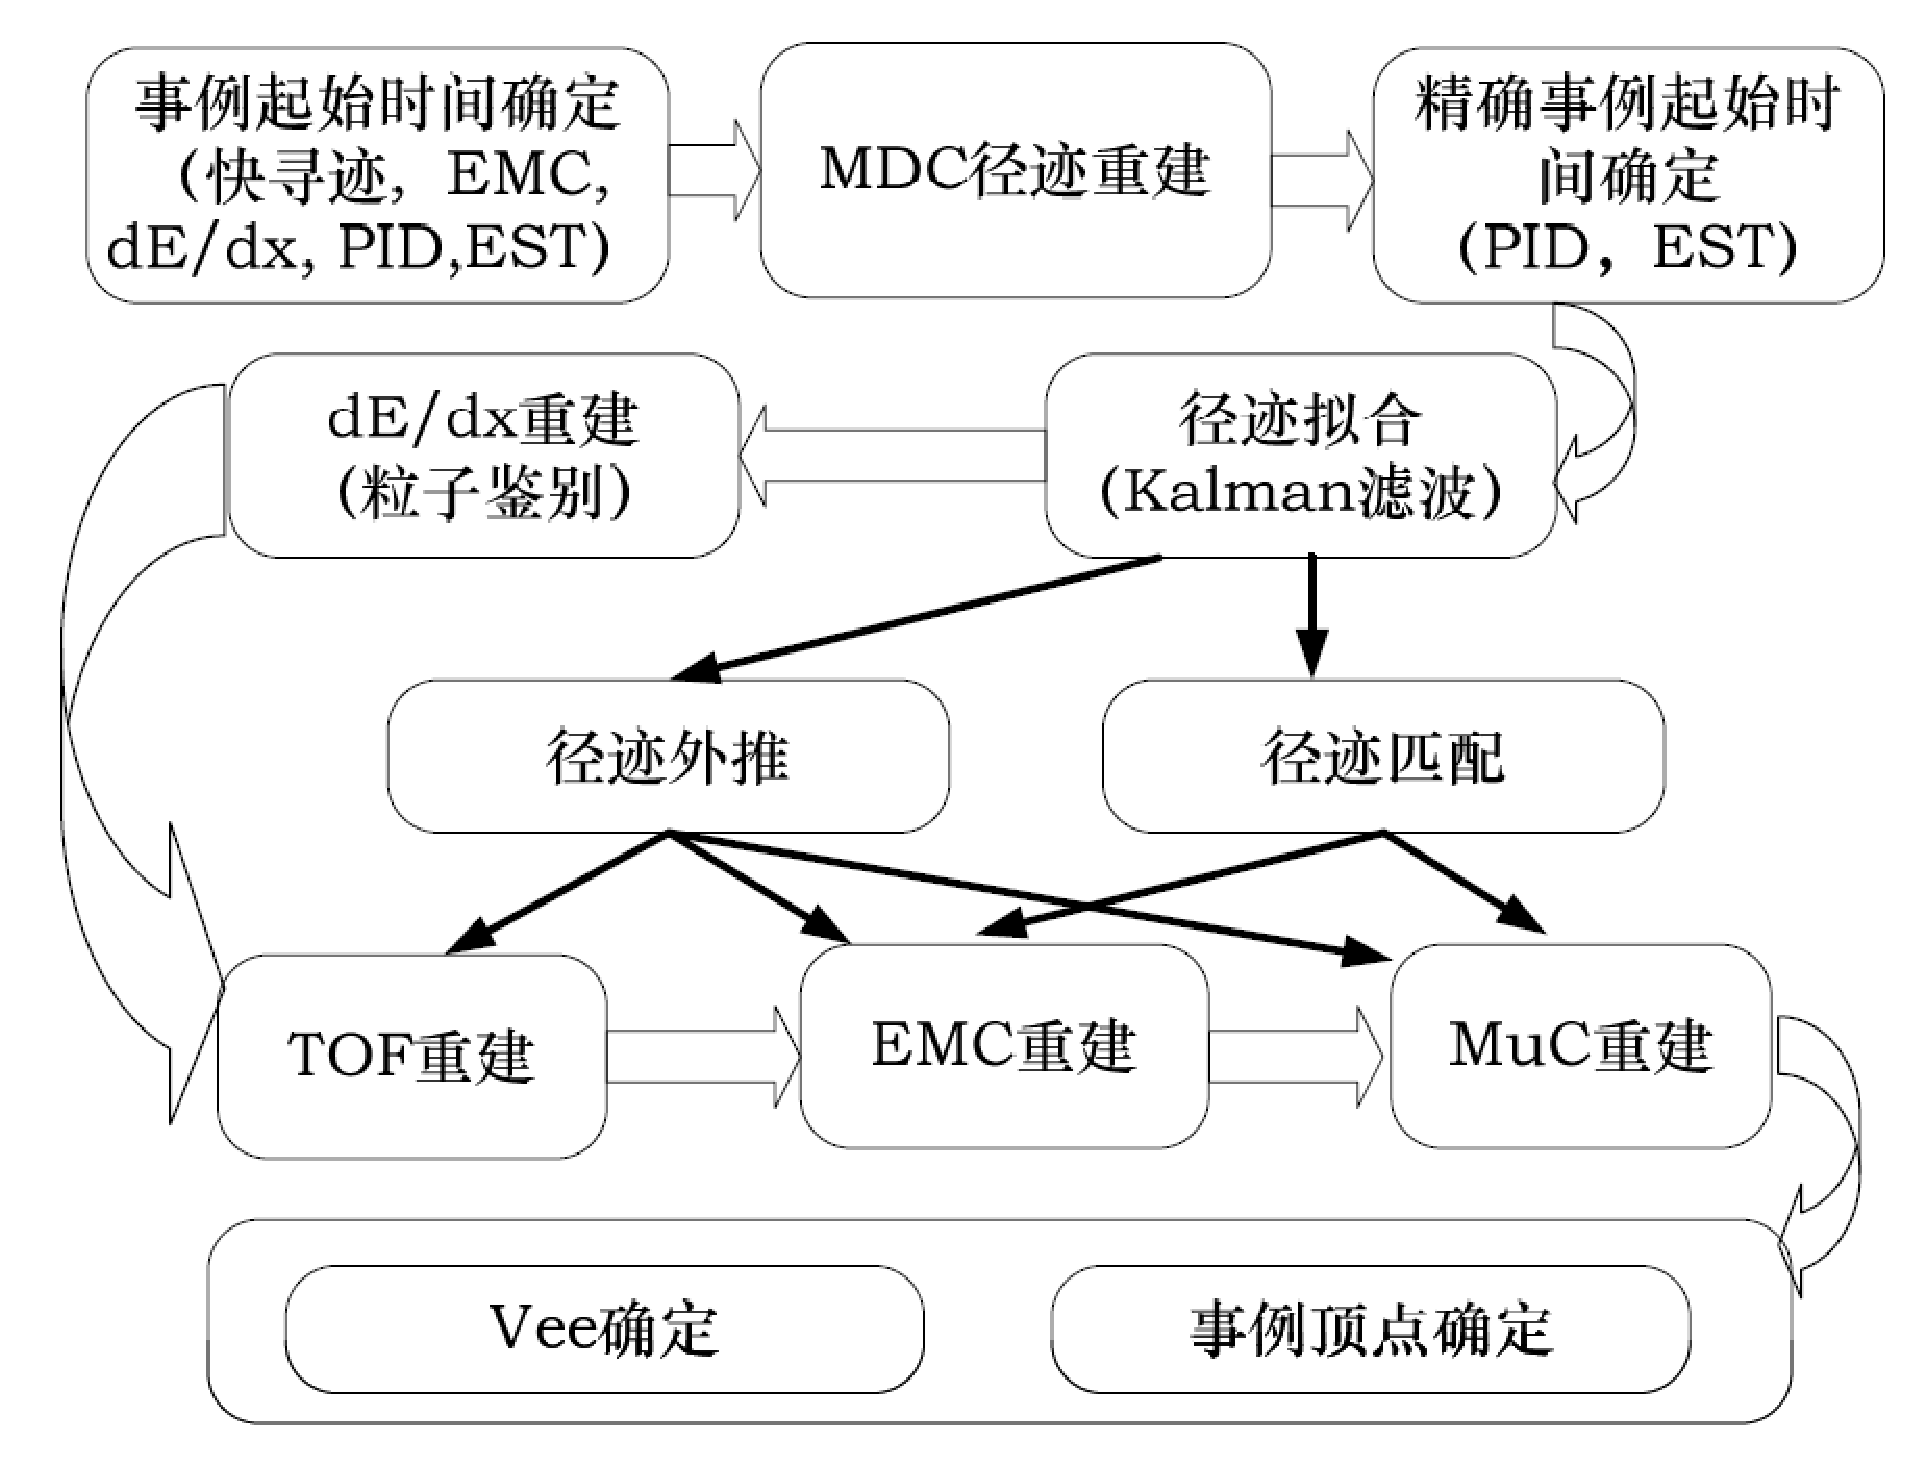
\includegraphics[width=0.65\textwidth]{bes3/rec_flow.eps}
 \caption{BESIII~的离线重建流程。}
 \label{fig:rec_flow}
 \end{center}
\end{figure}

\subsection{离线刻度系统}
正如前所述,末态粒子在各子探测器中留下的信息一般是以信号幅
度~(ADC)~和时间~(TDC)~的形式被记录下来的,但是各个子探测器
的工作状态并不是恒定不变的,同一子探测器的各部分相应也不一定均匀,
因入射粒子的角度不同探测器的响应也有所不同。因此必须有一套
能够精确反映各子探测器响应状态的参数,这套参数就是刻度常数。
离线刻度系统的任务就是获得这些刻度常数并对原始数据作系统的修正,
从而使测得的物理量更加准确。

\subsection{物理分析工具}
物理分析工具是一些为物理分析提供服务的公用的算法和接口。
BESIII~中的物理分析工具包括运动学拟合~(Kinematic Fitting)
~\cite{Yan:2010zze}、顶点拟合~(Vertex Fitting)、粒子鉴别~
(Particle Identification,PID)~\cite{Gang_2008}~和
事例组装~(Event Assembly)、亮度测量~(Luminosity Measurements)~
和分波分析~(Partial Wave Analysis,PWA)~等分析软件包。
这些软件能很好地提高物理分析的效率。

\section{本章小节}
本章介绍了BEPCII和BESIII的结构、BESIII 各个子系统的结构性能和共作原理等,
以及BESIII上的在线数据获取系统和离线软件系统。



% ====================================================
%   Copyright (C)2019 All rights reserved.
%
%   Author        : Xin-Xin Ma
%   Email         : xxmawhu@163.com
%   File Name     : ds_to_ppbarenu.tex
%   Last Modified : 2019-12-25 20:33
%   Describe      :
%
% ====================================================%
\chapter{寻找奇异粲介子的稀有衰变过程$D_{s}^{+} \to p \bar{p} e^{+} \nu_{e}$}%
\label{cha:ds_ppbarenu}
本章讨论的是在BESIII寻找$D_{s}^{+}$的稀有衰变$D_{s}^{+} \to p \bar{p}
e^{+} \nu_{e}$。
受相空间的限制,$D^{+}$和$D^{0}$均不能衰变到重子对。只有Ds可能
通过三种衰变方式产生重子对,它们分别是
\begin{align}
    D_{s}^{+} &\to p \bar{n} \\
    D_{s}^{+} &\to p \bar{p} e^{+} \nu_{e} \\
    D_{s}^{+} &\to n \bar{n} e^{+} \nu_{e}
\end{align}
前者被CLEOc首先发现~\cite{Athar:2008ug},分支比的实验结果为$(1.30 \pm
0.4)\times 10^{-3}$, 随后被BESIII加以确实\cite{Ablikim:2018iad},
分支比的测量精度得到了提高,实验结果为
$\mathcal{B}(D_{s}^{+} \to p \bar{p} e^{+} \nu_e) = (1.21 \pm 0.10 \pm
0.05)\times 10^{-3}$,远远超过了理论家的预期。
后两者仍未被发现,但是中子由于在探测器中难以留下径迹,探测效率极低,
因此本文致力
于寻找 $ D_{s}^{+} \to p \bar{p} e^{+}
\nu_{e}$。该过程的机制主要来自介子交换相互作用,交换的介子包括$\eta$, $\eta
\prime$, $f(980)$,
$X(1835)$\cite{Cheng:2017qpv}。示意图为\ref{fig:meson-exchange},
理解$X(1835)$的本质对分支比的计算至关重要,这也是我们的动机之一。

\begin{figure}[htpb]
    \centering
    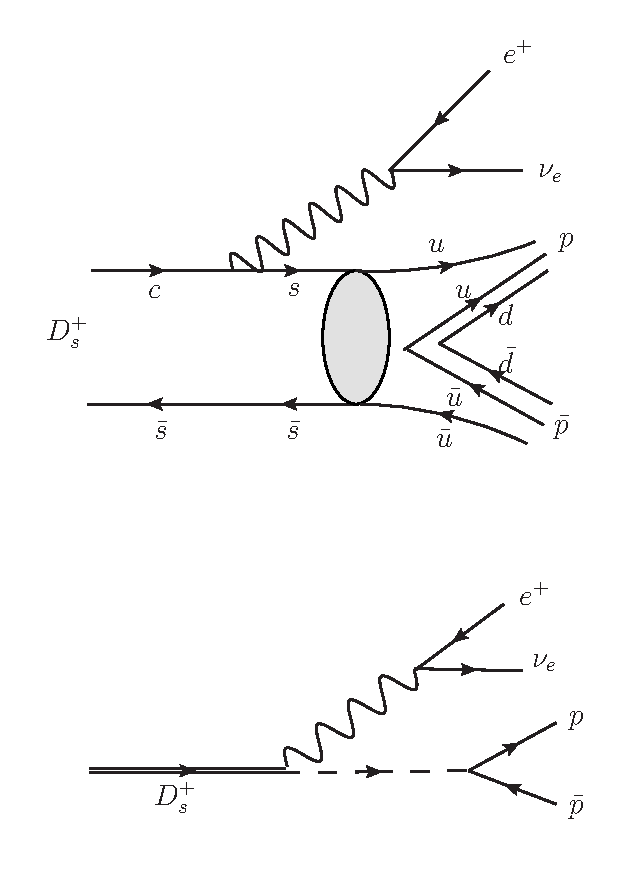
\includegraphics[width=0.8\linewidth]{dsToPPbar/intr/meson-exchange.eps}
    \caption{由介子交换引起的衰变$D_{s}^{+} \to p \bar{p} e^{+} \nu_{e}$
    示意图。}%
    \label{fig:meson-exchange}
\end{figure}
本文将从数据样本、测量方法、
信号重建、测量结果、系统误差分析出发介绍对
$D_{s}^{+} \to p \bar{p} e^{+} \nu_{e}$的寻找。

\section{测量方法}\label{sec:method}
由于相空间的限制,末态粒子的能量都较低,其中电子的能量最低,大约90MeV/c,很难被
探测器重建出来。另外中微子不能被探测器重建。面对重重困难,我们另辟蹊径,
决定在双标记方法的基础上采取
部分重建算法。首先我们选择若干个分支比大、本底低的衰变道重建一个$D_{s}^{-}$
介子,这样的衰变道称之为单标记道,被重建出的介子称为单标记$D_{s}^{-}$。单标记
道的选取原则和具体的挑选过程将在后文中详细介绍。接着我们在剩余的径迹里挑选选
出所关心的信号。由于质子和其他带电粒子的之间的误鉴别率很低,一对相交的电荷相反
的径迹被鉴别为质子对可以作为信号存在的强有力证据,我们仍旧把单标记$D_{s}^{-}$
的不变质量作为观测里来获取信号的产额。

\subsection{分支比的计算公式}

\section{样本}\label{sec:sample}
\subsection{数据样本}
数据样本选用2016年在能量点4.178GeV采集的数据,积分亮度为3.19fb,其中的opencharm末态
$D^{+}D_{s}^{*-}$是用了寻找$D_{s}^{+}$介子的衰变过程。

\subsection{模拟样本}
\subsubsection*{Generic MC}
BESIII产生的蒙特卡洛样本重要用来做本底估计,主要的成份在表~\ref{tab:generic
mc}列出
\begin{table}[htpb]
    \centering
    \caption{Generic 蒙特卡洛样本的主要构成}%
    \label{tab:generic-mc}
    \begin{tabular}{l  c  c  c}
        \toprule 
        物理过程 & 截面  &产生子 & 模拟亮度/数据亮度 \\
        \midrule 
        $D^{0} \bar{D}^{0}$             & 0.179 & BesEvtGen + conExc & 40 x \\
        $D^{+} D^{-}$                   & 0.197 & BesEvtGen + conExc & 40 x \\
        $D^{0} \bar{D}^{*0} + c.c$      & 1.211 & BesEvtGen + conExc & 40 x \\
        $D^{+} \bar{D}^{*-} + c.c$      & 1.296 & BesEvtGen + conExc & 40 x \\
        $D^{*0} \bar{D}^{*0} $          & 2.173 & BesEvtGen + conExc & 40 x \\
        $D_{s}^{+} D_{s}^{-} $          & 0.007 & BesEvtGen + conExc & 40 x \\
        $D \bar{D}^{*}\pi^{\pm} + c.c $ & 0.383 & BesEvtGen + conExc & 40 x \\
        $D \bar{D}^{*}\pi^{0} + c.c $   & 0.192 & BesEvtGen + conExc & 40 x \\
        $D \bar{D}\pi^{\pm} + c.c $     & 0.050 & BesEvtGen + conExc & 40 x \\
        $D \bar{D}\pi^{0} + c.c $       & 0.025 & BesEvtGen + conExc & 40 x \\
        \midrule 
        $e^{+} e^{-} \to q\bar{q}(u, d, s)$ & 13.8 & KKMC & 40 x \\
        \midrule 
        $e^{+}e^{-} \to \gamma_{ISR} J/\psi$     & 0.40 & KKMC & 40 x \\
        $e^{+}e^{-} \to \gamma_{ISR} \psi(3686)$ & 0.42 & KKMC & 40 x \\
        $e^{+}e^{-} \to \gamma_{ISR} \psi(3770)$ & 0.06 & KKMC & 40 x \\
        \midrule 
        $e^{+}e^{-} \to e^{+} e^{-} $       & 423.99 & Babayaga & 0.4 x \\
        $e^{+}e^{-} \to \mu^{+} \mu^{-} $   & 5.24   & Babayaga & 40 x \\
        $e^{+}e^{-} \to \tau^{+} \tau^{-} $ & 3.45   & KKMC & 40 x \\
        \midrule
        two-photon fusion & 1.7 & BesTwogam & 40 x \\
        $\pi \pi (\psi(2S)/h_{c}/J/\psi), (KK/\eta)J/\psi$ & 0.1 & BesEvtGen +
        conExc & 40 x \\
        \bottomrule
    \end{tabular}
\end{table}
\subsubsection{信号模型}
$p\bar{p}$可能不是由直接衰变而来,而是通过一个共振态间接产生。其一,此时的
$p\bar{p}$刚好能构成$X(1835)$,这时共振态的贡献将远大于非共振态,
很多分波分析都验证了这个结论。其二,
多数的半轻过程显示了非共振态的成分要比共振态低的多。因此,我们假定
$D_{s}^{+} \to X e^{+} \nu_{e}$, $X\to p \bar{p}$,其中$X$为中间共振态,可能是赝标量、矢量粒子或者更高自旋的粒子。

\begin{figure}[htbp]
      \centering
          \begin{overpic}[width=8cm]{dsToPPbar/producFeymann.eps}
              \put(10,20){\small {$D_{s}^{+}$}}
              \put(45,20){\small {$X(p\bar{p})$}}
              %\put(45,20){\small {$\eta _{1760}$}}
              %\put(45,15){\small {$f_{2,1810}$}}
              \put(30,8){$\bar{s}$}
              \put(15,32){$c$}
              \put(47,32){$s$}
              \put(87,43){$\nu_e$}
              \put(87,54){$e^{+}$}
              \put(103,30) {$p$}
              \put(103,4) {$\bar{p}$}
          \end{overpic}    
      \caption{$p\bar{p}$对产生示意图。$D_{s}^{+}$介子释放一个$W$玻色子并产生
      共振态$X(p\bar{p})$,这个共振态瞬间产生$p\bar{p}$对。
      }%
      \label{fig:feynman-diagram}
  \end{figure}
这个过程的转移动量依赖的分宽度形式为
\begin{equation}
    \frac{d \Gamma(D^{+}_{s} \to X e^{+} \nu_{e})}{d q^{2}}
    = \frac{G_{F}^{2} |V_{cs}|^{2}}{24 \pi^{3}} p_{X}^{3} |f_{+}(q^{2})|^{2}
\end{equation}
其中$G_{F}$为费米常数,$|V_{cs}|$为CKM矩阵元,$p_{X}$为共振态在$D_{s}^{+}$质心系下的动量大小,$q$是转移动量为$D_{s}^{+}$
和$X$的动量的差, $f_{+}(q^{2})$是形状因子。我们采用ISGW2模型来描述$f_{+}(q^{2})$,其形式为
\begin{equation}
    \label{eq:f_q2}
    f_{+}(q^2) = f_+(q^{2}_{\rm \max}) \left( 1 + r^{2} /12 (q^{2}_{\rm max} - q^{2}) \right)^{-1},
\end{equation}
其$r$是的有效半径,$q_{\rm \max}^{2}$是$q^{2}$的在$D_{s}^{+}$衰变运动学
约束下最大值。
我们用这个模型来产生信号蒙特卡洛样本模拟样本以进行进一步的研究工作。
为了讨论模型不确定带来的影响,我们分别采用了不同宽度、不同质量、不同自旋的X假设,并
产生了不同的样本为后续的研究提供方便。

\section{信号重建}%
\label{sec:reconstruction}
\subsection{带电粒子的重建}%
\label{sec:charged-track}
信号的重建从径迹开始。首先,我们要挑选好的带电径迹,既能通过卡曼滤波条件,并且在探测器的接受范围内。具体的要求如下:
\begin{itemize}
    \item 
带电径迹的初始动量方向的极角满足:$|\cos \theta | < 0.93$;
    \item 
$x$-$y$平面内带电径迹与$e^{+}e^{-}$对撞顶点的投影距离满足:$R_{xy} < 1 cm$; (来自$K_{s}^{0}$的带电径迹除外)
    \item 
$z$方向上带电径迹与$e^{+}e^{-}$对撞顶点的投影距离满足:$R_{z} < 10 cm$。(来自$K_{s}^{0}$的带电径迹除外)
\end{itemize}
其中$e^{+}e^{-}$的的顶点信息从BESIII的对撞顶点数据库中读取。
为了从这些带电径迹中挑选出质子、电子、$\pi$介子、和$K$介子样本,我们采用BESIII上通用的粒子鉴别程序(particleID)来进行
粒子鉴别。该粒子鉴别程序结合电离能损信息(dE/dx)与时间飞行信息(TOF)给出每一条带电径迹为某种粒子(质子、电子、
$\pi$介子、$K$介子)的置信度$P$。
我们要求质子(电子、$\pi$介子、和$K$介子)候选者满足
$P(p) > P(\pi)$, $P(p) > P(K)$。
\subsection{$K_{s}^{0}$介子的重建}
由于$K_{s}^{0}$介子飞行较长的时间,会在对撞顶点之外衰变到$\pi^{+} \pi^{-}$对。为了重建$K_{s}^{0}$介子,我们首先要找
到一对径迹相交电荷相反的带电粒子,它们必须满足
\begin{itemize}
    \item 
带电径迹的初始动量方向的极角满足:$|\cos \theta | < 0.93$;
    \item 
$z$方向上带电径迹与$e^{+}e^{-}$对撞顶点的投影距离满足:$R_{z} < 20 cm$。
\end{itemize}

接着对找到了这对粒子做顶点拟合,要求
$\chi^{2} < 100$;
$ l / \sigma_{l} > 2$。
由于的衰变顶点不同于对撞点,我们可以较好的把衰变来的和其他带电粒子区分开来,因此不在做粒子鉴别。
\begin{figure}[htpb]
    \centering
    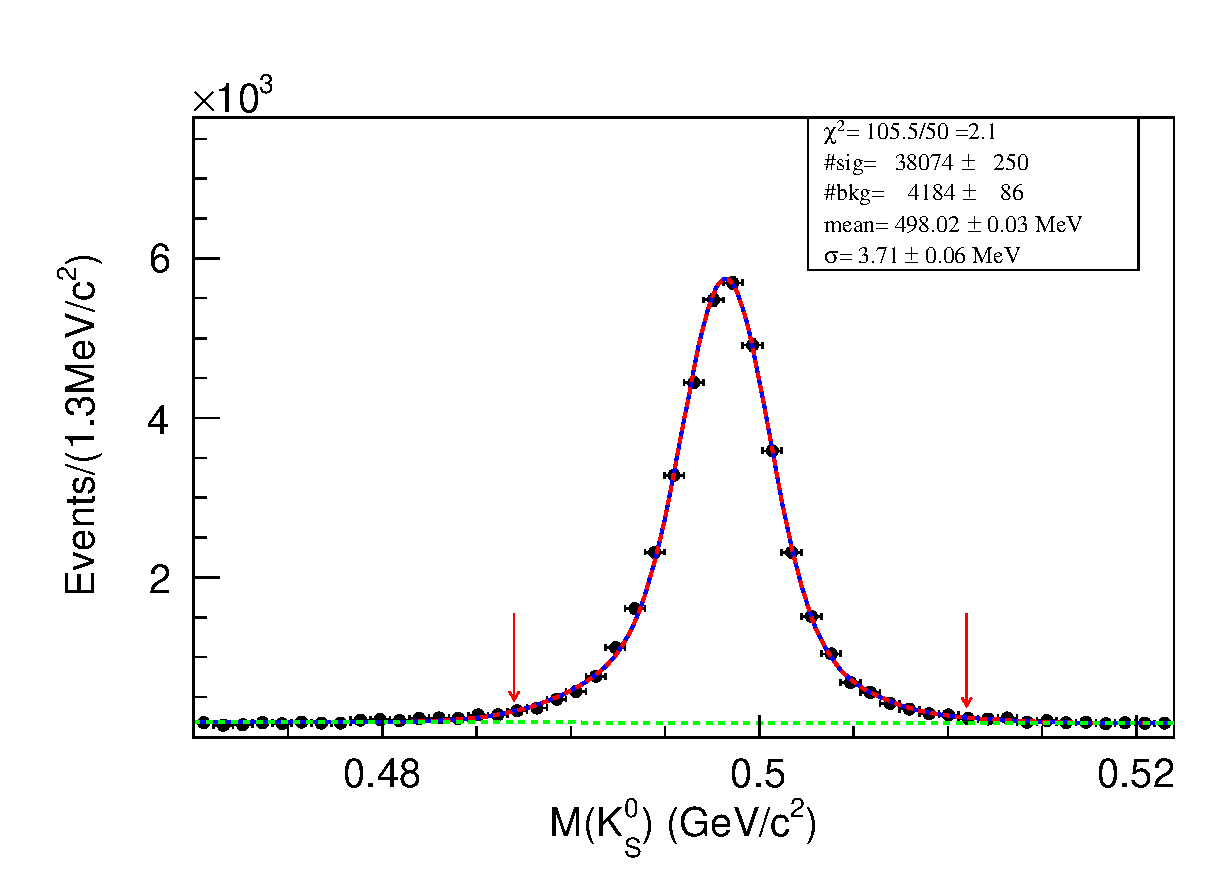
\includegraphics[width=0.8\linewidth]{dsToPPbar/mks.eps}
    \caption{$K_{S}^{0}$的不变质量谱}\label{fig:mks}
\end{figure}
\subsection{中性径迹的重建}
\label{sec:ds-neutral-track}
中性径迹指量能器所重建的电磁簇射,包含发生电磁簇射的位置及沉积能量的信息。实验上,光子会在量能器上沉积大部分能量、带电轻强子、
$K_{L}$和中子都
有一定的几率沉积少量的能量。我们主要的目标是重建光子。
对于用来重建 $\gamma$ 的中性径迹,我们有如下要求:
\begin{itemize}
    \item 在~EMC~桶部区域~($|\cos\theta| < 0.8$)~的沉积能量满足:$E > 25$ MeV;
\item 在~EMC~端盖区域~($0.86 < |\cos\theta| < 0.92$)~的沉积能量满足:
    $E > 50$MeV;
\item 径迹到达~EMC~的飞行时间满足:$0 \leqslant T \leqslant 14\,(\times 50 \,
    {\rm ns})$;
\item 与任何带电径迹在~EMC~上的沉积位置的距离大于~10~倍的标准偏差
    以排除带电径迹的带来的能量沉积。
\end{itemize}

\section{单标记分析}
按双标记方法的原则,我们首先重建一个$D_{s}^{-}$介子以做标记。我们选择单标记信号道的原则是产额大、本底低。我们经过比较选出了
三个最佳的标记道,它们是$K_{S}^{0} K^{-}$,$K^{+} K^{-} \pi^{-}$, 
$K_{S}^{0} K^{+} \pi^{-} \pi^{-}$。
\subsection{候选$D_{s}^{-}$}
以$K_{S}^{0}K^{-}$标记道为例来说明如何重建标记$D_{s}^{-}$介子。
首先按Sec.~\ref{sec:reconstruction}中叙述的方法
分别挑选出$K_{S}^{0}$和$K^{-}$所有的候选者。二者的所有组合都可能是
我们要寻找的$D_{s}^{-}$产物,我们用它们来推断$D_{s}^{-}$
运动学信息。每个事例我们只保留一个最佳的组合,也就是候选$D_{s}^{-}$,选取的原则的$M_{rec}(K_{S}^{0}K^{-})$最接近$m_{D^{*}_{s}}$,
其中$m_{D^{*}_{s}}$为$D^{*}_{s}$介子的不变质量,
\begin{equation}
    M_{rec}(K_{S}^{0}K^{-}) = \sqrt{{\left( \sqrt{s} 
       - E_{K_{S}^{0}} - E_{K^{-}} \right)}^{2}  - 
    {\left(\vec{p}_{K_{S}^{0}} + \vec{p}_{K^{-}} \right)}^{2}}.
\end{equation}
这个候选$D_{s}^{-}$被保留以做进一步分析。如果在单个事例中发现多个标记道
的候选,我们将全部保留并逐个处理。

\subsection{多重候选}
在单个事例中,对每个单标记道,我们只保留一个候选$D_{s}^{-}$粒子。为了能够有效
的挑选出正确的组合,我们选择$\Dsm$的反冲不变质量 ($M_{rec}(\Dsm)$)作为重要的
观测量。借鉴CELOc的经验~\cite{Alexander:2008aa},为了提高$M_{rec}(\Dsm)$的
分辨率,我们用如下公式计算$\Dsm$的能量
\begin{equation}
    E_{\Dsm} = \sqrt{m_{\Dsm}^{2} + |\vec{p_{\Dsm}}|^{2}},
\end{equation}
式中$m_{\Dsm}$为$\Dsm$的静止质量。相应的$M_{rec}(\Dsm)$可以写为
\begin{equation}
    M_{rec} \left( \Dsm \right)  =  \sqrt{%
        \left( E_{cm} - E_{\Dsm} \right){}^{2}
    - p_{\Dsm}^{2}  },
    \label{def:mrec}
\end{equation}
反冲不变质量$m_{rec}(\Dsm)$的分布如图~\ref{fig:recmassMC}所示,从$D^{*-}_{s}$
衰变出来的$\Dsm$介子的反冲不变质量为一个平台,但是从$e^{+}e^{-}$直接产生
$\Dsm$介子则会形成一个明显的峰结构,峰值恰好在$D_{s}^{*+}$的不变质量处。综合
考虑,我们选择$M_{rec}(\Dsm)$最接近$m_{D_{s}^{*+}}$的候选组合作为唯一的
$D_{s}^{-}$候选。

\subsection{单标记道的本底分析}
本底的主要来源包括:open charm和连续性本底。前者的$M_{rec}$不变质量远离信号
区,如图~\ref{fig:recmassMC}所示。为了压制这样的本底我们要求$D_{s}^{-}$的反
冲不变质量$M_{rec}$满足下列条件:
\begin{itemize} 
    \item $2.06 < M_{rec}(\Dsm) < 2.18 $ GeV $/c^{2}$ 
\end{itemize}

\begin{figure}[htbp]
    \centering
    \mbox{%
        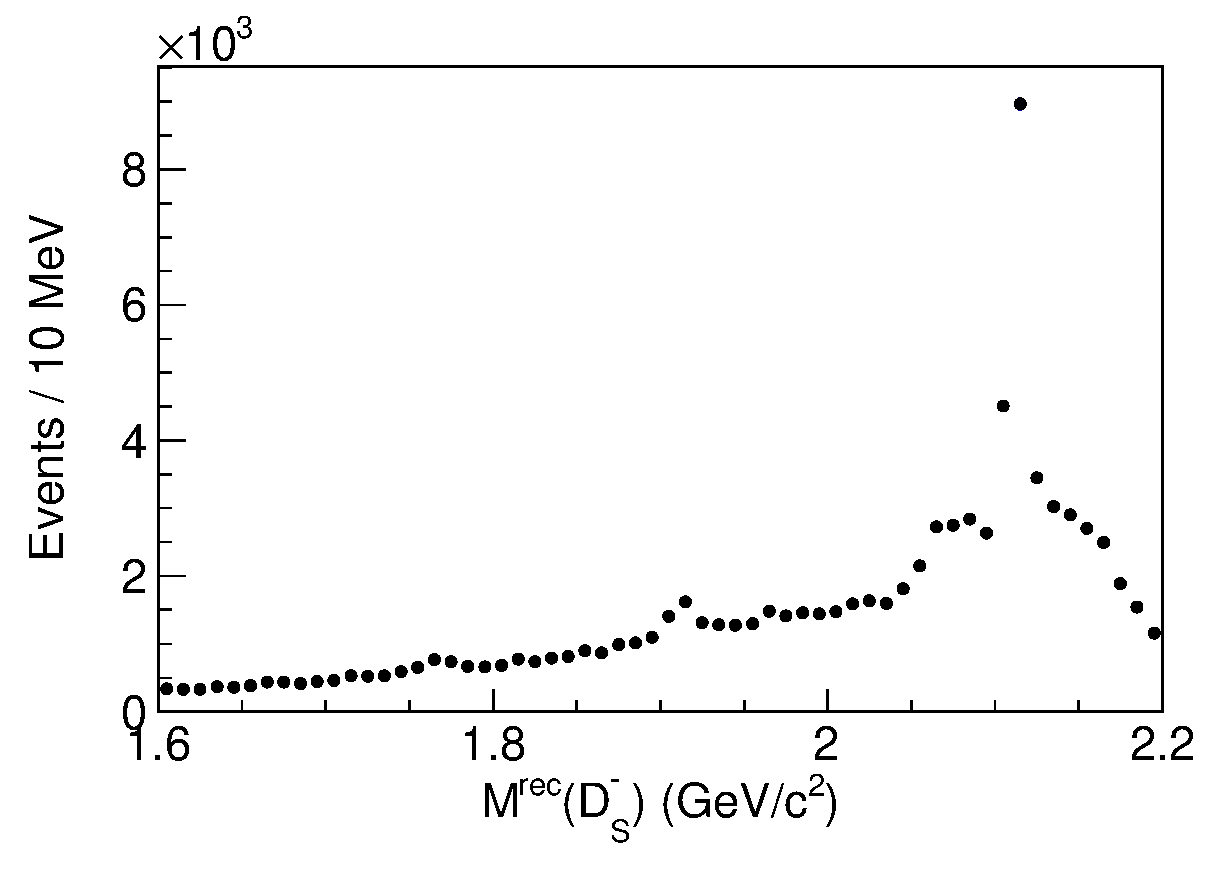
\includegraphics[width=0.8\linewidth]{dsToPPbar/recmass.eps}
    }
    \caption{标记$D_{s}^{-}$介子的反冲不变质量谱。
    }%
    \label{fig:recmassMC}
\end{figure}
此外,我们发现有一种主要的峰本底来自衰变$D^{*} \to D \pi$,由于从$D^{*}$衰变
出来的$\pi$介子动量很低,如图~\ref{Fig:pion_momentum}所示。
为了压低这个峰本底,我们要求$\pi$的动量大于100 MeV。
\begin{figure}[htbp]
    \centering
    \mbox{%
        \begin{overpic}[width=0.6\linewidth]{dsToPPbar/ppion.eps}
            %\put(50,70) {\color {green} {$ K^{+} K^{-} \pi ^{-} $}}
        \end{overpic}
    } 
    \caption{$\pi$介子的动量分布图。黑色的带误差棒的点代表数据,蓝色和红色
    的实线分别展示了$D_{s}^{*+}D_{s}^{-}$和$D^{*}D$蒙特卡洛样本中的动量分布。
    我们能发现一个明显由$D^{*}$衰变引起的峰结构。
    }\label{Fig:pion_momentum}
 \end{figure}
\subsubsection{峰本底}
在三个单标记道道中,只有$K_{S}^{0}K^{-}$由一种峰本底无法压制,这个峰本底
来自$D^{-}\to K_{S}^{0} \pi^{-}$,其中的$\pi^{-}$被误鉴别为$K^{-}$,不变质量
谱向右移动,从而形成峰本底。

\subsection{单标记产额和效率}

\subsubsection{拟合方法}
这些候选$D_{s}^{-}$既可能是我们需要的信号,也有可能为错误的组合(本底)。
信号事例和本底事例的不变质量谱形截然不同,
因此为了获得标记道的信号产额,我们把$D_{s}^{-}$的不变质量作为观察量。
我们决定采取极大似然法拟合$D_{s}^{-}$的不变质量分布来
获得信号产额。似然量的定义为
\begin{equation}
    L = e^{-N} \frac{N^{n}}{n!} 
    \prod_{i=1}^{i=N} \left( 
    \frac{n_{sig}}{n}  P_{sig}(m_{i}) 
    +  \frac{n_{bkg}}{n} P_{bkg}(m_{i})
\right),
\end{equation}
式中$N$,$n$ 分别为预期的总事例数和观测值, 
$n$为样本的中候选$D_{s}^{-}$个数,
$m_{i}$为第$i$个候选$D_{s}^{-}$的不变质量,
$P_{sig}$和$P_{bkg}$分别是信号和本底的概率
密度函数,
$n_{sig}$和$n_{bkg}$是同概率密度的参数分别指信号数和本底数。
拟合的过程也就是求似然函数极大值的过程,此时$n_{sig}$即为信号的产额。

\subsubsection{拟合模型的构造}
\begin{figure}[htbp]
    \mbox{%
        \begin{overpic} [width=0.45\linewidth] {dsToPPbar/Ds_mc401.eps}
            \put(80, 55){\color{blue} {(1)} }
        \end{overpic}

        \begin{overpic} [width=0.45\linewidth] {dsToPPbar/Ds_mc400.eps} 
            \put(80, 55){\color{blue} {(2)} }
        \end{overpic}

    }
        \begin{overpic} [width=0.45\linewidth]{dsToPPbar/Ds_mc406.eps} 
            \put(80, 55){\color{blue} {(3)} }
        \end{overpic}

    \caption{标记侧的$M(D_{s}^{-})$分布及拟合结果。
        数据是带误差棒的黑色点。标记道分别是 (1)
        $K^{+}K^{-}\pi^{-}$ (2) $ K_{S}^{0} K^{-}$ 
        (3)$ K_{S}^{0} K^{+}\pi^{-}\pi^{-}$.
    }\label{Background_analysis_for_ST_modes}
\end{figure}
图\ref{Background_analysis_for_ST_modes}是数据和蒙特卡洛样本之间的对比,从图中我们
可以看出蒙特卡洛模拟的足够好,除了单标记道$K_{S}^{0}K^{-}$以外,均没有明显的峰状
本底。因此我们用切比雪夫多项式描述本底的形状。我们尝试用双高斯分部描述MC
中信号的形状,为了补偿数据和蒙特卡洛样本之间的分辨率差异,我们把经高斯函数卷积后的
信号蒙特卡洛样本的形状描述数据中的信号形状,其中的高斯函数的中心值和分辨作为自由参数
由数据决定。
\subsection{拟合结果}
\begin{figure}[htpb]
    \centering
    \mbox{%
        \begin{overpic}[width=0.45\linewidth]{dsToPPbar/Ds401.eps}
            \put(30, 50){\color{blue} {(1)}}
        \end{overpic}
        \begin{overpic}[width=0.45\linewidth]{dsToPPbar/Ds400.eps}
            \put(30, 50){\color{blue} {(2)}}
        \end{overpic} 
    }
        \begin{overpic}[width=0.45\linewidth]{dsToPPbar/Ds406.eps}
            \put(30 ,50) {\color{blue} {(3)} }
        \end{overpic}
    \caption{%
        不同标记道中的$D_{s}^{-}$不变质量谱的拟合结果。
        三个标记道分别是 (1) $K^{+}K^{-}\pi^{-}$ 
        (2) $K_{s}K^{-}$ (3) $K_{S} K^{+}\pi^{-}\pi^{-}$。 
        红色的点虚线是峰本底的贡献。
    }%
    \label{fig:ST_data_fit}
\end{figure}
效率的定义为
\begin{equation}%
    \label{eq:ST-efficiency}
    \epsilon = \frac{N^{ST}}{N^{generated}}
\end{equation}
式中$N^{ST}$是标记$D_{s}^{-}$的产额,$N^{generated}$则是样本中
该标记$D_{s}^{-}$ 总数目。拟合的结果如图\ref{fig:ST_data_fit},相关
的效率在表\ref{table:ST_yield_and_efficiency}做了汇总。
\begin{table}[htbp]
    \centering
    \begin{tabular}{l l c c c c}
        \toprule[0.2em]
        标记道 ($\alpha$) & 次级衰变 & 产额 (MC) & 总数 & $\epsilon^{ST}(\%)$ &
        产额 (data)
        \\     
        \midrule
        $D_{s}^{-}\rightarrow K^{+}K^{-}\pi^{-} $ &-
        & 2642391 $\pm$ 2455 & 6243628 &    42.32    $\pm$    0.04      &  140277$\pm$ 635
        \\  

        $D_{s}^{-}\rightarrow K_{s}K^{-} $ & $K_{S}^{0}\rightarrow \pi^{+}\pi^{-}$ 
        & 565897 $\pm$ 2025 &     1147161     &    49.33    $\pm$    0.18  & 31267 $\pm$ 261
        \\ 

        $D_{s}^{-}\rightarrow K_{s}K^{+}\pi^{-}\pi^{-} $ & $K_{S}^{0} \rightarrow \pi^{+}\pi^{-} $ 
        & 272531 $\pm$ 925 &    923848    &    21.08    $\pm$    0.07  & 14547
        $\pm$ 214 \\
        \bottomrule
    \end{tabular}
    \caption{单标记效率及数据中各个标记道产额。
    }\label{table:ST_yield_and_efficiency}
\end{table}

\section{信号道的重建}\label{Double-Tag}
\subsection{信号挑选}
信号侧的$D_{s}^{+}$介子衰变到$p\bar{p}e^{+}\nu_{e}$。
如前文讨论,电子由于动量过低而难以被重建,因此重要的信号是发现正反
质子对,能够发现电子作为一个辅助手段。当电子恰好被完整重建时,我们
重建这个电子作为压低本底的一个手段。
基于信号蒙特卡洛样本,本文首先详细研究了电子被重建的几率。图\ref{Fig:tracks}
展示了信号蒙特卡洛样本中标记一个$D_{s}^{-}$之后剩余的带电径迹数目的分布,
我们发现发现三条径迹的情况仅仅占6.8\%,这意味着至少有93\%以上的电子
丢失了。
\begin{figure}[htbp]
    \centering
    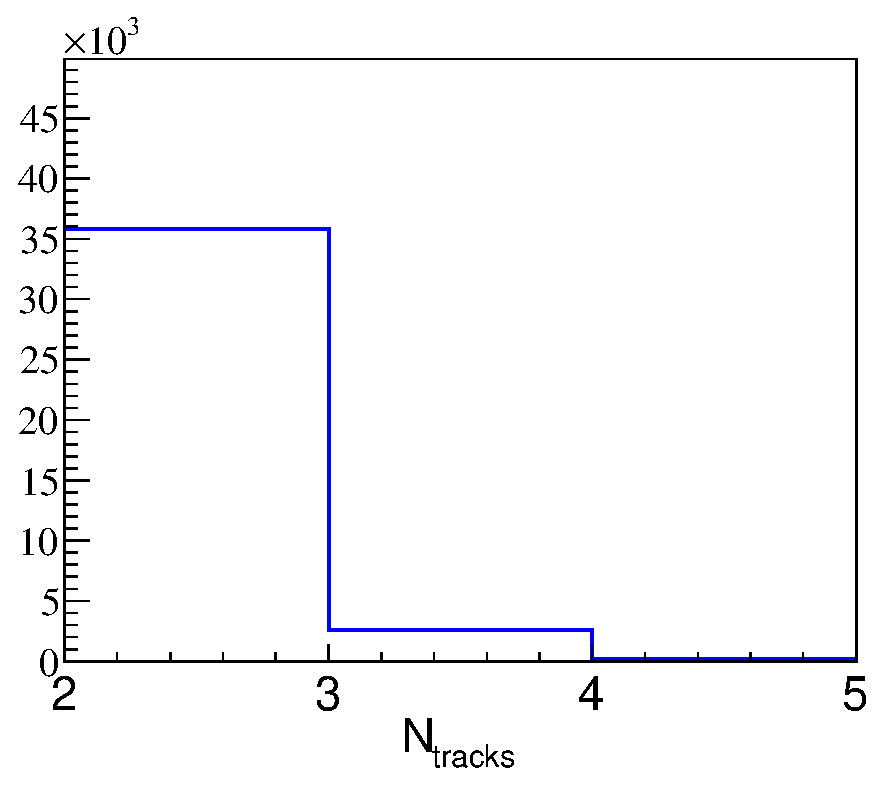
\includegraphics[width = 8 cm]{dsToPPbar/Tracks_signalMC.eps}
    \caption{信号蒙特卡洛样本中的带电径迹数目(除了标记侧)分布。
    }\label{Fig:tracks}
\end{figure}
因此我们按带电径迹个数把样本分为两类:
\begin{itemize}
    \item \textbf{A}: 仅有两条带电径迹,并且被鉴别为正反质子对
    \item \textbf{B}:有三条带电径迹,其中有一对带电径迹被鉴别为正反质子对
\end{itemize}
我们将在下文里对两种情况分别进行讨论。

\subsubsection{进一步讨论}
\subsubsection{质子和电子的动量信息}
在带电粒子中,质子的MDC中的电离能损最大。在BESIII的探测器上,动量低于
200MeV$/c$的质子,其径迹不可能被重建。因此图中\ref{Fig:momenta_of_proton},
质子的动量谱在220MeV$/c$附近急剧下降。但是仍有少数事例存在误鉴别的质子,
造成动量谱在200MeV$/c$以下不为0,故而,为了压低本底,我们要求质子的
动量大于200MeV$/c$。
\begin{figure}[htbp]
    \centering
    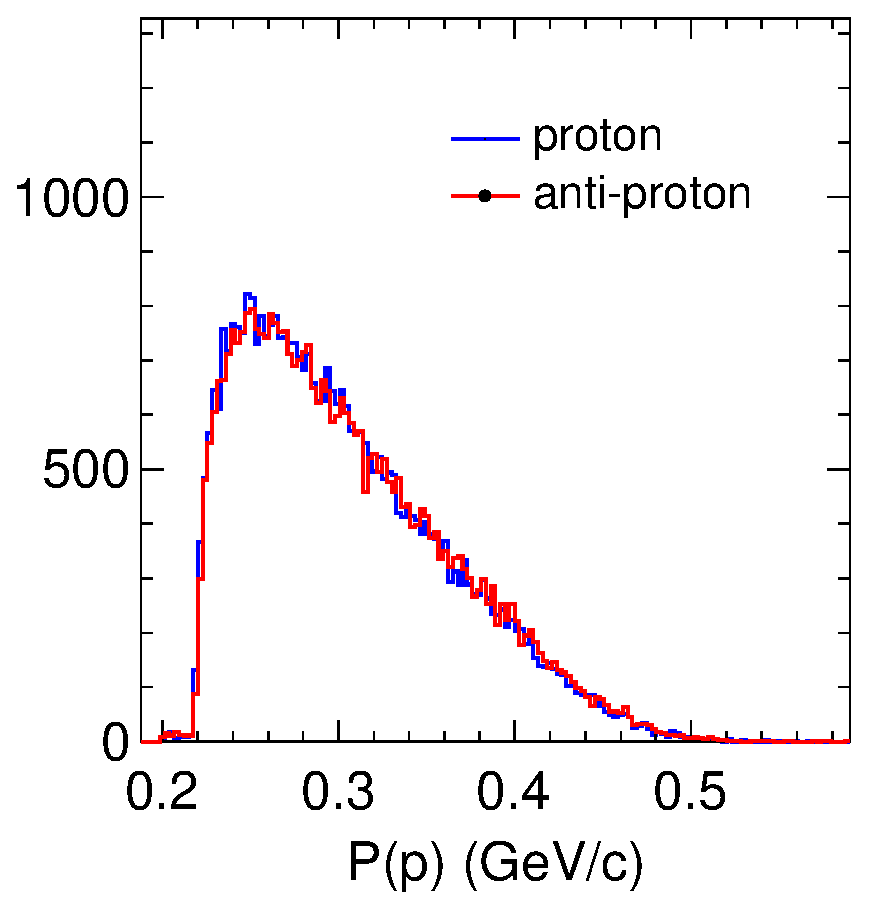
\includegraphics[width = 8 cm]{dsToPPbar/Momentum_proton_signalMC.eps}
    \caption{信号蒙特卡洛样本中正反质子对的动量分布。红色和蓝色的实线分别代表质子和
    反质子。
    }\label{Fig:momenta_of_proton}
\end{figure}
另一方面,由于相空间的限制,电子的动量低于90MeV$/c$,在情况\textbf{B},我们
能清晰地把质子和电子区分开,不必对电子做任何粒子鉴别。如图\ref{Fig:pele}
所示,在遍举蒙特卡洛样本中存在其他粒子被误作为电子,本文根据它们之间的动量分布
的不同,对电子的动量做要求能显著的压低这种本底。

类似的,本文定义了\textbf{FOM}来优化电子的选择条件,\textbf{FOM}的定义为
\begin{equation}
    FOM = \frac{S}{\sqrt{B}}, 
    \label{eq:FOM-ele}
\end{equation}
式中$S$和$B$分别是信号数和本底个数,其中$S$从信号
蒙特卡洛样本中得到,$B$则在混合蒙特卡洛样本中取得。

从\textbf{FOM}~\ref{Fig:pele}的曲线可以看出,
\textbf{FOM}的值大致在90MeV
达到峰值,这几乎也是电子动量大小的运动学
极限 (\ref{Equ:cut_on_momentum_of_electron}),综合考虑,我们要求 
重建出的电子动量不得大于90MeV. 
\begin{figure}[htbp]
    \centering
    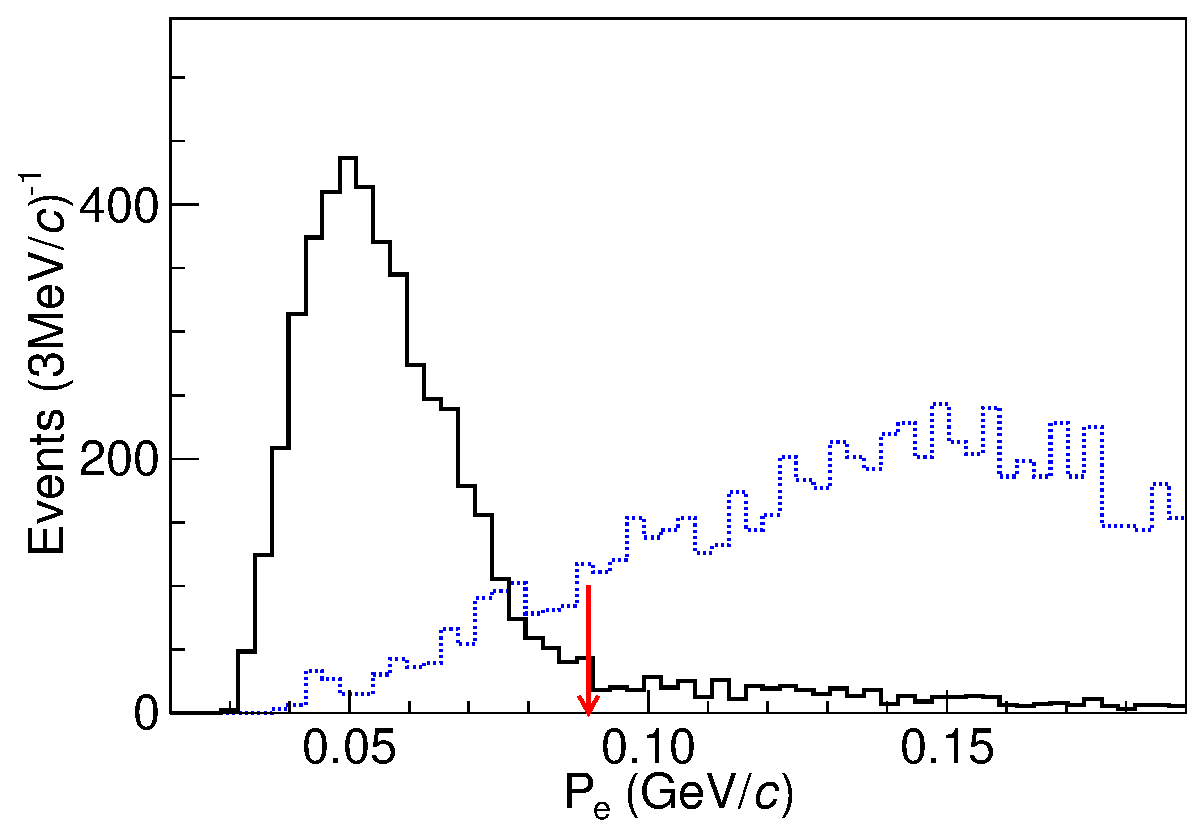
\includegraphics[width = 0.45\linewidth]{dsToPPbar/pele.eps}
    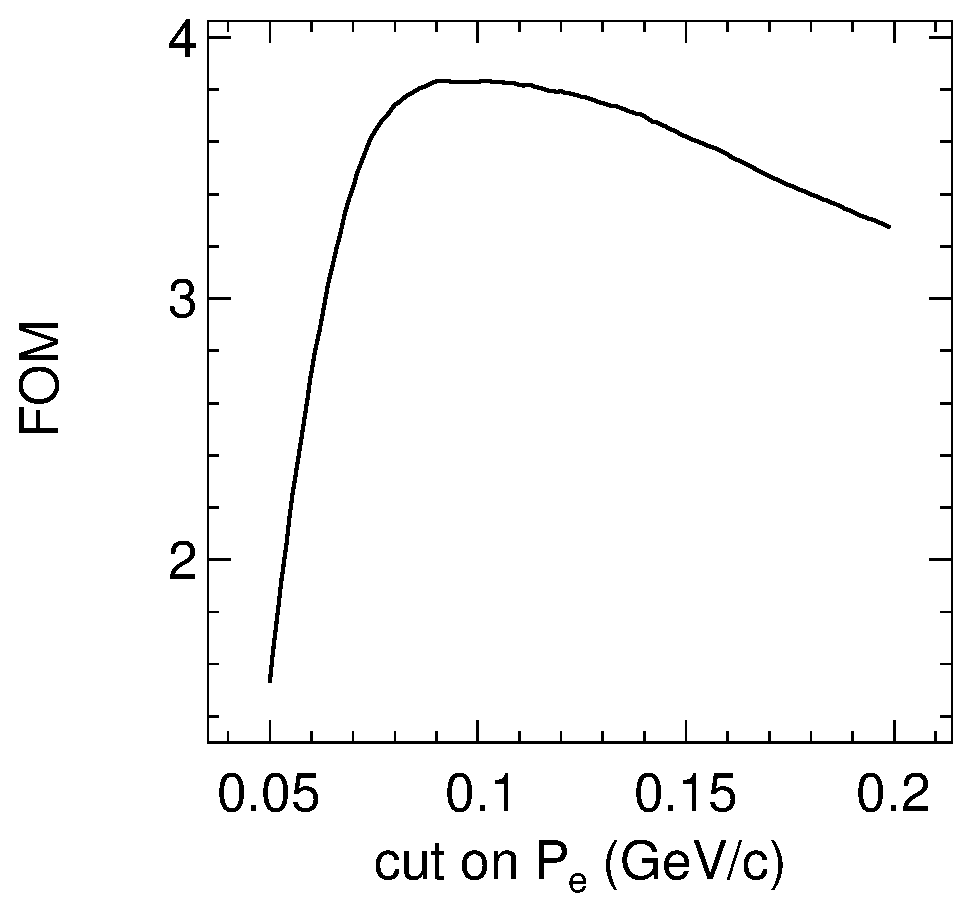
\includegraphics[width = 0.45\linewidth]{dsToPPbar/Optimiz_cut_Pele.eps}
    \caption{左图:电子的动量分部。绿色的实线表示信号形状,
    而蓝色的虚线表示本底的形状。右图: \textbf{FOM}曲线。
    }%
    \label{Fig:pele}
\end{figure}

\subsubsection{$MM^{2}$}
由于半轻道中中微子不能被BESIII探测器重建,因此丢失不变质量常常作为
重要的观测量以此得到中微子的产额。然而在本分析中,除了中微子,90\%
以上的电子也由于难以被探测而丢失,使得丢在不变质量不再是理想的观测量。
然而质子对的存在恰能够推测出电子的存在,根据轻子数守恒,必然存在一个电子
型中微子。这就是本文之所以仅仅把丢失不变质量作为压低本底的手段,而不是
决定信号产额的观测量。本文分两种情况,即是否找到了电子径迹,分别定义了
丢失不变质量,具体的定义见式.~\ref{eq:MM_define}
\begin{equation}
    \begin{aligned}
        \label{eq:MM_define}
        \textbf{2 tracks}: 
        MM^{2} &= {\left( E_{cm} -  E_{ST} - E_{p} - E_{\bar{p}} \right)}^{2} 
        -{\left( p_{p} + p_{\bar{p}} \right) }^{2} 
        \notag \\
        \textbf{2 tracks}:
        MM^{2} &= {\left( E_{cm} -  E_{ST} -E_{p} -E_{\bar{p}} - E_{e}
        \right)} ^{2} - {\left(p_{p} + p_{\bar{p}}  + p_{e} \right)}^{2}
    \end{aligned}
\end{equation}
式中$E_{ST}$ 和 $p_{ST}$ 分别是$e^{+}e^{-}$质心系下标记$\Dsm$的总能量和
总动量,$E_{p}$, $E_{\bar{p}}$,$p_{p}$,和 $p_{\bar{p}}$ 
分别是正反质子相应的能量和动量,$E_{e}$ and $p_{e}$ 分别是电子的能量和动量,
只有在情况\textbf{B}下,我们才在计算$MM^{2}$时计入电子的能量
和动量信息。
如图所示\ref{fig:MMbkg},对于不同的标记道,$MM^{2}$的本底形状大致相同,
峰值均在0.0 ${(GeV/c^{2})}^{2}$, 位于信号的左侧。
\begin{figure}[htbp]
    \begin{center}
    \mbox{%
        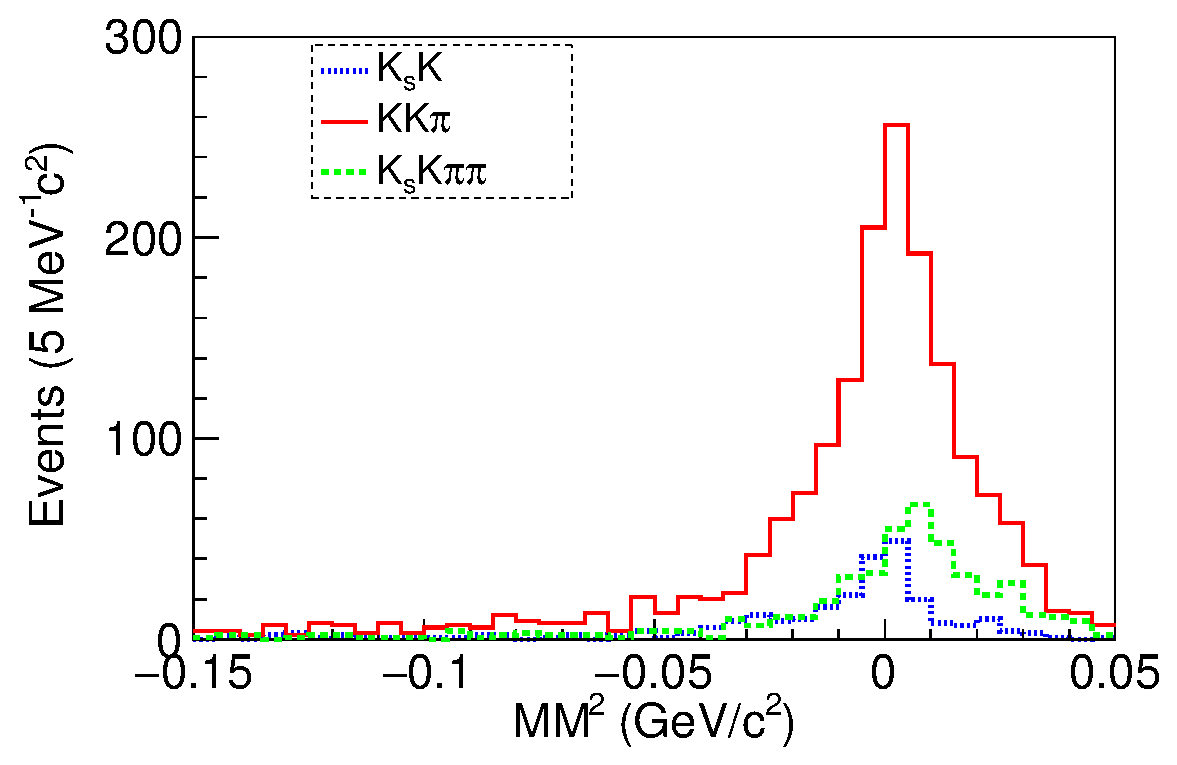
\includegraphics[width = 0.8\linewidth]{dsToPPbar/MMbkg.eps}
    }
    \end{center}
    \caption{$q\bar{q}$样本中$MM^{2}$的分布。红色、蓝色和绿色的实线分别表示
    三个标记道:
    $KK\pi$,$K_{S}^{0}K$ and $K_{S}^{0}K^{-}\pi^{+}\pi^{+}$
    }\label{fig:MMbkg}
\end{figure}

\begin{figure}[htbp]
    \centering
    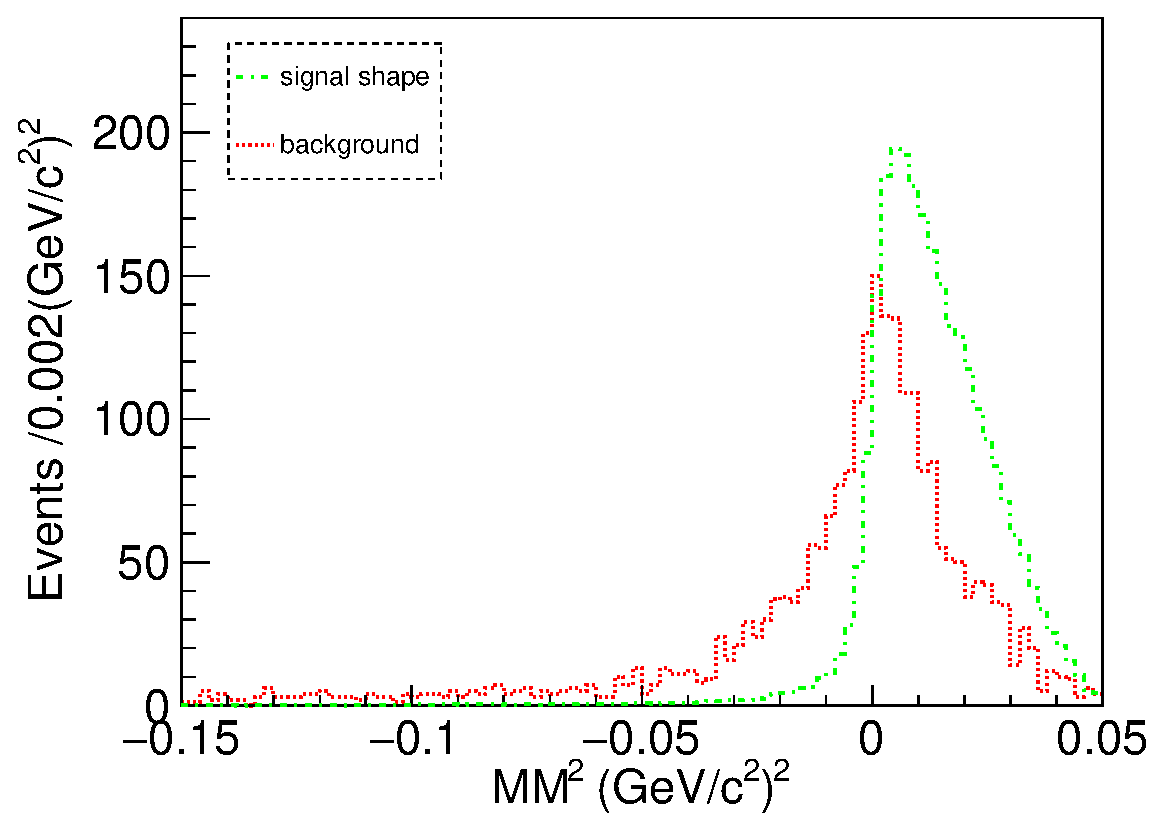
\includegraphics[width = 0.8\linewidth]{dsToPPbar/MC_Sig_compare.eps}
    \caption{合并所有的标记道之后的$MM^{2}$分部。绿色和红色的实线分别
    表示信号和本底的形状。
    }\label{fig:MC_Sig_compare}
\end{figure}
为了研究信号模型对$MM^{2}$的影响,近而确定对$MM^{2}$的要求,我们产生了
两种信号蒙特卡洛样本,得到的$MM^{2}$的形状如图\ref{fig:MM_model}所示。综合考虑
\textbf{FOM}和潜在的系统误差,一方面,如图\ref{fig:FOM}在0.0
${(GeV/c^{2})}^{2}$达到最大值,另一方面,$MM^{2}$ 在大于0.0 
${(GeV/c^{2})}^{2}$区域内形状的不确定性很高,若选择条件右移,会造成
潜在的系统误差。因此本文要求$MM^{2} >0.0{(GeV/c^{2})}^{2}$,后续的研究表明
这个选择条件带来的误差仅仅为1\%。
\begin{figure}[htbp]
    \begin{center}
    \mbox{%
        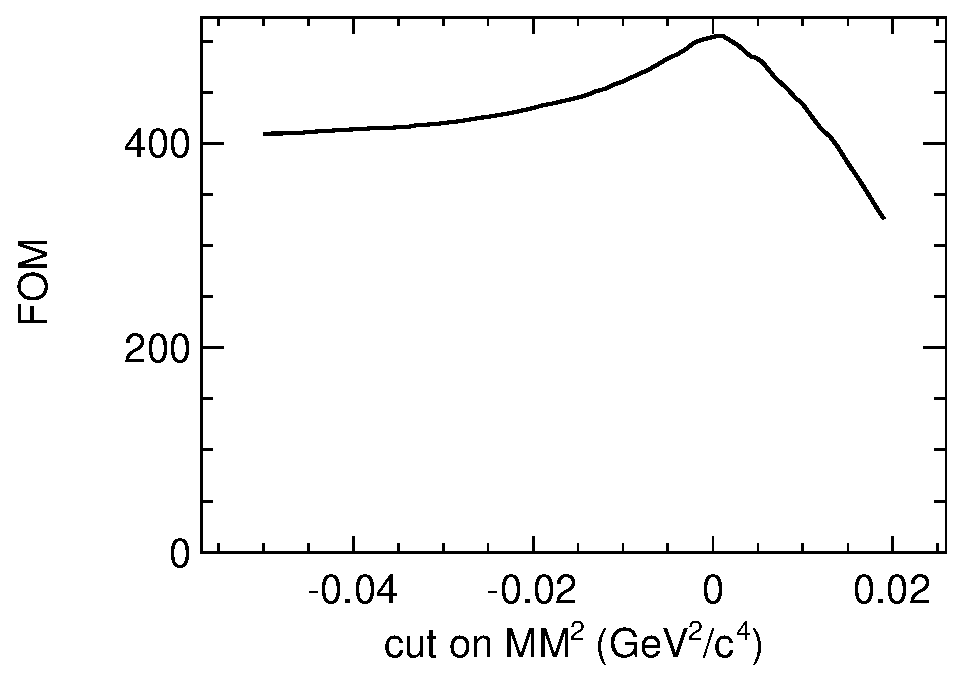
\includegraphics[width = 0.9 \linewidth]{dsToPPbar/Optimiz.eps}
    }
    \end{center}
    \caption{变动对$MM^{2}$的要求。阈值在$0.0 GeV/c^{2}$附近\textbf{FOM}
    达到极大值。
    }\label{fig:FOM}
\end{figure}
\begin{figure}[htbp]% different model
    \centering
    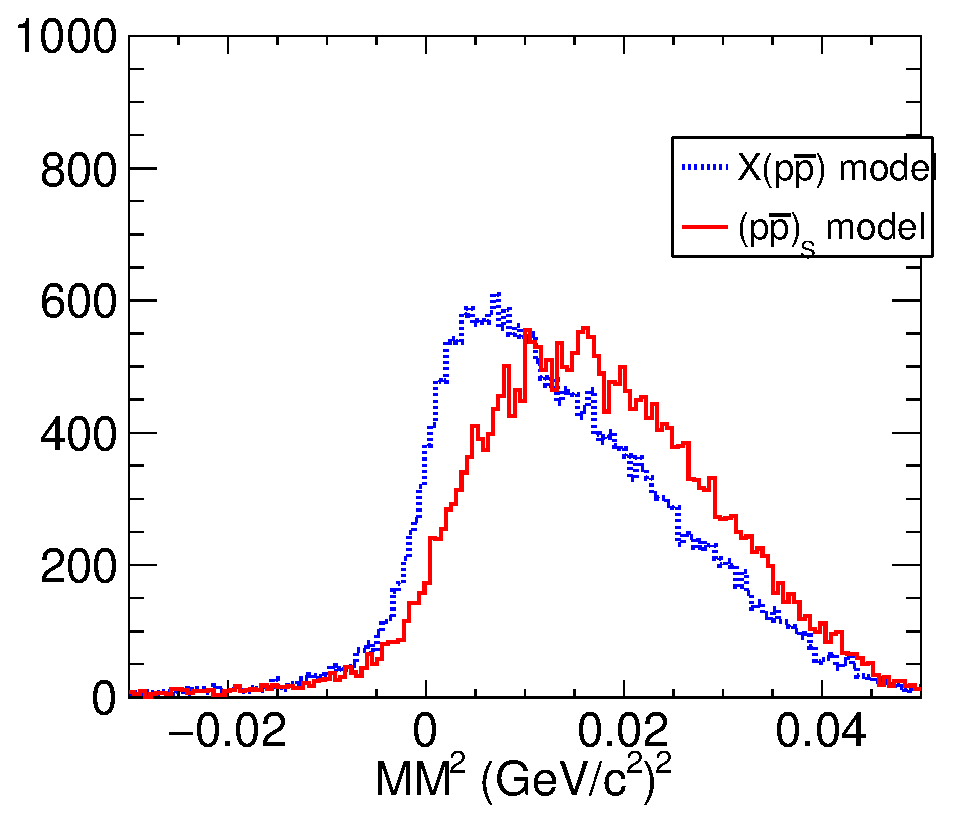
\includegraphics[width=0.9 \linewidth]{dsToPPbar/MMsig.eps}
    \caption{蓝线和红线分别表示模型${(p\bar{p})}_{S}$和$X(p\bar{p})$中
    的信号形状。
    }\label{fig:MM_model}
\end{figure}

\subsubsection{本底分析}
本底的分析过程是基于35倍于数据亮度的混合蒙特卡洛样本。本底的主要来源是$q\bar{q}$
过程,原因是其能产生丰富的正反质子对。从不变质量谱\ref{fig:qq_bkg}上
可以看出没有明显的峰状本底。其他过程中,我们只发现几个open charm过程,
这是由于质子的误鉴别率比较低。对于我们最关心的$D_{s}^{*}D_{s}$过程,
只有3个事例通过了事例挑选程序,从而可以推断出数据中的峰本底要少于0.1个,
这是完全可以忽略不计。
\begin{figure}[htbp]
    \begin{center}
        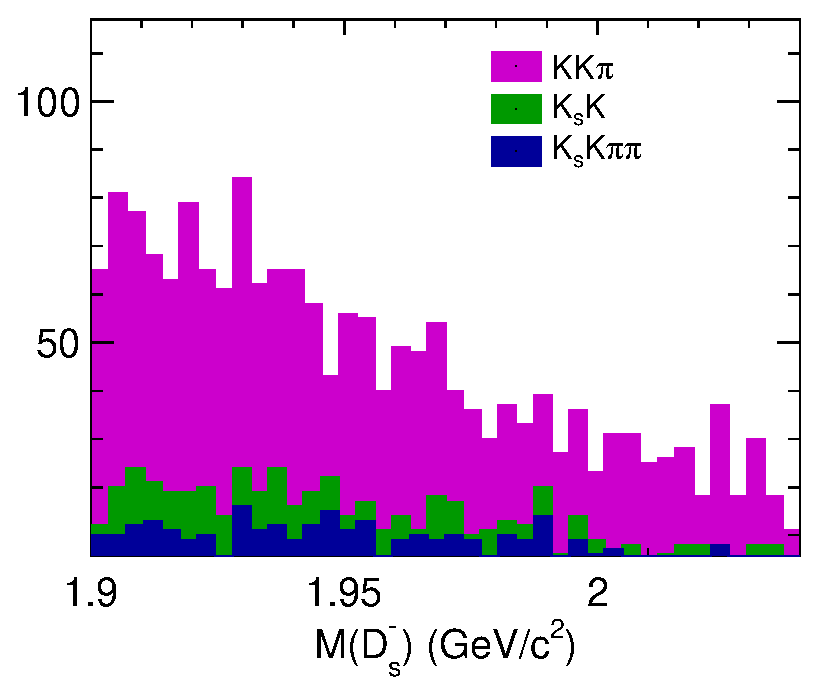
\includegraphics[width=8cm]{dsToPPbar/tag_mass.eps}
    \end{center}
    \caption{$q\bar{q}$样本中的$M(D_{s}^{-})$分布。红色、绿色和蓝色
    的实线分别展示标记道$KK\pi$、$K_{s}K$和
    $K_{s} K^{+} \pi^{-}\pi^{-}$中的不变质量谱。
    }\label{fig:qq_bkg}
\end{figure}
在最大的本底来源--$q\bar{q}$ 中,几种典型的过程为
$e^{+}e^{-} \rightarrow p \bar{p} 4\pi$, 
$p \bar{p} K^{+} K^{-} 2\pi n\pi^{0}$ ($n=0,1,2\cdots$)。前者由于
其中一个$\pi$介子 被误鉴别为$K$介子并和其他的$\pi$介子
误组合成一个$D_{s}^{+}$, 后者则是$K$介子和$\pi$介子直接误组合
成一个$D_{s}^{+}$。
图~\ref{Fig:different_background}则显示这几种典型本底的形状较为相似,
因此我们直接用混合蒙特卡洛样本中的本底形状来描述本底,而把这些典型过程中的本底
形状的细微差异作为一项系统误差来源。

\begin{figure}[htbp]
    \mbox{%
        \begin{overpic}[width = 0.45 \linewidth]{dsToPPbar/Mds_qq_401.eps}
            \put(25,55) {\scalebox{0.7}{$K^{+} K^{-} \pi^{-}$}}
        \end{overpic}

        \begin{overpic}[width = 0.45 \linewidth]{dsToPPbar/Mds_qq_400.eps}
            \put(25,55) {\scalebox{0.7} {$K^{-} K_{s}^{0}$}}
        \end{overpic}
    }
    \mbox{%
        \begin{overpic}[width = 0.45 \linewidth]{dsToPPbar/Mds_qq_406.eps}
            \put(25,55) {\scalebox{0.7}{{$ K_{s}^{0} K^{+} \pi^{-} \pi^{-} $} }}
        \end{overpic}
    }

    \caption{来自几种主要本底信号道中的本底形状。
    }%
    \label{Fig:different_background}
\end{figure}

\subsubsection{双标记效率}%
\label{sec:dt-efficiency}
为了拿到双标记的效率,我们产生了一千万的信号蒙特卡洛样本。在这些样本中,有一个
$\Ds$介子衰变到所有已知的衰变道,另一个$\Ds$介子衰变到信号道。与单标记侧的
分析类似,我们通过拟合标记$\Ds$的不变质量谱来得到信号的产额。
在拟合的过程中,我们借助于工具\textbf{RooKeyPdf}从信号蒙特卡洛样本中直接获取信号形状,
用二阶切比雪夫多项式来描述本底的形状。图\ref{Fig:DT}展示了拟合的结果,
表\ref{table:DT_yield_and_efficiency}中是双标记的产额和效率
\begin{table}[htpb]
    \caption{双标记的产额和效率DT。$\epsilon_{1}$和$\epsilon_{2}$分别表示
    来自模型$X(p\bar{p})$和${(p\bar{p})}_S$的效率。
    }\label{table:DT_yield_and_efficiency}
    \centering 
    \begin{tabular}{lcccc} 
        \toprule
        衰变模式 &  样本大小(事例数)  &  $\epsilon^{ST} (\%)$ & 
        $\epsilon ^{DT}_{1} /\epsilon^{ST}(\%)$  & $\epsilon^{DT}_{2} / \epsilon^{ST} (\%)$
        \\  
        \midrule
        $D_{s}^{-} \rightarrow K^{+} K^{-} \pi^{-}$ & 500000 & $
        42.32 \pm 0.04 $ & $ 16.8 \pm 0.1 $  & $20.4 \pm 0.1$\\
        %16.77
        $D_{s}^{-} \rightarrow K^{-} K_{s}^{0}$ & 500000 &$ 49.33
        \pm 0.18 $ & $ 16.0  \pm 0.1 $ & $19. 5 \pm 0.1$\\

        $D_{s}^{-} \rightarrow K_{s}^{0} K^{+} \pi^{-} \pi^{-} $ &
        500000 &$ 21.08 \pm 0.07 $ & $ 14.8 \pm 0.2$  & $18.1 \pm
        0.2$\\
        \bottomrule
    \end{tabular}
\end{table}

\begin{figure}[htbp]
    \mbox{%
        \begin{overpic}[width = 0.32 \linewidth]{dsToPPbar/Ds401_x1835.eps}
            \put(20,75) {\scalebox{0.7}{$K^{+} K^{-} \pi^{-}$}}
        \end{overpic}

        \begin{overpic}[width = 0.32 \linewidth]{dsToPPbar/Ds400_x1835.eps}
            \put(20,75) {\scalebox{0.7} {$K^{-} K_{s}^{0}$}}
        \end{overpic}

        \begin{overpic}[width = 0.32 \linewidth]{dsToPPbar/Ds406_x1835.eps}
            \put(20,75) {\scalebox{0.7}{{$ K_{s}^{0} K^{+} \pi^{-} \pi^{-} $} }}
        \end{overpic}
    }
    \caption{对信号蒙特卡洛样本中$D_{s}^{-}$不变质量谱的拟合结果。
    黑色的带误差棒的点代表数据,
    蓝色、绿色和红色的线分别表示拟合结果、信号形状和本底形状。
    }\label{Fig:DT}
\end{figure}

\subsubsection{效率修正}%
\label{Sec:Correction_of_Efficiency}
由于低动量的质子和物质(这里指探测器)的相互作用比较复杂,蒙特卡洛模拟和真实
的相互作用有些差异,因此本文利用控制样本首先得到数据和蒙特卡洛样本之间的效率差异,
并进一步修正了双标记的效率。
由于粲介子几乎不衰变到质子,因此本文从$q\bar{q}$过程中选择控制样本,最为
合适的一个样本是 
$e^{+} e^{-} \rightarrow p \bar{p} \pi^{+}\pi^{-}$,具有本底低、样本大的优点。
本文利用这个控制样本做了质子鉴别的系统研究,相关的细节见附录。

本文用观测量$\Delta \epsilon$(\ref{Equ:correct_PID}) 来衡量数据
之间蒙特卡洛样本效率差异
\begin{equation}
    \label{Equ:correct_PID}
    \Delta \epsilon =\left( \frac{\epsilon_{data} }{\epsilon_{MC}} 
        -1 \right) \times 100\%
\end{equation}
式中$\epsilon_{Data}$ 和 $\epsilon_{MC}$分别是数据和蒙特卡洛样本中的质子鉴别效率。

由于质子的粒子鉴别效率依赖于动量大小以及飞行方向,因此本文按质子的动量和
极角划分来获取动量。第$i$个区间内的效率记做$\epsilon_{i}$,
相应的差异记做$\Delta \epsilon_{i}$。
本文这里定义了修正因子$\delta$来衡量总体的效率修正
\begin{equation}
    \delta = \frac{\epsilon^{cor}}{\epsilon^{old}} -1   
    \label{eq:corr-factor}
\end{equation}
式中$\epsilon^{old}$为信号样本中修正之间的总体效率,
$\epsilon^{cor}$是同样的样本中经过效率修正之后的总体效率。
接下来将讨论效率修正的细节。在第$i$的区间内,修正的效率为
\begin{equation}
    \epsilon^{cor}_{i} = \epsilon_{i} \cdot (1+ \Delta \epsilon_{i}) \notag
\end{equation}
对所有的区间求平均后,很容易就得到总体的效率(\ref{eq:average_efficiency}),
\begin{equation}
    \label{eq:average_efficiency}
    \begin{aligned}
        \epsilon^{cor} &= \sum _{i} \frac{n_{i}}{N} \cdot
        \epsilon^{cor}_{i} \notag \\
        &= \sum_{i} \frac{n_{i}^{obs} \cdot (1+ \Delta \epsilon_{i}) }{N} 
    \end{aligned}
\end{equation}
式中$N$是信号样本中的总信号数,
$n_{i}$是信号样本中第$i$个区间内的事例数,$n^{obs}_{i}$则是经过
事例挑选程序后的第$i$个区间内的信号产额,
$\Delta \epsilon_{i}$ 是从控制样本中得到的效率差异。

利用上式,很容易得到效率修正因子$\delta$(\ref{eq:correct_factor}),
\begin{equation}
    \label{eq:correct_factor}
    \delta  = \sum_{i} \frac{n_{i}^{obs} \cdot (1+ \Delta
\epsilon_{i})}{N^{obs}} -1 
\end{equation}
式中$N^{obs}$信号蒙特卡洛样本中通过事例挑选程序的总事例数。
把质子样本按动量大小进行划分,间距设为50MeV,以此得到修正因子的大小为:
 \begin{equation}
     \delta = (-0.9 \pm 2.2)\% \notag 
 \end{equation}
为保守起见,我们把系统误差设为$2.7\%$。

\subsection{获取分支比的策略研究}
在信号模型中,$X(p\bar{p})$的质量和宽度分别是$1.834$GeV、$68$MeV。
重建后的$p\bar{p}$不变质量谱如图\ref{fig:mPP}所示,
由于正反质子对的质量和比的$X(p\bar{p})$质量还要小,
因此这里不能看到$X(p\bar{p})$完整形状,
只能看到其尾巴。另一方面,由于探测的效率随质子的动量变化而急剧变化,
可以看到$X(p\bar{p})$的重建之后线型发生了极大的变化。
为了避免这种不确定性,一种可行的方案是只做一维的拟合来获得信号数,这个
观测量只能是标记$\Dsm$的不变质量,而不能是$M(p\bar{p})$或$MM^{2}$。
这里要求$M(p\bar{p})$在信号区$[1.87,1.97] {(GeV/c^{2})}^{2}$。
为了充分利用标记道的信息,本文使用联合拟合方案。
联合拟合的似然值定义为
\begin{eqnarray}
    \mathcal{L}^{\alpha} = \frac{e^{- (N_{\rm sig}^{\alpha} + N_{\rm
    bkg}^{\alpha})}}{n^{\alpha}!}
    % \prod_{i=0}^{n^{\alpha}}
     \prod_{i=1}^{n^{\alpha}}
    \left( N_{\rm sig}^{\alpha} P_{\rm sig}^{\alpha}(M_{D_{s}^{-}})
    + N_{\rm bkg}^{\alpha} P_{\rm bkg}^{\alpha}
    \left(M_{D_{s}^{-}}\right) \right),
\end{eqnarray}
式中 $n^{\alpha} = N_{\rm sig}^{\alpha} + N_{\rm bkg}^{\alpha}$ 是双标记的
观测到的总事例,$i$代表第$i$个事例,$N_{\rm sig}^{\alpha}$和$N_{\rm
bkg}^{\alpha}$代表待拟合的信号数和本底数,
$P_{\rm sig}^{\alpha}$和$P_{\rm bkg}^{\alpha}$分别是标记道$\alpha$的
信号和本底的概率密度函数。这三个标记道的似然值拥有一个共同的参数,
这个参数就是信号道的分支比,故而能最大的利用数据的信息。
\begin{figure}[htbp]
    \centering
    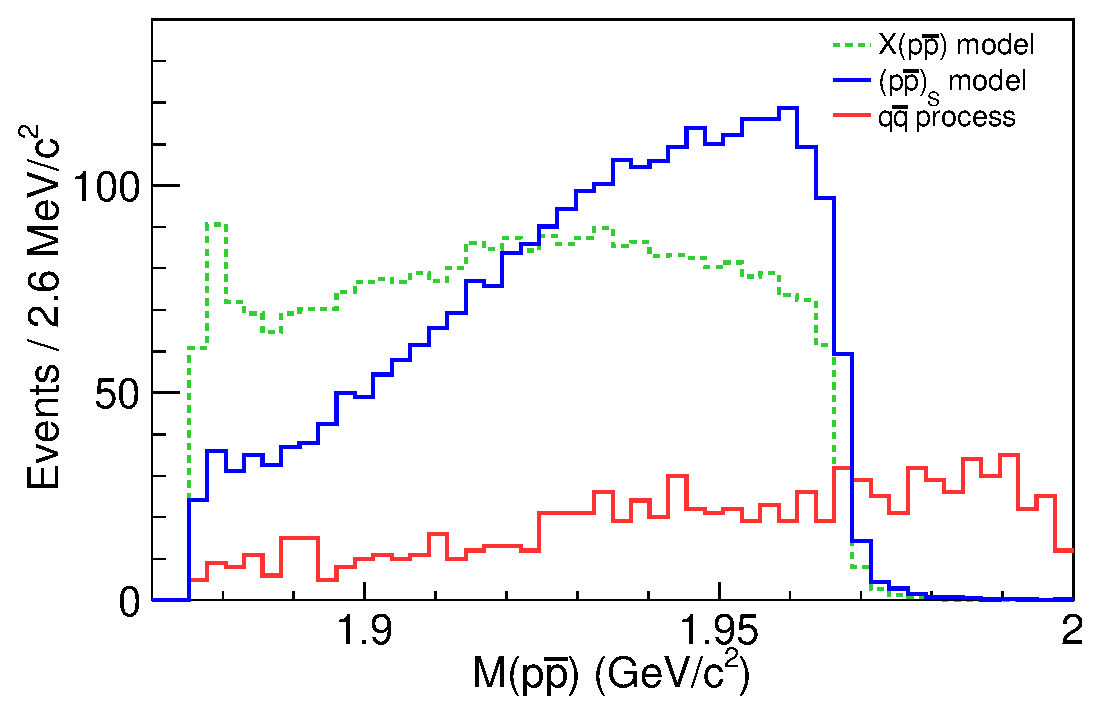
\includegraphics[width = 0.8 \linewidth]{dsToPPbar/mPP.eps}
    \caption{正反质子对的不变质量谱。
    绿色和红色的实线分别是信号和本底的形状。
    }\label{fig:mPP}
\end{figure}
如果在数据中的信号显著性小于3$\sigma$,本文则会为这个衰变道设一个上限。

\subsection{输入输出检查}
在正式分析真实的数据之间,做输入输出的检查是必要的。考虑到数据中只能
出现两种情况,要么有明显的信号,要么没有,因此本节分两种情况做检查,
首先考虑到可能看到信号,本文选择先从遍举 蒙特卡洛样本中随机抽样出和数据量
等同的子样本,并混入适当的信号蒙特卡洛样本,以此做输入输出检查。之后在遍举
MC子样本中不放任何信号,来研究实验的灵敏度。

\subsection{分支比的输入输出检查}
如上节所述,我们将把适当的信号蒙特卡洛样本混入遍举 MC之中来做分支比的
输入输出检查。信号道的分支比设为0.1\%,并利用\textbf{TRandom}从信号样本
中随机抽取相应个数的事例。类似的,
我们从混合样本中随机抽取与真实数据等大小的子样本。之后,利用同时拟合技术
去拟合上述操作得到的伪数据样本来获取分支比。更改随机数种子,重复以上操作,
便可以得到一系列的结果。
这这些结果中,某次的拟合结果如图~\ref{fig:total_fitting}示意。
实验上常常采取观察量\textbf{PULL}来衡量输入输出检查的好坏。若\textbf{PULL}
的中心值偏离0则意味了输出值有一定的偏差。
式\ref{eq:pull}定义了$\textbf{PULL}$,
\begin{equation}
    \label{eq:pull}
    PULL = \frac{\mu^{obs} -\mu_{0}}{\sigma_{\mu}^{obs}}
\end{equation}
式中$\mu^{obs}$和$\sigma_{\mu}^{obs}$分别是每次测量结果的中心值和误差,
$\mu_{0}$是输入值。在本节的输入输出检查中,$\mu$对应于信号
$D_{s}^{+} \to p\bar{p} e^{+} \nu_{e}$的分支比,$\mu_{0}$的取值是0.1\%。
本节多次实验得到的\textbf{PULL}分布如图\ref{Fig:pull_distribution}
所示。为了检验无偏性,这里用正态分布去拟合这个pull分布,拟合
结果见图\ref{Fig:pull_distribution},可以看出拟合结果没有明显的偏差。

\begin{figure}[htbp]
    \centering
    \begin{overpic}[width = 1.0\linewidth]{dsToPPbar/io/Catefit_mc.eps}
                \put(22, 26){\scalebox{0.80}{\color{juhong} (MC) } }
                \put(56, 26){\scalebox{0.80}{\color{juhong} (MC) } }
                \put(90, 26){\scalebox{0.80}{\color{juhong} (MC) } }
    \end{overpic}
        
    \caption{同时拟合三个标记道的结果。黑色的带误差棒的点代表伪数据,
    蓝线表示拟合的结果。红色和绿色的点虚线分别为信号和本底的形状。
    }%
    \label{fig:total_fitting}
\end{figure}


\begin{figure}[htbp]
    \centering
    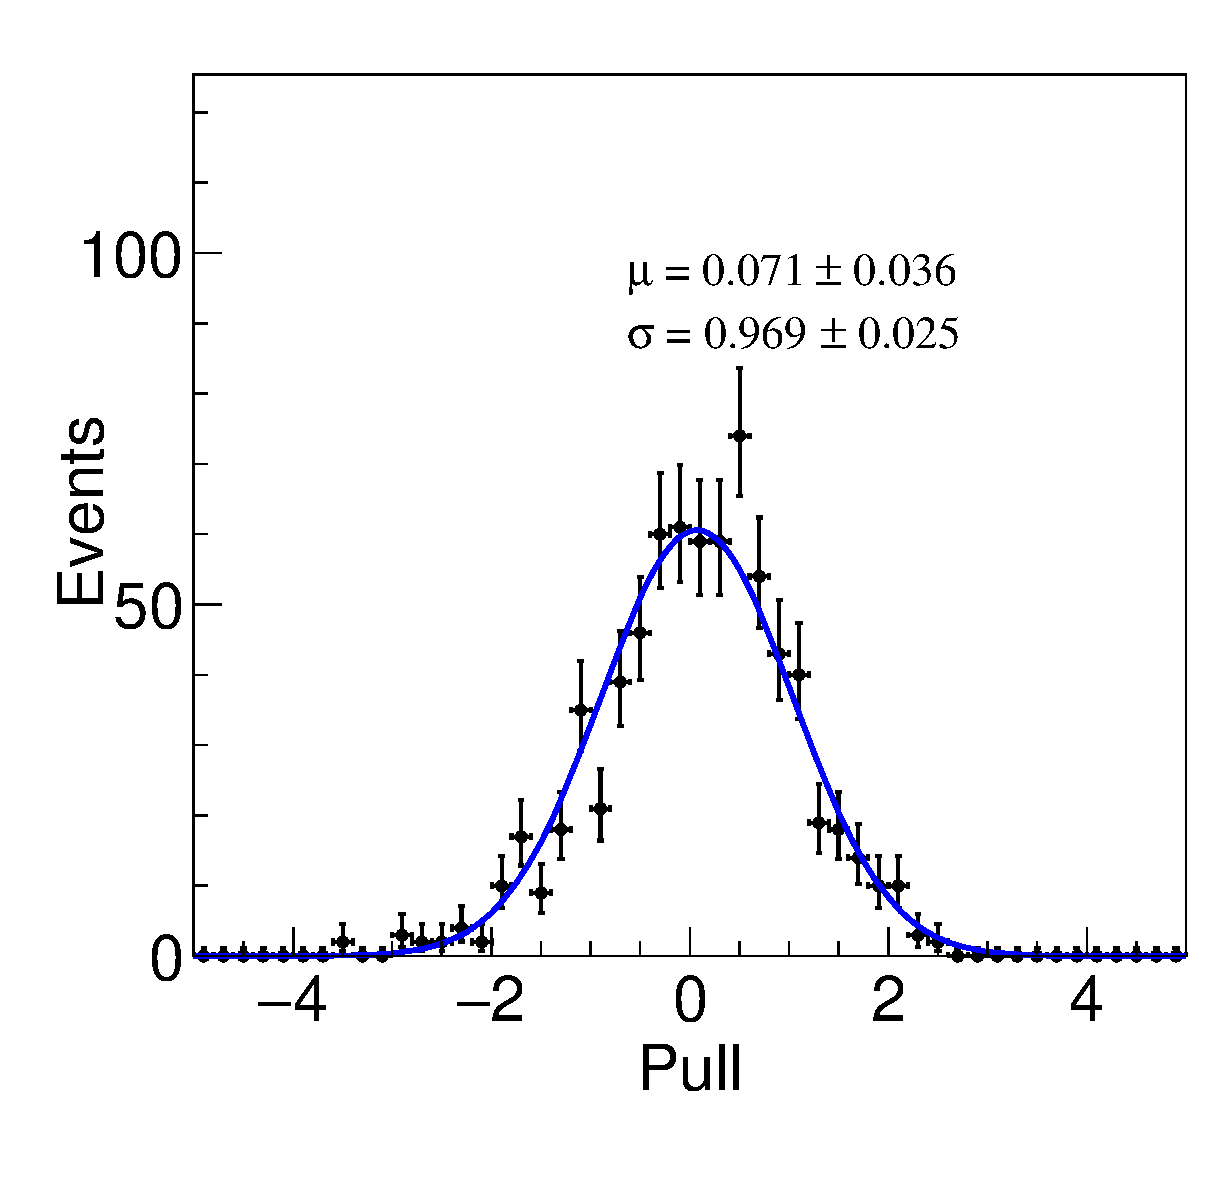
\includegraphics[width = 0.7\linewidth]{dsToPPbar/io/Pull_fit.eps}
    \caption{Pull分布,蓝线为高斯分布。
    }\label{Fig:pull_distribution}
\end{figure}

\subsection{信号灵敏度}
\subsubsection*{$\mathcal{B}(D_{S}^{+} \rightarrow p
\bar{p} e^{+} \nu_{e})$的灵敏度}\label{sec:UL_ds_ppbarenu_MC}
在本节,信号的分支比设为0,也就是伪数据中没有混入任何信号样本。基于同样的
拟合程序来处理这个伪数据,并按96\%的置信度水平设置衰变分支比的上限。
设上限的方法基于贝叶斯
统计\cite{Bayes2001An, Kendall2004Kendall, Zhu2007Upper},方法的精神简述如下:
当观测事例数$N$,分支比的概率分布为\ref{Equ:Bayes}
\begin{equation}
    \label{Equ:Bayes}
    p(B|N) = \frac{\mathcal{L} (N|B) }{\int \mathcal{L} (N|B_{0}) dB_{0}}
\end{equation}
式中$N$经过事例挑选程序后的事例数,$B$为信号的分支比。
注意到$\mathcal{L}(N|B)$的意义就是固定$B$之后通过拟合程序得到似然值,
因此固定分支比,并让其大小从0到1 变化,并通过方程\ref{Equ:Upperlimit}
来得到分支比的上限$Br^{up}$。
\begin{equation}
    \label{Equ:Upperlimit}
    \int^{upper~limit}_{0}p(B|N)dB = 0.9
\end{equation}

拟合的结果见图~\ref{fig:Catefit_mc_up},相应的分支比大小为
$(2.9 \pm 4.2)\times 10^{-5}$,没有显著性的信号,符合我们的预期,从而
按置信度90\%得到分支比的上限为$(1.36 \times 10^{-4})$ 。
\begin{figure}[htbp]
    \centering
    \begin{overpic}[width = 1.0 \linewidth]{dsToPPbar/io/Catefit_mc_up.eps}
        \put(23, 26) {\scalebox{0.9}{\color{juhong} (MC) } }
        \put(57, 26) {\scalebox{0.9}{\color{juhong} (MC) } }
        \put(91, 26) {\scalebox{0.9}{\color{juhong} (MC) } }
    \end{overpic}
    \caption{拟合伪数据中
        $D_{s}^{-}$不变质量谱的结果。其中蓝色的实线表示总的拟合结果,
        黑色的带误差棒的点代表伪数据,红色的点虚线是信号形状。
        }\label{fig:Catefit_mc_up}
\end{figure}


\begin{figure}[htbp] % upper limit Ds->ppbar enu
    \centering
    \begin{overpic}[width = 0.9 \linewidth]{dsToPPbar/io/UP_2DFit.eps}
        \put(68, 58) {\scalebox{1.2}{\color{juhong} (MC)}}
    \end{overpic}
    \caption{变动分支比得到的似然函数曲线。
    }\label{fig:upperlimit_遍举}
\end{figure}


\subsubsection*{研究$\mathcal{B}(D_{S} \rightarrow
X(p\bar{p}) e^{+} \nu_{e}, X \rightarrow p \bar{p})$的上限}
分析的一个重要的动机是研究$p\bar{p}$的共振态。本小节通过研究的
$\mathcal{B}(D_{s}^{+} \to X(p\bar{p}) e^{+} \nu_{e})$
上限来获取数据中探测共振态$X(p\bar{p})$的敏感度。研究基于遍举 蒙特卡洛样本,
通过联合$M(D_{s}^{-})$和$M(p\bar{p})$进行二维拟合得到信号数,进而确定
分支比或者其上限。
在这个二维拟合过程中,信号
蒙特卡洛样本的形状仍然用模拟形状来描述,其中$X(p\bar{p})$的宽度和质量的输入值分别为
1834 MeV$/c^{2}$ and 68 MeV。同时拟合三个标记道的结果如图\ref{fig:UP_D_Xenu}
所示。同样的,我们依旧可以考虑只对$M(D_{s}^{-})$进行拟合,
两者的主要区别为:
\begin{itemize}
    \item 一维拟合。为了得到衰变$D_{s}^{+} \to
        X(p\bar{p}) e^{+} \nu_{e}, X(p\bar{p}) \to p \bar{p}$的分支比上限,
        我们做了如下假设,所有的观测到的来自$D_{s}^{+}$的$p\bar{p}$对都是
        通过中间共振态$X(p\bar{p})$衰变而来。这样假设的合理性在于数据中没有
        明显的信号,故选择变动共振态的分支比扫描似然值获取上限,这就是假设的
        数学基础。故可以得到小结\ref{sec:UL_ds_ppbarenu_MC}同样的结果。
    \item 二维拟合。 这个方法能直接得到的$D_{s}^{+} \to
        X(p\bar{p})e^{+}\nu_{e},~X(p\bar{p})\to p\bar{p}$的分支比。由于
        二维分布能提供更多的数据,故我们期待二维拟合给出更高的灵敏度。
        分支比相应的在90\%置信度下的上限为$1.61 \times 10^{-4}$。总的拟合在
        $M(p\bar{p})$和$M(D_{s}^{-})$维度上的投影
        见图\ref{Fig:2Dfit}。通过变动分支比,得到的似然值曲线
        为\ref{fig:UP_D_Xenu}。
\end{itemize}


\begin{figure}
    \mbox{%
        \begin{overpic}[width = 7 cm]{dsToPPbar/io/mDs_total.eps}
            \put(71, 55) {\scalebox{0.9}{\color{juhong} (MC)}}
        \end{overpic}
        \begin{overpic}[width = 7 cm]{dsToPPbar/io/mPP_total.eps}
            \put(71, 55) {\scalebox{0.9}{\color{juhong} (MC)}}
        \end{overpic}
    }
    \caption{同时对三个标记道进行二维拟合的结果。
    蓝色的实线为总的拟合结果,红色的点虚线是信号形状,绿线分别是三个标记
    道的本底形状。
    }\label{Fig:2Dfit}
\end{figure}
\begin{figure}[htbp]
    \centering
    \mbox{%
        \begin{overpic}[width = 8 cm]{dsToPPbar/io/UP.eps}
            \put(67, 50) {\scalebox{1.2}{\color{juhong} (MC)}}
        \end{overpic}
    }
    \caption{从0开始变动分支比。图中的曲线为扫描得到的似然曲线,红色
    箭头的位置表示似然曲线总积分的90\%部分,也就是90\%置信度下分支比的上限。
        }\label{fig:UP_D_Xenu}
\end{figure}

两种方法结果的比较 
\begin{itemize}
    \item \textbf{上限}
        二维拟合能得到更低的上限,表现要稍优于一维拟合。两种方法得到的分支
        比上限分别是$1.61 \times 10^{-4}$、$1.64 \times 10^{-4}$。
    \item \textbf{系统误差}
        二维拟合的系统误差较大,增加了新的系统误差来源:共振态形状的
        不确定性包括$X(p\bar{p})$的质量和宽度、$B(X(p\bar{p})\to p\bar{p})$
        和本底形状的不确定性。
        与之相比,一维拟合的系统误差较小。
\end{itemize}
综合考虑,我们选择利用一维拟合$M(D_{S}^{-})$分布来决定信号产额或分支比上限。
\subsection{测量结果}\label{sec:result}
\subsubsection{信号产额}
在拟合的过程中,我们通过信号蒙特卡洛样本的形状卷积一个高斯分布以描述信号的形状,
高斯函数的参数,中心值和误差通过拟合单标记的$M(\Dsm)$来得到,
本底的形状则通过\textbf{RooKeyPdf}直接从混合蒙特卡洛样本中得到。
拟合的结果见图\ref{fig:data_Ds}。
\begin{figure}[htbp]
    \centering
        \begin{overpic}[width = 1.0 \linewidth]{dsToPPbar/Fit_Nom.eps}
            \put(21, 23){\scalebox{1.0}{\color{juhong} (data)} }
            \put(55, 23){\scalebox{1.0}{\color{juhong} (data)} }
            \put(90, 23){\scalebox{1.0}{\color{juhong} (data)} }
        \end{overpic}
    \caption{拟合$M(D_{s}^{-})$的结果。蓝色的实线为总的拟合结果,
    红色和绿色的点虚线分别为信号和本底的形状。
    }\label{fig:data_Ds}
\end{figure}
各个标记道中得到的信号数见表\ref{tab:data_yields},相应的分支比为
$( 5.0 ^{+ 6.3}_{-4.4} ) \times 10^{-5}$。
\begin{table}[htbp]
    \caption{各个标记道中拟合得到的信号数}\label{tab:data_yields}
    \begin{center}
        \begin{tabular} {p{0.5\linewidth} p{0.3\linewidth}}
            \toprule
            标记道 & 信号数 \\
            \midrule
            $K_{S}^{0}K^{-}$               & $0.3 ^{+0.4}_{-0.3}$ \\
            $K^{+} K^{-} \pi^{-}$          & $1.4 ^{+1.8}_{-1.3}$ \\
            $K_{S}^{0}K^{+}\pi^{-}\pi^{-}$ & $0.1 \pm 0.1$\\
            \bottomrule
        \end{tabular}
    \end{center}
\end{table}
\subsection{信号分支比的上限}
由于信号的显著性仅为1$\sigma$,本文将在显著性水平$90\%$对信号的分支比求上限。
求上限时,一个棘手的问题是如何处理系统误差。部分系统误差会直接影响拟合数据
时的似然函数,有些则是间接的。比如,本底形状的不确定性则会直接改变似然函数,
另一些因素,比如粒子鉴别的系统误差,则会通过影响信号数的估计间接的改变似然值。
本文利用文献\cite{K.Stenson:2006}的方法处理后者,将影响信号产额的系统误差吸收
到上限的估计之中。下面简要的叙述这一个方法,
通过拟合数据得到的似然值为$L(n)$,称之为原始似然函数,
接着通过卷积的方法吸收信号数的系统误差
如式~\ref{eq:smear}:
\begin{equation}
    \label{eq:smear}
    L(n)  = \int _{0} ^{1} L( n \cdot
    \frac{\epsilon}{\epsilon_{0}}) \
    e^{-\frac{{(\epsilon -  \epsilon_{0})}^{2}}
        {2 \sigma_{\epsilon}^{2}}
    } d \epsilon
\end{equation}
式中$\epsilon_{0}$是上文求得的双标记效率,
$\sigma_{\epsilon}$是效率的系统误差。
原始的似然曲线和经过卷积后的似然曲线见图~\ref{fig:prob},
通过积分求90\%的区间后便得到了分支比的上限
\begin{equation}
    \mathcal{B}(D_{s}^{+} \to p \bar{p} e^{+} \nu_{e}) < 1.92 \times
    10^{-4} \notag
\end{equation}

\begin{figure}[htbp]
    \centering
    \begin{overpic}[width = 0.8 \linewidth]{dsToPPbar/prob.eps}
        \put(67, 60){\scalebox{1.0}{\color{juhong} (data) }}
    \end{overpic}
    \caption{似然函数曲线。蓝色和红色和实线分别表示原始似然函数和卷积后
    的似然函数曲线。
    }\label{fig:prob}
\end{figure}



\subsection{系统误差研究}
本文分两种情况研究系统误差
\begin{itemize}
    \item \textbf{I}: 直接影响似然曲线, 比如本底形状;
    \item \textbf{II}: 间接影响似然曲线, 比如寻迹、粒子鉴别。
\end{itemize}
这两类系统误差有明显的不同,
第\textbf{II}类系统误差通过卷积高斯被吸收到上限的估计中,
但是第\textbf{I}类显然不能。

对第类系统误差的讨论见小节\ref{sec:deal_with_background},
比如本底形状系统误差的一个来源是\textbf{RooKeyPdf}类中一个参数``rho''的取值,
这里在1--4之间变动的``rho''的值,每种取值得到的上限列在表\ref{tab:vary_rho}
中。出于保守估计,本文选择其中最大的值作为上限。
\begin{table}[htbp]
    \caption{``rho''的取值对上限的影响。}%
    \label{tab:vary_rho}
    \begin{center}
        \begin{tabular} {c  c c c c c c c }
            \toprule 
            rho  &  1.0 & 1.5 & 2.0 & 2.5 & 3.0 & 3.5 & 4.0 \\
            \midrule  
            UL ($10^{-4}$) & 1.90 & 1.91 & 1.91 & 1.92 & 1.92 & 1.92
            &1.92 \\
            \bottomrule
        \end{tabular}
    \end{center}
\end{table}

\subsection{小结}
采用盲分析方法,本文对伪数据进行了充分研究,决定了实验方案和所有的事例选择
条件,最终选择观测量--$M(D_{s}^{-})$,作为决定信号产额的唯一观测量。
为了验证观测量的合理性,本节比较了两个方法--一维拟合与二维拟合,其中二维拟合
同时考虑了$M(D_{s}^{-})$和$M(p\bar{p})$。
综合考虑到灵敏度和系统误差,本文发现二维拟合对结果的提高极其有限但是又带来
了较大的系统误差,故本文坚持采用一维拟合的方案。
打开数据之后,测得信号的分支比为
$( 5.0 ^{+ 6.3}_{-4.4} ) \times 10^{-5}$,显著性不足3$\sigma$,考虑到
系统误差,在90\%的置信度下,本文给出为
$\mathcal{B}(D_{s}^{+} \to p \bar{p} e^{+} \nu_{e}) < 2.0\times
10^{-4}$。系统误差的具体研究将在下文给出。 

\section{系统误差的研究}%
\label{sec:Systematic_Uncertainties}
系统误差的来源可以分为四类:
\begin{itemize}
    \item 重建:
    质子的寻迹、质子的粒子鉴别;
    \item 事例选择条件:
        对$MM^{2}$, 质子动量,和电子动量的要求;
    \item 拟合:
        信号形状、本底形状、单标记$D_{s}^{-}$介子产额;
    \item 模型:
        产生子模型。
\end{itemize}

\subsection{重建}
单标记侧的寻迹和粒子鉴别的系统误差和双标记侧的相互抵消,因此重建的系统误差
只有信号侧的质子寻迹和鉴别的系统误差。质子的粒子鉴别的系统误差在
小节~\ref{Sec:Correction_of_Efficiency}已经进行了研究,系统误差的大小为
2.2\%。
对于质子寻迹的系统误差,本文利用数据和伪数据中的质子寻迹效率,对信号蒙特卡洛样本进行加权
平均,所用到的公式是~\ref{eq:track-error},
\begin{equation}
    \begin{aligned}
        \label{eq:track-error}
        &\epsilon(reweight) = \sum_{i}  \frac{n_{i} \epsilon_{i}(data) / 
        \epsilon_{i} (MC) }{N} \notag  \\
        & \delta_{i}  =  \frac{\epsilon_{i}(data) -
        \epsilon(MC)}{\epsilon_{i}(data)}  \notag  \\
        &\bar{\delta}  =  \frac{\epsilon(reweight) -
        \epsilon(MC)}
        {\epsilon (reweight)}
    \end{aligned}
\end{equation}
式中$\epsilon_{i}(data)$和
$\epsilon_{i}(MC)$分别是数据和伪数据 
中质子的寻迹效率,本文采用文献~\cite{HaoXq:ProtonPID}中的结果,
相应的大小列在表~\ref{tab:proton-efficiency}之中,
$\epsilon(reweight)$则是经过加权后的信号效率。
信号蒙特卡洛样本按正反质子的动量大小分成$5\times5$个区间,
如表~\ref{tab:ratios}所示。\ref{tab:evts}. 
在下面的分析中,将按这25个区间进行加权得到总效率,进而决定质子寻迹的系统
误差。首先考虑到第$i$个区间内的效率等于
\begin{equation}
    \epsilon_{i}(p\bar{p}) = \epsilon_{n}(p) \epsilon_{m}(\bar{p})
    \notag
\end{equation}
式中质子在$n$个动量区间,反质子则在$m$个动量区间,这一个区间内的
同时寻找到正反质子对的效率为$\epsilon_{i}(P\bar{P})$。
在之后的公式里,脚标$p\bar{p}$将被省略。
\begin{table}[htbp] %efficiency
    \caption{数据和蒙特卡洛样本中的质子寻迹效率差异。
    }%
    \label{tab:proton-efficiency}
    \begin{center}
        \begin{tabular} {c c c c c c}
            \toprule
            $p_{t}(p) (MeV)$  &  100--200 & 200--300 & 300--400 
            & 400--500 & 500--600 \\
            \midrule
            $1-  \frac{\epsilon_{MC}}{\epsilon_{data}}  (\%) $  &
            $ -2.3 \pm  2.4  $ & $ -0.27 \pm 1.1  $  &
            $ -0.34 \pm 0.42 $ & $ - 0.28 \pm 0.32 $ & 
            $ -0.09 \pm 3.7 $  \\
            \midrule
            $p_{t}(\bar{P}) (MeV)$  &  100--200 & 200--300 
            & 300--400 & 400--500 & 500--600 \\
            \midrule
            $1-  \frac{\epsilon_{MC}}{\epsilon_{data}} (\%)$  &
            $ -7.6 \pm  5.3  $ & $ -0.96 \pm 1.3  $  &
            $ -0.36 \pm 1.1 $ & $ - 1.2 \pm 1.2 $ & 
            $ -0.6 \pm 2.6 $ \\
            \bottomrule
        \end{tabular}
    \end{center}
\end{table}
\begin{table}[htbp] %ratio
    \caption{每个区间内事例数比例。按质子(反质子)的动量划分区间。
    信号蒙特卡洛样本总大小为35000个事例。}%
    \label{tab:ratios}
    \centering
    \begin{tabular} {c  c |  c c  c c c}
        \toprule
        \multicolumn{2}{c}{\multirow{2}{*}{$\frac{n_{i}}{N}$~(\%)}}
        & \multicolumn{5}{|c}{$p_{t}(\bar{P}) (MeV)$} \\ 
        & &  100--200 & 200--300 & 300--400 & 400--500 & 500--600 \\
        \midrule
        \multirow{5}{*}
        {\rotatebox{90}{$p_{t}(\bar{P}) (MeV)$ }} 
        &  100--200 & 1.34  & 7.79  & 3.64 & 0.48 & 0.011 \\
        & 200--300      & 8.84  & 38.9  & 13.4 & 1.48 & 0.008 \\
        & 300--400      & 4.49  & 13.7  & 3.38 & 0.149 & 0.00 \\
        &400--500     & 0.625 & 1.62  & 1.18 & 0.00 & 0.00 \\
        &500--600      & 0.008 & 0.011 & 0.00 & 0.00 & 0.00 \\
        \bottomrule
    \end{tabular}
    \begin{tabular} {c  c |  c c  c c c}
        \toprule
        \multicolumn{2}{c}{\multirow{2}{*}{$n_{i}$}}
        & \multicolumn{5}{|c}{$p_{t}(\bar{P}) (MeV)$} \\ 
        & &  100--200 & 200--300 & 300--400 & 400--500 & 500--600 \\
        \midrule
        \multirow{5}{*}
        {\rotatebox{90}{$p_{t}(\bar{P}) (MeV)$}} 
        & 100--200 & 475  & 2764  & 1292 & 172 & 4 \\
        & 200--300 & 3138 & 13814 & 4743 & 526  & 3 \\
        & 300--400 & 1594 & 4873  & 1198 & 53 & 0 \\
        & 400--500 & 222  & 574   & 42   & 0  & 0 \\
        & 500--600 & 3    & 4     & 0 & 0  & 0 \\
        \bottomrule
    \end{tabular}
\end{table}

综上所述,可以得到 
\begin{equation}
    \bar{\delta} = 1.2 \% \notag
\end{equation}
$\bar{\delta}$的误差由方程\ref{eq:track-corr-error}得到
\begin{equation}
    \begin{aligned}
        \label{eq:track-corr-error}
        \Delta \bar{\delta }^{2} & = 
        \sum_{i,j} 
        \frac{\partial \bar{\delta }} {\partial \delta_{i}} \cdot 
        \frac{\partial \bar{\delta }} {\partial \delta_{j}} \cdot 
        \delta_{i} \delta_{j}  
        \notag \\
        &= \sum_{i,j}  \frac{n_{i}}{N} \frac{n_{j}}{N}
        cov_{i,j}   \Delta  \delta_{i} \Delta  \delta_{j} 
    \end{aligned}
\end{equation}
式中$cov_{i,j}$是$\delta_{i}$和$\delta_{j}$的相关系数。
如果假设$cov_{i,j}=0$,也就是各个区间内的样本相互独立将得到
$ \Delta \bar{\delta } = 1.0\%$;如果做最保守的估计,假设各个区间
之间完全相关,也就是$cov_{i,j}=1$,那么将得到较大的误差,大小为 
\begin{equation}
    \Delta \bar{\delta} = 2.9\% \notag
\end{equation}
因此出于保守估计,这项系统误差定为2.9\%.

\subsubsection{电子寻迹}
在这些分析中,电子寻迹的系统误差为0。按前文所述,只有找到一对正反
质子对之后才考虑寻找电子的径迹。不管是否能够找到电子的径迹,这个事例
都将被保留,因此电子寻迹不会贡献任何系统误差。

\subsection{事例选择条件}
由于仅有约5\%是事例中能够找到电子径迹,在这部分事例中,本文要求电子的动量
小于90MeV,带来的系统误差约为1\%,对总的事例的系统误差的贡献可以忽略不记。
除了对电子动量的选择条件,本文还要求
丢失不变质量大于0${(GeV/c^{2})}^{2}$,这项系统误差的来源在于数据和蒙特卡洛样本之间
的$MM^{2}$的分辨率不同。分辨率由带电径迹的
探测器分辨决定。为了补偿这种差异,本文选择在蒙特卡洛信号形状的基础上卷积一个高斯
函数来描述数据中的$MM^{2}$形状,高斯函数参数的不确定性带来的相对变化
作为系统误差,在章节\ref{sec:cut-on-MM}中做了详细研究,系统误差定为1.0\%。

\subsection{拟合方法}
和单标记道有关的系统误差包括:信号形状、本底形状和拟合范围。
为了估计信号形状带来的系统误差,本文变动拟合模型中的信号形状,
从模拟形状变为双高斯函数,信号产额仅仅变化0.5\%,因此本文选择把0.5\%作为
信号形状带来的系统误差。同样的,本文变化本底形状,用更高阶的切比雪夫多
项式替代模型中的本底形状,并信号产额的变化作为系统误差。
为了保守估计拟合范围带来的系统误差,本文5MeV的范围内浮动拟合范围的上下限,
信号产额的最大变化作为系统误差。
这三项系统误差的大小总结在表\ref{tab:sys-uncerainty-fitting}中。

\begin{table}[htbp]
    \caption{来自拟合的系统误差}%
    \label{tab:sys-uncerainty-fitting}
    \centering
    \begin{tabular}{p{0.2 \linewidth} p{0.2 \linewidth} p{0.2 \linewidth} 
        p{0.2 \linewidth}}
        \toprule
        误差来源 & 拟合范围 & 本底形状 & 信号形状\\
        \midrule
        误差大小 & 0.3\%  & 0.2\%  & 0.5 \%  \\ 
        \bottomrule
    \end{tabular}
\end{table}
这三项系统误差总和为0.7\%。
\subsection{产生子模型}
在正则模型里,本文假定$D_{s}^{+}$介子直接衰变到
$p\bar{p}e^{+} \nu_{e}$, 产生的$p\bar{p}$对形成S波。
另外,还有很多其他的合理的模型,比如
$p\bar{p}$可能来自中间共振态$X(p\bar{p})$,假定我赝标量粒子,宽度和质量
分别为
1834 MeV$/c^{2}$、68 MeV。两个模型中的信号效率的相对差异为$18\%$。
此外中间共振态的宽度和质量也会影响效率,在小节\ref{uncertainties for Xpp}
中详细地研究了这项系统误差,
约为2.5\%

\subsection{本底}%
\label{sec:deal_with_background}
在获取上限的过程中,本底带来的系统误差不能简单的通过公式~\ref{eq:smear}
吸收到上限的估计之中。如果变动本底的形状,将会得到一系列上限的估计值。
下文将详细叙述本底形状的变化方式。在小结\ref{sec:dt-efficiency}中,
本底形状借助于工具\textbf{RooKeyPdf}得到,最大的确定性来自参数``rho''
的设置值,本文把``rho''在1--4之间浮动,将得到一系列形状,接着根据每种
形状估计分支比上限,并把最大的上限估计值作为最终的实验结果。

\subsection*{系统误差研究的总结}
至此,本文已经研究了所有的系统误差,每项系统误差的具体数值列在
表\ref{tab:short_summary}中。

\begin{table}[htbp]
    \caption{系统误差的总结}%
    \label{tab:short_summary}
    \centering
    \begin{tabular}{p{0.45 \linewidth} p{0.45 \linewidth} }
        \toprule
        来源 & 误差 ($\%$) \\ 
        \midrule
        单标记产额       & 1.0 \\
        寻迹$^{a}$       & 2.9 \\
        粒子鉴别         & 2.2 \\
        对$MM^{2}$的要求 & 1.0 \\
        产生子模型$^{b}$ & 18 \\
        \midrule
        总和 & 19 \\
        \bottomrule
    \end{tabular}
\end{table}


% ====================================================
%   Copyright (C)2019 All rights reserved.
%
%   Author        : Xin-Xin Ma
%   Email         : xxmawhu@163.com
%   File Name     : spinPrece.tex
%   Last Modified : 2020-01-16 16:37
%   Describe      :
%
% ====================================================%
\chapter{研究超子在磁场中的进动效应}
\section{简介}%
本章节我们将研究超子对的产生特点。以$e^{+}e^{-} \to J/\psi \to \Lambda \bar{\Lambda}$为例做研究,
这是因为这个过程受到了广泛关注,并且过程简单又能够有效的说明问题。
考虑到$\Lambda$ ($\bar{\Lambda}$)具有一定的磁矩,因此其自旋方向受磁场的影响。北京谱仪内部恰好有
一个强度为1T的磁场,故推断$\Lambda$ ($\bar{\Lambda}$)的自旋方向将会绕着磁场做转动,这意味
着$\Lambda$ ($\bar{\Lambda}$)衰变时刻的自旋方向将不同于产生时刻的,这将导致整体末态角分布发生变化。
然而实验上\cite{Ablikim:2018zay, Ireland:2019uja, Ablikim:2017tys,
Ablikim:2005cda,Aubert:2007uf, Ablikim:2012bw, Aubert:2009am}都忽略了这一点差异,这会对实验结果造成潜在的测量偏差。在下面的小节里,
我们首先给出讨论实验上所用的角分布,并给出修正项,接着进行实验模拟以定量的研究忽略修正项带来测量偏差。

\section{实验研究现状}
在北京谱仪采集到的十三亿$J/\psi$的样本的基础上,合作组对
$\Lambda$的衰变参数$\alpha_{-}$进行了最精确的测量,实验结果为 $0.750 \pm 0.009 \pm 0.004$~\cite{Ablikim:2018zay},
出乎意料的和世界平均测量值偏离了7$\sigma$,这修正了一系列的实验测量结果。
在2019年,文献\cite{Ireland:2019uja}利用CLAS的数据重新测量了$\alpha_{-}$,结果和BESIII的偏离为2$\sigma$。
目前这两个实验都没有考虑到$\Lambda$在磁场中的进动,这也是本章研究的一个出发点。以北京谱仪为例,
考虑到束流能量和$\Lambda$的寿命,很容易得到$\Lambda$在探测器内部的平均飞行距离为12cm,相应的进动角约
为1$^o$。进动的角度虽然小,但是实验的精度很高。在实验\cite{Holmstrom:2004ar}中对$\Xi^{-}$的$CP$破坏测量
精度已经达到了$10^{-4}$,在未来的超级粲-陶工厂中,对超子衰变$CP$破坏的灵敏度将达到$10^{-4}$
到$10^{-5}$\cite{Bigi:2017eni},在这种精度下,忽略磁场带来的进动将是致命的。

\section{$\Lambda\bar{\Lambda}$对的产生}
在北京谱仪上,相干的$\Lambda \bar{\Lambda}$通过级联过程$e^+e^- \to J/\psi \to \Lambda \bar{\Lambda}$产生。
有效振幅为
\begin{equation}
    \begin{split}
        M &= \frac{ie^2}{q^{2}} j_{\mu} \bar{u}(p_{1}, s_1) \left( F^H_1(q^2) \gamma_{\mu} +
        \frac{F^H_2(q^2)}{2m_{\Lambda}} p_{\nu} \sigma^{\nu\mu}  \gamma_5 \right) \\
        & \times \nu(p_2, s_2),
    \end{split}
\end{equation}
式中的$p_1$ ($p_2$)表示$\Lambda$ ($\bar{\Lambda}$)的动量, 
$m_{\Lambda}$是$\Lambda$的质量,$s_1$ ($s_2$)为$\Lambda$ ($\bar{\Lambda}$)的自旋矢量, 
转移动量$q = p_{1} + p_{2}$, $p = p_{1} - p_{2}$, $s = p^{2}$,
$j_{\mu} = \bar{u}(k_1) \gamma_{\mu} \nu(k_2)$是轻子流其中的$k_{1}$ ($k_{2}$)
是$e^{-}$ ($e^{+}$)的动量。 
需要特别指出的是形状因子$G^H_{E}$和$G^H_{M}$即所谓的强形状因子\cite{Faldt:2016qee},
这是由于$\Lambda\bar{\Lambda}$是通过$J/\psi$的强衰变产生的\cite{Faldt:2017kgy},与之相关的常用的
形式$F^H_{1,2}$的定义为
\begin{equation}
    G^H_{M} = F^H_1 + F^H_2,~G^H_{E} = F^H_1 + \tau F^H_2,
\end{equation}
其中$\tau = \frac{q^2}{4 m_{\Lambda}^2}$。
仿照文献\cite{Dubnickova:1992ii,Gakh:2005hh,Czyz:2007wi}的方法,很容易得到微分截面为(丢掉了和角分布无关的常数):
\begin{equation}
\label{eq:jpsi_LL}
    \begin{split}
        \frac{d\sigma}{d \cos\theta}  \sim & 1+ \alpha _{\psi } \cos^2\theta
        + \sin ^2\theta \hat{s}_{1}^x \hat{s}_{2}^x
        + \alpha_{\psi} \sin^2\theta \hat{s}_{1}^y \hat{s}_{2}^y \\
        &- \left( \alpha_{\psi} +\cos^2 \theta  \right)\hat{s}_{1}^z \hat{s}_{2}^z
        + \sqrt{1-\alpha_{\psi}^2} \cos\Phi  \sin\theta \\
        & \times    \cos\theta
        \left( \hat{s}_{1}^x \hat{s}_{2}^z  - \hat{s}_{1}^z \hat{s}_{2}^x\right)
        +\sqrt{1-\alpha _{\psi}^2}
        \sin\Phi  \sin\theta \\
        & \times \cos\theta  (\hat{s}_{1}^y - \hat{s}_{2}^y),
    \end{split}
\end{equation}
式中的$\theta$是$e^{+}$和$\Lambda$飞行方向之间的夹角,
$\alpha_{\psi} = \frac{\tau |G_{M}|^{2} -  |G_{E}|^{2}}{\tau |G_{M}|^{2} + |G_{E}|^{2}}$,
$\hat{s}^{i}_1$ ($\hat{s}^{i}_2$) 是$\Lambda$ ($\bar{\Lambda}$) 在其母粒子质心系下的
自旋的方向的第$i$个分量(选择$\Lambda$ ($\bar{\Lambda}$)动量方向作为Z轴,
$\vec{p}_1 \times \vec{k}_2$ ($\vec{p}_2 \times \vec{k}_2$)作为Y轴)。
$\Phi$是两个形状因子之间的相位差,定义为
\begin{equation}
    \frac{G^H_{E}}{G^H_{M}} = e^{i \Phi} \left|\frac{G^H_{E}}{G^H_{M}} \right |.
\end{equation}

\section{$\Lambda$自旋方向的改变}
与实验\cite{Ablikim:2018zay}有所不同的是,我们根据外部的磁场大小计算了衰变时刻的自旋取向。
考虑到自旋转动角度较小,利用$\Lambda$磁矩与磁场的相互作用\cite{Sakurai:2011zz},可以得到:
\begin{equation}
\label{eq:retate-s-sp}
    \hat{s}'_{1} = \hat{s}_{1} + \omega \tau_{\Lambda} \hat{B}  \times
    \hat{s}_{1},
\end{equation}
式中$\hat{s}'_{1}$代表$\Lambda$在其质心系下的衰变时刻$\tau_{\Lambda}$的自旋取向,并把
$\Lambda$产生的时刻作为时间起始点,$\hat{B}$是在$\Lambda$质心系下的探测器磁场的方向,
$\omega$是$\Lambda$的自旋绕磁场转动的频率,这个频率依赖于磁场强度$B$和$\Lambda$的磁矩大小$\mu_{\Lambda}$,
关系为
\begin{equation}
    \omega  = - \frac{2 \mu_{\Lambda} B}{\hbar},
\end{equation}
如果取$\mu_{\Lambda} = -0.613 \pm 0.04 \mu_{N}$~\cite{PDG},$B=1T$,$\Lambda$的平均寿命
$\tau_{\Lambda} = 2.632 \times 10^{-10}$ s及其典型动量大小为1 GeV/$c$,那么容易计算得到进动角度大约
为$\mathcal{A}_{\rm rota} = \omega \tau_{\Lambda} =0.017$ rad,类似的可以计算出其他的长寿命的超子,
比如$\Xi$, $\Omega$, $\Sigma^{\pm}$等在磁场中进动的角度。

一旦正确的认识到$\Lambda$衰变时刻的自旋取向为$\hat{s}'_{1}$,就能写出过程$\Lambda \to p \pi^-$的振幅:
\begin{equation}
    |M_{1}|^{2} \sim 1 + \alpha_{-} \hat{s}'_{1} \cdot n_{p},
\end{equation}
式中的$n_p$是质子在$\Lambda$质心系下的飞行方向,$\alpha_{-}$就是$\Lambda$的衰变参数,
类似的$\alpha_{+}$是$\bar{\Lambda}$的相应的衰变参数,与之相关的常见的一种$CP$不对称观测量
为$A_{CP} = \frac{\alpha_{-} + \alpha_{+}}{\alpha_{-}- \alpha_{+}}$。 最近的$A_{CP}$测量的实验结果为:
$A_{CP} = -0.006 \pm 0.012 \pm 0.007$\cite{Ablikim:2018zay},  而基于标准模型的理论
预言的量级为$10^{-5}$\cite{Donoghue:1986hh, Tandean:2002vy}。

为了得到整体的微分截面,我们需要给出$\hat{s}_{1}$, $\hat{s}'_{1}$的具体变换关系,
考虑到欧拉转动矩阵元,可以将方程\ref{eq:retate-s-sp}展开为
\begin{equation}
    \left(
    \begin{array} {c}
        \hat{s}'^x_{1} \\
        \hat{s}'^y_{1} \\
        \hat{s}'^z_{1} \\
    \end{array}\right)
    =
    \left(%
    \begin{array}{ccc}
        1                       & - \mathcal{A}_{\rm rota} \hat{B}'_{z}  & \mathcal{A}_{\rm rota} \hat{B}'_{y}  \\
        \mathcal{A}_{\rm rota}  \hat{B}'_{z}  & 1                       & -\mathcal{A}_{\rm rota}\hat{B}'_{x} \\
        -\mathcal{A}_{\rm rota} \hat{B}'_{y} & \mathcal{A}_{\rm rota}   \hat{B}'_{x} & 1                      \\
    \end{array}
    \right)
    \left(%
    \begin{array} {c}
        \hat{s}^x_{1} \\
        \hat{s}^y_{1} \\
        \hat{s}^z_{1} \\
    \end{array}\right),
\end{equation}
这里的$n_{\Lambda}$ 代表$\Lambda$在$J/\psi$的静止系下的运动方向,$\hat{B}'=\hat{B} + (\gamma-1) (\hat{B} \cdot n_{\Lambda}) n_{\Lambda}  $为将探测器内的磁场$B$通过洛伦兹变换在$\Lambda$静止系下的大小\cite{landau1952the}。
\section{修正后的微分散射截面}
当对$\Lambda$的自旋求和时,需要运用其正交性,即
\begin{equation}
    <\hat{s}^{i} \hat{s}^{j} > = \delta^{ij}
\end{equation}
这样很容易求得总的微分散射振幅:
\begin{equation}
    |M_{\rm total}|{}^{2} = |M\left(J/\psi \to\Lambda \bar{\Lambda} \right)|^{2} 
                       \cdot |M\left(\Lambda \to \pi^{-} p\right)|^{2}
                       \cdot |M\left(\bar{\Lambda} \to \pi^{+} \bar{p}\right)|^{2}
\end{equation}
在这里考虑到$\Lambda$的寿命很长在探测器内部的磁场中已经迅速退相干,故采取振幅的模相乘的形式。
我们使用一个技巧来得到整体的微分截面,由于自旋的正交性,
考虑到$|M\left(\Lambda \to \pi^{-} p\right)|^{2}$的形式及自旋的变换关系,
我们只需要将\ref{eq:jpsi_LL}中的$(s_1^{x}, s_1^{y}, s_1^{z})$替换为
\begin{equation}
    \left(
    \begin{array}{ccc}
        1                        & \mathcal{A}_{\rm rota} \hat{B}'_{z}     & -\mathcal{A}_{\rm rota} \hat{B}'_{y} \\
        - \mathcal{A}_{\rm rota}  \hat{B}'_{z} & 1                         
        & \mathcal{A}_{\rm rota} \hat{B}'_{x}  \\
        \mathcal{A}_{\rm rota} \hat{B}'_{y}    & - \mathcal{A}_{\rm rota}  \hat{B}'_{x} & 1                      
    \end{array}
    \right)
    \left(%
    \begin{array} {c}
        \alpha_{-} n^x _{p} \\
        \alpha_{-}  n^y_{p} \\
        \alpha_{-}  n^z_{p} 
    \end{array}
    \right),
\end{equation}
对$s_2$做同样的处理即可, 于是得到微分总截面为:
\begin{equation}
    \label{eq:pdf}
    \begin{split}
        &\frac{d\sigma}{d \cos\theta d\Omega_{1} d\Omega_{2}}
        \sim  1+ \alpha _{\psi } \cos^2\theta
        + \sin ^2\theta \alpha_- \alpha_+ n_{p}^{x} n_{\bar{p}}^x
        + \alpha_{\psi}  \alpha_{-}  \\
        & \times \alpha_{+} \sin^2\theta
        n_{p}^y n_{\bar{p}}^y 
        - \left( \alpha_{\psi} +\cos^2 \theta  \right) \alpha_- \alpha_+ 
        n_{p}^z n_{\bar{p}}^z
        + \sqrt{1-\alpha_{\psi}^2}  \\
        & \times \alpha_- \alpha_+  \cos\Phi  \sin\theta
        \cos\theta 
        \left( n_{p}^x n_{\bar{p}}^z  - n_{p}^z n_{\bar{p}}^x\right)
        +\sqrt{1-\alpha _{\psi}^2} \sin\Phi\\ 
        & \times   \sin\theta \cos\theta  
        (\alpha_- n_{p}^y - \alpha_+ n_{\bar{p}}^y)
        + \alpha _- \alpha _+ \mathcal{A}_{\rm rota}  \sin ^2\theta
        \left(\hat{B}'_z \left(\hat{n}_{\bar{p}}^x
        \hat{n}_{p}^y \right. \right.  \\
        & \left. \left. -\hat{n}_{p}^x \hat{n}_{\bar{p}}^y\right)-\hat{B}'_y
        \left(\hat{n}_{p}^x \hat{n}_{\bar{p}}^z+\hat{n}_{\bar{p}}^x
        \hat{n}_{p}^z\right)\right)
        + \alpha_{\psi}
        \alpha _- \alpha _+ \mathcal{A}_{\rm rota} \sin^2\theta 
        \\ & \times \left(-\hat{B}'_z \hat{n}_{p}^x
        \hat{n}_{\bar{p}}^y+\hat{B}'_z \hat{n}_{\bar{p}}^x \hat{n}_{p}^y-\hat{B}'_x
        \hat{n}_{p}^y \hat{n}_{\bar{p}}^z+\hat{B}'_x \hat{n}_{\bar{p}}^y
        \hat{n}_{p}^z\right)
        - \alpha _+  \alpha _- \mathcal{A}_{\rm rota} 
        \\ & \times   \left( \alpha_{\psi} +\cos^2 \theta  \right)
        \big(\hat{B}'_y \hat{n}_{p}^x
        \hat{n}_{\bar{p}}^z
        -\hat{B}'_x \hat{n}_{p}^y \hat{n}_{\bar{p}}^z
        +\hat{B}'_y
        \hat{n}_{\bar{p}}^x \hat{n}_{p}^z+\hat{B}'_x \hat{n}_{\bar{p}}^y
        \hat{n}_{p}^z \big)
        \\ & + \mathcal{A}_{\rm rota}  \alpha _- \alpha _+ \sqrt{1-\alpha_{\psi}^2} \cos\Phi  \sin\theta
        \cos\theta \Big(\hat{B}'_x \hat{n}_{p}^x
        \hat{n}_{\bar{p}}^y+\hat{B}'_x \hat{n}_{\bar{p}}^x \hat{n}_{p}^y
        \\ &
        +\hat{B}'_z
        \hat{n}_{p}^y \hat{n}_{\bar{p}}^z
        +\hat{B}'_z \hat{n}_{\bar{p}}^y
        \hat{n}_{p}^z\Big)
        + \mathcal{A}_{\rm rota} \sqrt{1-\alpha _{\psi}^2}
        \sin\Phi  \sin\theta \cos\theta    \\
        & \times \left(
        \alpha_+ \hat{B}'_x \hat{n}_{\bar{p}}^z
        -\alpha _- \hat{B}'_z \hat{n}_{p}^x+\alpha _-
        \hat{B}'_x \hat{n}_{p}^z
        - \alpha _+ \hat{B}'_z \hat{n}_{\bar{p}}^x
        \right)
        ,
    \end{split}
\end{equation}
这里的$\Omega_{1,2}$表示质子(反质子)在$\Lambda$($\bar{\Lambda}$)静止系下的立体角。
值得注意的是,$\Lambda$的极化状态发生了变化,
\begin{equation}
    \begin{aligned}
        P_{\Lambda}^{x} & = - \mathcal{A}_{\rm rota} \hat{B}'_{z} P_{\Lambda}^{y} \\
        P_{\Lambda}^{z} & =  \mathcal{A}_{\rm rota} \hat{B}'_{x}
        P_{\Lambda}^{y},  
    \end{aligned}
\end{equation}

这里的$P_{\Lambda}^{x,y,z}$表示极化矢量在$x$, $y$ 和 $z$轴方向的投影。如果没有外磁场,
那么$\Lambda$在$x$和 $z$方向的极化都应为0。以 $P_{\Lambda}^{x}$为例,有无磁场的极化分布
如图\ref{fig:px}所示,$x$轴是$\Lambda$的极化,图中的黑色实线表示考虑磁场影响下的$P_{\Lambda}^{x}$,
橙色的虚线则是没有磁场的情形。
\begin{figure}[!h]
    \centering
    \vspace{1cm}
    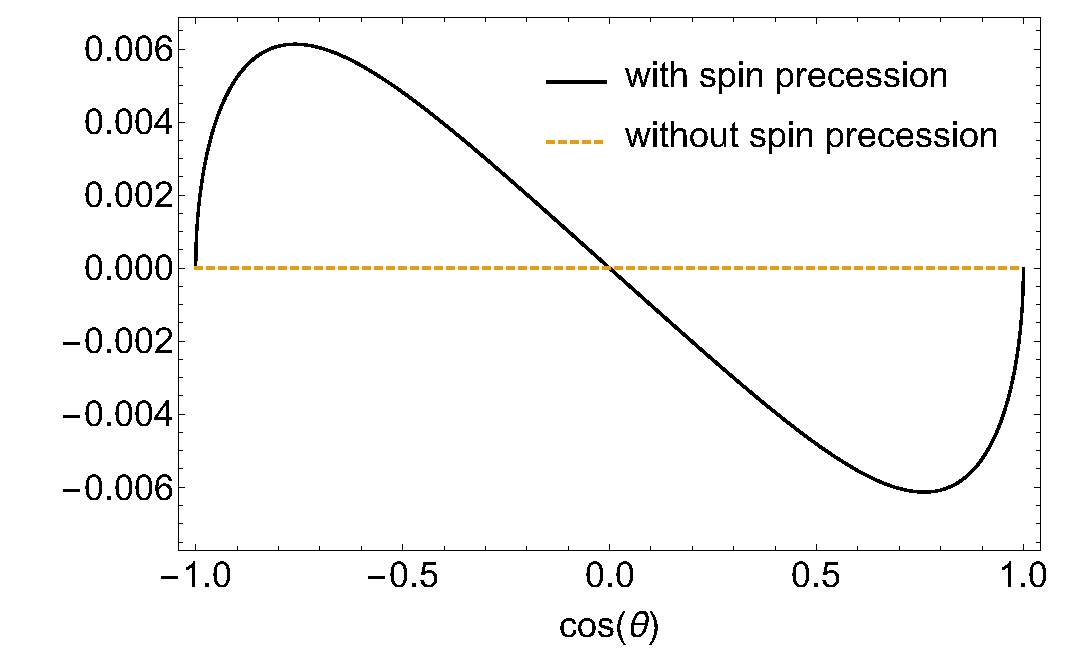
\includegraphics[width=0.9\linewidth]{figures/spin/px.eps}
    \caption{%
        $P_{\Lambda}^{y}$的分布。
    }%
    \label{fig:px}
\end{figure}
\section{蒙特卡洛模拟分析}
在实验上,自旋进动效应常常被忽略。在本节中,我们将利用蒙特卡洛模拟来研究忽略自旋进动效应带来的实验偏差。
参数$\alpha_{\psi}$, $\Phi$及$\alpha_{\pm}$的值的选择根据文献\cite{Ablikim:2018zay}的测量结果。
在模拟中不考虑任何$CP$破坏来源,假定$\alpha_{\pm}=\pm0.750$,同时
令$\alpha_{\psi}=0.462$, $\Phi=0.738$。探测器内部的磁场强度设为1T,对撞能点为$\sqrt{s} = $ 3.097 GeV, $\Lambda$
的动量为$\sqrt{s/4 - m^2}$。

蒙特卡洛产生子的基于ROOT\cite{ROOT}框架实现。在相空间事例的基础上,用形状\ref{eq:pdf}去随机舍取
一定的事例以得到蒙特卡洛样本。

为了揭示自旋进动效应对参数$\alpha_{\psi}$, $\Phi$ 和$\alpha_{\pm}$的影响,特别是对$CP$破坏测量的
影响, 对蒙特卡洛样本进行拟合以得到相应的参数值。几率密度函数的定义为
\begin{equation}
    \mathcal{P} = \frac{1}{N} \frac{{\rm d} \sigma}
    {{\rm d } \cos\theta {\rm d} \Omega_1 {\rm d} \Omega_2},
\end{equation}
式中$N$是归一化常数。经过积分得到其大小为$(4\pi){}^{2}(1 + \alpha_{\psi}/3)$。随后得到似然函数为:
\begin{equation}
    - \ln\mathcal{L} = -\sum_{i=1}^{n} \ln \mathcal{P}_{i},
\end{equation}
式中$i$代表蒙特卡洛样本中的第$i$个事例,$n$是样本的总事例数,其值为$1 \times 10^{6}$。
为了更好的区分,我们用脚标${}^{\rm truth}$表示基于修正后的形状\ref{eq:pdf}的拟合值,
而用脚标${}^{\rm biased}$表示基于未考虑自旋进动效应的形状的拟合值。
两组值之间的差异为:
\begin{equation}
    \begin{aligned}
        %\Delta \alpha &= \alpha^{\rm corr} - \alpha^{\rm exp}\\
        %\Delta \Phi  &= \Phi^{\rm corr} - \Phi^{\rm exp}\\
        \Delta \alpha_{\pm} & = \alpha_{\pm}^{\rm biased} - \alpha_{\pm}^{\rm truth} 
    \end{aligned}
\end{equation}

\begin{figure}[h!]
    \centering
    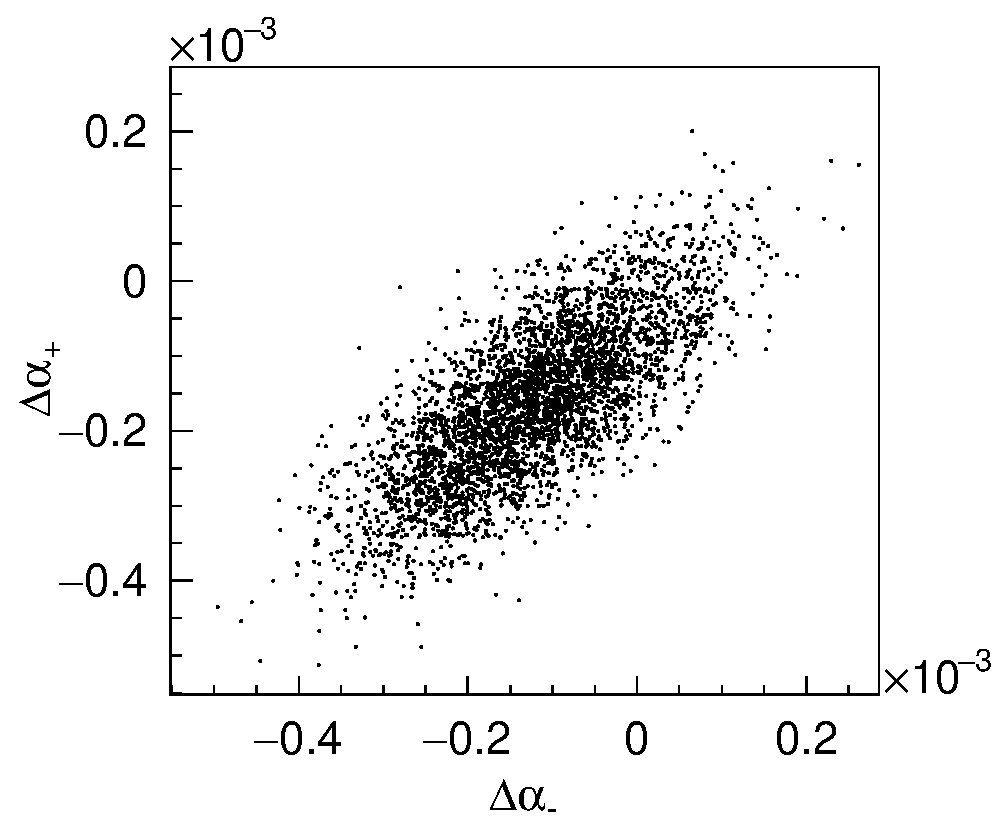
\includegraphics[width=0.8\linewidth]{figures/spin/corr.eps}
    \caption{%
        $\Delta \alpha_{-}$与$\Delta \alpha_{+}$之间的强关联。
 Each black point denotes the result from fitting to each toy MC sample.}%
    \label{fig:corr}
\end{figure}
我们产生了4000份蒙特卡洛样本,每个样本大小都相同,实验发现$\Delta \alpha_{-}$和$\Delta \alpha_{+}$之间有强烈的
关联,如图\ref{fig:corr}所示,图中的每个黑色的点均为一次实验的结果,点的疏密分布显示出很强的相关性。
这个强相关性将导致对$CP$破坏测量出现一定的偏差:
\begin{equation}
    \begin{split}
       \Delta A_{CP} &= \frac{1}{n}  \sum_{i=1}^{n} 
         \frac{\Delta \alpha_{-, i} + \Delta \alpha_{+, i}}
         {\alpha_{-, i}^{\rm biased} - \alpha_{+, i}^{\rm biased}} \\
        &=  (-1.9 \pm 0.1) \times 10^{-4}, 
    \end{split}
\end{equation}
式中$i$表示对第$i$个蒙特卡洛样本的结果, $n=4000$是实验的总次数。
这里使用了$CP$守恒条件,即$\alpha_{-}^{\rm truth} + \alpha_{+}^{\rm truth} =0$。
由此得到的$\Delta A_{CP}$大小是标准模型预言值的若干倍,正如图\ref{fig:acp}展示的。 
当增大磁场的强度时,如图\ref{fig:varyB}所示,和预期一致,$\Delta A_{CP}$的大小几乎线性地增加。
同时我们也观测到$\alpha_{\psi}$和$\Phi$也会分别偏离约0.07\% 和 0.01\%。
\begin{figure}[htpb]
    \centering
        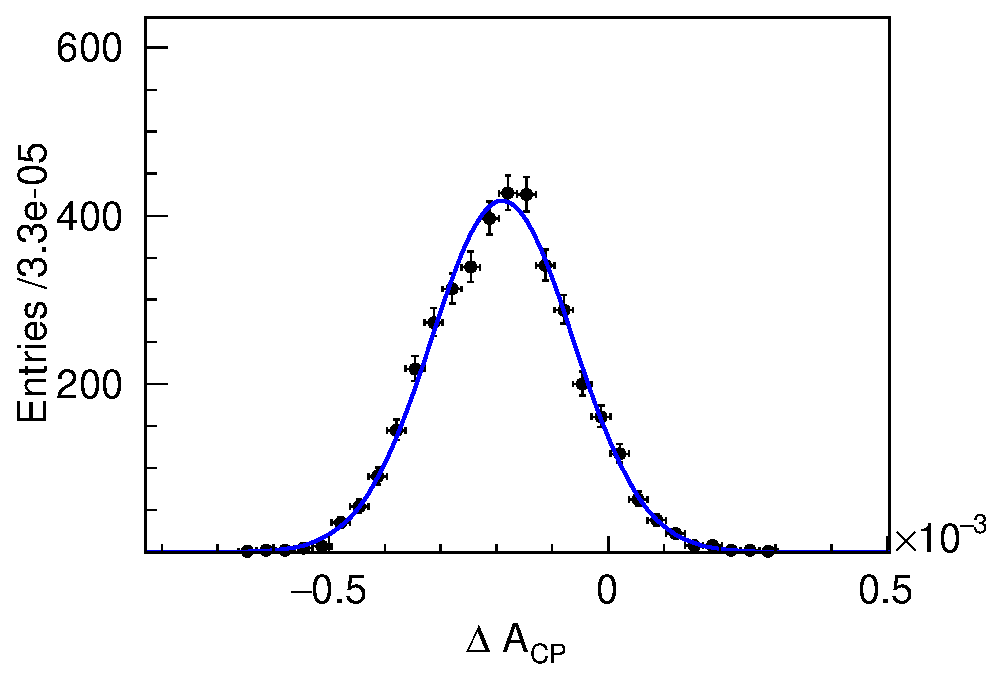
\includegraphics[width=0.9\linewidth]{figures/spin/afit.eps}
        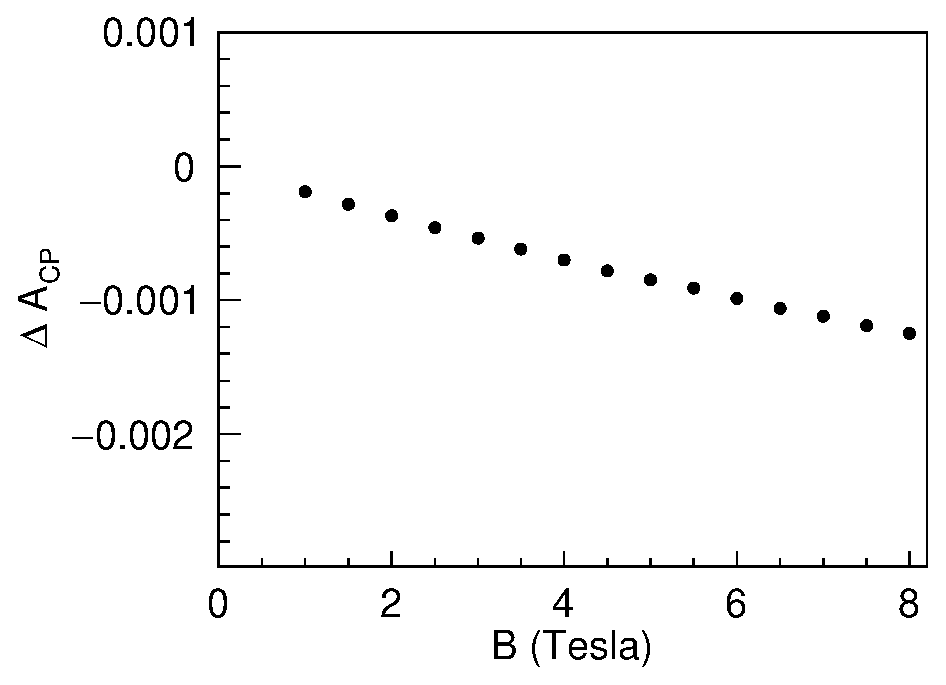
\includegraphics[width=0.9\linewidth]{figures/spin/Acp.eps}
    \caption{(a)$\Delta A_{CP}$的分布。 
    (b) 增大探测器内部的磁场的强度。}%
    \label{fig:acpandvaryB}
\end{figure}
\section{总结和讨论}
本章节考虑了磁场对超子对角分布的影响。由于超子存在磁矩,引起其自旋方向将会绕磁场转动,考虑
到这项修正,我们得到了整体的微分截面,微分截面的修正项与$\Lambda$的寿命成正比。
通过蒙特卡洛模拟,本节定量的考虑了磁场修正项的影响,并得到了一个重要的结论:一旦忽略磁场的影响,
实验上对 $CP$破坏的测量将不可避免的引入$10^{-4}$的偏差,这个偏差和标准模型预言的$CP$破坏大小相当。
于此同时,$\alpha_{\psi}$ 和 $\Phi$测量也会有微小的偏差,$\Lambda$的极化的观测也受到影响。

本文研究的这项效应,在其他的文献里\cite{Kharzeev:2015znc,Guo:2019joy,Deng:2018frf}也被研究了。
安装类似的方法,很容易把研究范围扩展到其他的超子对的产生,比如$\Xi\bar{\Xi}$, $\Sigma^{0}
\bar{\Sigma}^{0}$, $\Omega\bar{\Omega}$等。这个效应的影响比较小,目前的数据量有限不足以显示出
这项效应的影响, 但是在未来的超级粲陶工厂中,实验的灵敏度可达到$10^{-4}$甚至$10^{-5}$\cite{Bigi:2017eni},
这个效应的影响将起重要作用。 

\chapter{研究$J/\psi$的极化及其影响}%
\section{简介}
只有深刻的认识到$J/\psi$的状态才能更深一步的研究其衰变性质
。正负电子对产生的$J/\psi$
与正负质子对、质子对撞、$B_{s}$衰变、$\psi(2S)$衰变、$\chi_{cJ}$衰变的极化状态截然不同,
% https://arxiv.org/pdf/1909.03370.pdf B_{s} -> phi J/psi
其中最重要的差别是$J/psi$的极化状态不同。这一节是研究超子对产生性质的前奏。在下面的小
节中,将首先论述正负电子对产生的$J/\psi$的极化状态,接着以$J/\psi \to e^{+} e^{-} P$为例
说明极化状态对实验测量的影响,并对其分支比进行了预言。
\subsection{$\psi$的极化状态}
在这一章节中,我们将研究正负电子对撞机产生的$J/\psi$极化状态。一般的,有质量的矢量粒子有三种极化状态,它们分别是:
\begin{equation}
  \begin{split}
    \epsilon^{\mu}_{\rm{LP}} &= (0,0,0,1) \\ 
    \epsilon^{\mu}_{\rm{TL}} &= \frac{1}{\sqrt{2}}(0,1,-i,0) \\ 
    \epsilon^{\mu}_{\rm{TR}} &= \frac{1}{\sqrt{2}}(0,1,i,0)
  \end{split}
\end{equation}
式中的$\epsilon^{\mu}_{\rm{LP}}$,  $\epsilon^{\mu}_{\rm{TL}}$ 及 $\epsilon^{\mu}_{\rm{TR}}$分别
代表纵向极化,左旋及右旋极化状态。

考虑到洛伦茨不变性及宇称守恒过程$e^{+} e^{-} \to \psi$的振幅的一般形式为 
\begin{equation}
    T = e_{c} e f_{\psi} \frac{m_{\psi}}{q^{2}} 
    \bar{u}(k_{1}) \gamma_{\mu} \nu(k_{2}) \epsilon^{\mu}
\end{equation}
式中$e_{c}$和$e$分别是$c$夸克和电子电荷,$m_{\psi}$为$\psi$介子的质量,$k_{1}$ ($k_{2}$)是
电子(反电子)的动量,$\epsilon^{\mu}$是$\psi$的极化矢量。
很容易得到$|T|^{2}$为:
\begin{equation}
\begin{split}
|T(\psi)|^{2} =  & \frac{16\pi^{2}\alpha^{2}e^{2}_{c}}{q^{4}}|f_{\psi}|^{2}m^{2}_{\psi}\epsilon^{*}_{\mu}\epsilon_{\nu} \\ & \times (k^{\mu}_{1}k^{\nu}_{2} + k^{\mu}_{2}k^{\nu}_{1} - g^{\mu\nu}k_{1}\cdot k_{2} + g^{\mu\nu}m^{2}_{e}),
\end{split}
\end{equation}
式中的$m$为电子的质量,$q=k_{1}+k_{2}$。
经过简单的计算可以得到三种极化状态的相对比例为:
\begin{equation}
\begin{split}
|T( \psi)|^{2}_{\rm{LP}}:|T(\psi)|^{2}_{\rm{TL}}:|T( \psi)|^{2}_{\rm{TR}} = m^{2}_{e}:m^{2}_{\psi}:m^{2}_{\psi} 
  \approx 2.7 \times 10^{-8} :1 : 1 。
\end{split}
\end{equation}
这个计算结果表明纵向极化的大小和电子质量平方成正比,与文献\cite{Richman:1984gh}中的结论一致,
量级很小,可以忽略不记。同时可以推测$\mu^{+}\mu^{-}$
对撞产生的$J/\psi$的纵向极化将远大于$e^{+}e^{-}$产生的。
这个结论很容易扩展到$J/\psi$的激发态的产生,乃至于$\Upsilon$的产生情况。

\subsection{以$J/\psi \to e^+ e^- P$为例研究极化的影响}
$J/\psi \to e^+ e^- P$是一个电磁相互作用主导的达利兹衰变,这里的$P$代表一个
赝标量粒子。这个衰变道提供了一个理想的环境去研究强子的结构,特别是光子和强子之间
的相互作用\cite{Landsberg:1986sk, Landsberg:1986fd}。末态的轻子对来自于$J/\psi$ 跃迁到$P$
所辐射的离壳的光子,这个过程能够被QED理论精确的描述\cite{Kroll:1955zu},除了一个转移动量依赖的
形状因子$f_{\rm VP}(q^{2})$不得不借助于QCD模型\cite{Achasov:1992ku, Klingl:1996by, Faessler:1999de,
Terschluesen:2010ik, Ivashyn:2011hb}。需要指出的理论上已经对 $J/\psi$和$P$之间的跃迁做了广泛的
讨论\cite{Shifman:1979nx, Khodjamirian:1983gd, Beilin:1985da, Zhang:1991et, Ebert:2002pp, Lahde:2002wj, 
Hwang:2006cua,  Dudek:2006ej, Ke:2010pp, Donald:2012ga, Becirevic:2012dc,Pineda:2013lta}。但是,之前的研究侧重于
对衰变分支比的预言,故没有讨论初态粒子的极化。比如在文献\cite{Fu:2011yy}中,作者假设初态的$J/\psi$是完全没有极化的,
这简化了理论计算,但是实验家也对末态粒子的角分布感兴趣,一方面角分布之中包含了额外的信息,另一方面蒙特卡洛模拟的效率
强烈的依赖于粒子的角分布,这也是本章节的出发点之一。
 在实验上,许多$J/\psi$到$P$的跃迁过程以及被观测到了,我们把相关的测量总结在表\ref{tab:summaryresult}中,
比如实验上已经确定了
${\cal B}(J/\psi \to \gamma\eta_{\rm c}(1S)) = (1.7 \pm 0.4) \%$~\cite{Tanabashi:2018oca}。
 然而${\cal B}(J/\psi \to e^{+} e^{-} \eta_{\rm c}(1S))$尚待被
测量。
\begin{table}[!htbp]
    \centering
    \caption{%
        实验上已经观测到的$V \to P l^{+} l^{-}$的分支比及其与辐射衰变宽度的比值\cite{Tanabashi:2018oca}。
    }%
    \label{tab:summaryresult}
    \begin{tabular}{p{3.5cm}p{3.5cm}<{\centering}p{3.5cm}<{\centering}}
        \toprule
        衰变模式  &  分支比 &  $\frac{\Gamma(V \to P l^{+} l^{-})}{\Gamma(V \to P \gamma)}$  \\
        \midrule
        $\rho^{0} \to \pi^{0} e^{+}  e^{-}$  &  $<1.2 \times 10^{-5}$ &  $<2.6 \times 10^{-2}$   \\
        $\omega \to \pi^{0} e^{+}  e^{-}$  &  $(7.7\pm0.6) \times 10^{-4}$  &  $(0.91\pm0.08) \times 10^{-2}$    \\
        $\omega \to \pi^{0} \mu^{+}  \mu^{-}$  &  $(1.34\pm0.18) \times 10^{-4}$  &  $(0.16\pm0.02) \times 10^{-2}$     \\
        $\phi \to \pi^{0} e^{+}  e^{-}$  &  $(1.33^{+0.07}_{-0.10}) \times 10^{-5}$  &  $(1.02^{+0.07}_{-0.09}) \times 10^{-2}$    \\
        $\phi \to \eta e^{+}  e^{-}$  &  $(1.08\pm0.04) \times 10^{-4}$  &  $(0.83\pm0.03) \times 10^{-2}$    \\
        $\phi \to \eta \mu^{+}  \mu^{-}$  &  $<9.4 \times 10^{-6}$  &  $<0.07 \times 10^{-2}$    \\
        $J/\psi \to \pi^{0} e^{+} e^{-}$  &  $(7.6\pm1.4) \times 10^{-7}$   & $(2.18^{+0.45}_{-0.44}) \times 10^{-2}$  \\
        $J/\psi \to \eta e^{+} e^{-}$  &  $(1.16\pm0.09) \times 10^{-5}$  &  $(1.05\pm0.09) \times 10^{-2}$  \\
        $J/\psi \to \eta^{\prime} e^{+} e^{-}$  &  $(5.81\pm0.35) \times 10^{-5}$  &  $(1.13\pm0.08) \times 10^{-2}$   \\
        $\psi^{\prime} \to \eta^{\prime} e^{+} e^{-}$  &  $(1.90\pm0.27) \times 10^{-6}$   &  $(1.53\pm0.22) \times 10^{-2}$   \\
        \bottomrule
    \end{tabular}%
\end{table}
用如下的比值能够较好的预测$\psi \to e^+ e^-  \eta_c$的分支比
\begin{equation}
\label{eq:R-jpsipolar}
    R \equiv \frac{B(\psi \to e^+ e^-  \eta_c)}{B(\psi \to \gamma \eta_{c})},
\end{equation}
一个突出的优势是很多理论的不确定性相互抵消。
一般的,$V \to P e^{+} e^{-}$的衰变振幅为\cite{Landsberg:1986sk,Landsberg:1986fd,Fu:2011yy}
\begin{equation}
T(V \to P l^{+}l^{-}) = 4 \pi \alpha f_{V\!P}\epsilon^{\mu\nu\rho\sigma}p_{\mu}q_{\nu}\epsilon_{\rho}\frac{1}{q^{2}}\bar{u}_{1} \gamma_{\sigma} \nu_{2},
\end{equation}
式中的$\alpha$为精细结构常数,$f_{V\!P}$是跃迁形状因子,$\epsilon^{\mu\nu\rho\sigma}$是列维-西塔张量,
$p_{\mu}$是赝标量粒子的动量,$q_{\nu} = k_{1}+k_{2}$ 其中$k_{1}$和$k_{2}$分别是轻子$l^{+}$和$l^{-}$的动量。
仅对末态的轻子的自旋求和可得到
\begin{equation}
    |T(V \to P l^{+} l^{-})|^{2} = 16\pi^{2}\alpha^{2}\frac{|f_{V\!P}(q^{2})|^{2}}{q^{4}} \cdot h ,
\end{equation}
这里的
\begin{equation}
\begin{split}
    h &=  8 m^{2}_{V} m^{2}_{l} (q^{2} \epsilon \cdot \epsilon^{*} - q \cdot \epsilon  q \cdot \epsilon^{*} ) \\
       & -2 m^{2}_{V} q^{4}(k_{1} - k_{2} )\cdot \epsilon (k_{1}  - k_{2}) \cdot \epsilon^{*}
      \\ & +8m^{2}_{l} q\cdot p
        [q \cdot \epsilon  p.\epsilon^{*} - \epsilon \cdot \epsilon^{*} q \cdot p]
      \\ & +2m^{2}_{l}(k_{1} - k_{2} )\cdot p
      \\ & \times [\epsilon \cdot \epsilon^{*}(k_{1} - k_{2} )\cdot p + (k_{1}  - k_{2} ) \cdot \epsilon (p\cdot\epsilon^{*})]
      \\ & +8 [(k_{2} \cdot p)(k_{1}\cdot \epsilon)  - (k_{1} \cdot p)(k_{2} \cdot \epsilon)]
      \\ & \times [(k_{2} \cdot p)(k_{1}\cdot \epsilon^{*})  - (k_{1} \cdot p)(k_{2} \cdot \epsilon^{*})] ,
\end{split}
\end{equation}
式中的$m_V$和$m_l$分别是矢量和赝标量粒子的质量,相应的衰变微分宽度为
\begin{equation}
\label{eq:width-PVLL}
\begin{split}
    d\Gamma(V\to Pl^{+}l^{-})=~& \frac{1}{(2\pi){}^{5}} \frac{1}{16m_{V}^{2}} |T(\psi(\Upsilon) \to P l^{+} l^{-})|^{2} \\ & \times {\bf |k^{*}|}{\bf |p_{3}|} dm_{l^{+}l^{-}} d\Omega_{3}d\Omega^{*}_{1},
\end{split}
\end{equation}
式中的$\bf |k^{*}|$的$l^{+}$或者$l^{-}$在$l^{+} l^{-}$对的质心系下的动量,
$d\Omega^{*}_{1} = d \phi^{*}_{1}d(\cos\theta^{*}_{1})$是其相应的立体角微分元,
$\bf |p_{3}|$是末态赝标量粒子在初态矢量粒子
质心系下的动量,$d\Omega_{3} = d \phi_{3}d(\cos\theta_{3})$代表其相应的立体角微分元。
\begin{figure}[!htbp]
\centering
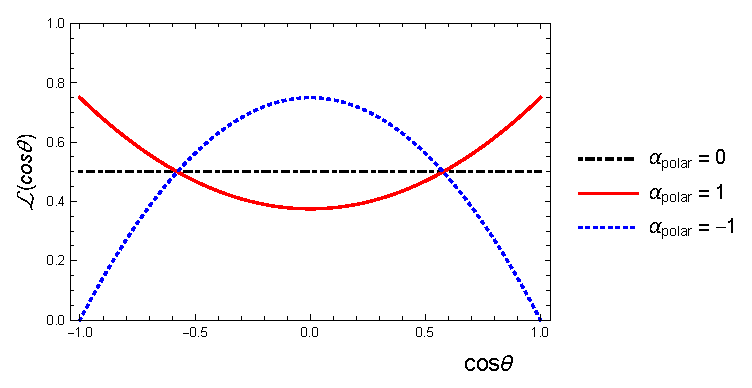
\includegraphics[width=0.9 \linewidth]{figures/angle.eps}
\caption{%
    末态赝标量粒子的极角的分布。
     黑色的虚线表示初态无极化的情况,红色的实线和蓝色的虚线分别代表只有横向极化和纵向极化的情形。
    }%
\label{fig:angle}
\end{figure}
实验家们感兴趣的是末态赝标量(或正负电子对)飞行方向的分布,我们把初态$J/\psi$的三种极化状态分布代入
公式\ref{eq:width-PVLL}之中可以得到:
\begin{equation}
\begin{split}
    & \frac{d\Gamma(\psi(\Upsilon) \to Pl^{+}l^{-}){}_{\rm{LP}}}{d\cos\theta} \sim  1- \cos^{2}\theta
    \\ & \frac{d\Gamma(\psi(\Upsilon) \to Pl^{+}l^{-}){}_{\rm{TL}}}{d\cos\theta} \sim \frac{1+ \cos^{2}\theta}{2}
    \\ & \frac{d\Gamma(\psi(\Upsilon) \to Pl^{+}l^{-}){}_{\rm{TR}}}{d\cos\theta} \sim \frac{1+ \cos^{2}\theta}{2},
\end{split}
\label{equ:angle}
\end{equation}
这里$\theta=\theta_3$即是$P$粒子在$J\psi$质心系下的极角。从而,我们可以借助于末态赝标粒子的方向信息
确定初态矢量粒子的极化状态。比如用如下的几率密度函数做拟合
\begin{equation}
     \mathcal{P}(\cos\theta) = 1 + \alpha_{\rm{polar}} \cos^{2}\theta,
\end{equation}
式中的$\alpha_{\rm polar}$用来衡量极化的大小。当$\alpha_{\rm polar} = +1$时,初态只有横向极化,
当$\alpha_{\rm{polar}} = -1$时,初态则只有纵向极化。图\ref{fig:angle}中展示了几种可能的极化状态。

\subsection{估算$\psi \to \eta_c l^{+} l^{-}$的分宽度}
从表\ref{tab:summaryresult}中列举的结果来看,衰变过程$\psi \to \eta_c l^{+} l^{-}$尚为被发现,
本小节利用公式\ref{eq:R-jpsipolar},即$\Gamma(\psi \to \eta_{c} l^{+} l^{-})$与$\Gamma(\psi \to \eta_{c} \gamma)$
的比值,来估算$\psi \to \eta_c l^{+} l^{-}$的分宽度。
过程$\psi(\Upsilon) \to P \gamma$的分宽度公式已经有文献\cite{Fu:2011yy}做了讨论,
我们直接引用其公式:
\begin{equation}
\frac{d\Gamma(\psi(\Upsilon)\to Pl^{+}l^{-})}{dq^{2}\Gamma(\psi(\Upsilon) \to P \gamma)} 
    = |F_{V\!P}(q^{2})|^{2} \times [{\rm QED}(q^{2})],
\label{equ:calVPll}
\end{equation}
式中用了正则化的形状因子$F_{V\!P}(q^{2}) \equiv
f_{V\!P}(q^{2})/f_{V\!P}(0)$,${\rm QED}(q^{2})$代表点粒子
假设下的微分宽度,即
\begin{equation}
\begin{split}
    {\rm QED}(q^{2}) = & \frac{\alpha}{3\pi} \frac{1}{q^{2}}
    \left(1-\frac{4m^{2}_{l}}{q^{2}} \right ){}^{\frac{1}{2}} \left(1 +
    \frac{2m^{2}_{l}}{q^{2}} \right)  \\ & \times \left[ \left(1 +
    \frac{q^{2}}{m^{2}_{V} - m^{2}_{P}} \right){}^{2}  -
    \frac{4m^{2}_{V}q^{2}}{(m^{2}_{V} - m^{2}_{P}){}^{2}} \right]
    {}^{\frac{3}{2}}.
\end{split}
\end{equation}
在实验上,只需要测量轻子对的能谱并与点粒子假设的理论结果做对比就能得到跃迁形状因子\cite{Landsberg:1986fd}。
由于缺少必要的实验数据,这里采取被广泛接受的VDM(vector dominance model)模型\cite{GellMann:1961tg, Bauer:1977iq},
因此在单极点近似下跃迁形状因子的形式为:
\begin{equation}
\label{fractor}
F_{V\!P}(q^{2}) = \frac{1}{1-\frac{q^{2}}{\Lambda^{2}}},
\end{equation}
这里的$\Lambda$表示一个矢量传播子的质量。
在过程$\psi \to \eta_{c} l^{+} l^{-}$中,极点的质量选取为$\psi^{\prime}$或$\psi(3770)$的质量。
我们变动极点的位置以研究衰变宽度对$\Lambda$依赖。数值计算结果表明衰变宽度对极点$\Lambda$的取值
不敏感,这很显然,因为$\Lambda$的取值远大于$q^{2}$。故我们选择$\Lambda =m_{\psi^{\prime}}$,
来计算相关的衰变宽度, 计算结果见表\ref{tab:VPll}。Fig.\ref{fig:parW}.
\begin{figure}[!htbp]
\centering
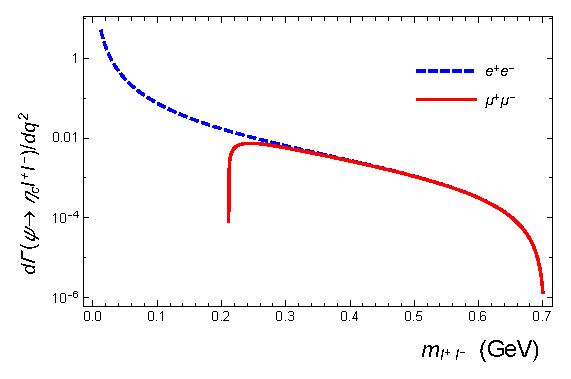
\includegraphics[width=0.9 \linewidth]{figures/partialW.eps}
\caption{过程$\psi^{\prime} \to \eta_c l^{+} l^{-}$的微分宽度。红线和蓝线分别代表$\psi^{\prime} \to \mu^+ \mu^-$
和$\psi^{\prime} \to \eta_c e^+ e^-$。}%
\label{fig:parW}
\end{figure}

\begin{table}[!htbp]
  \centering
  \caption{估计过程$\psi \to \eta_{c} l^{+} l^{-}$的分宽度。计算采取VDM模型,
    并取$\Lambda = m_{\psi^{\prime}}, m_{\psi(3770)}$ 。
    其中的误差来自于实验上$\Gamma(\psi \to \eta_{c} \gamma)$的测量结果。}%
  \label{tab:VPll}
  \begin{tabular}{p{3.5cm}p{2.5cm}<{\centering}p{2.5cm}<{\centering}}
  \toprule
   过程  &  $\Gamma^{VDM}_{ e^{+}e^{-}}$ (keV)  &  $\Gamma^{VDM}_{ \mu^{+}\mu^{-}}$ (keV) \\
  \midrule
   $J/\psi  \to \eta_{c} l^{+}  l^{-}$  &  $(9.6 \pm 2.3) \times 10^{-3}$   &  -\\
   $\psi^{\prime}  \to \eta_{c} l^{+}  l^{-}$   &  $(8.9 \pm 1.3)  \times 10^{-3}$  &  $(8.2\pm1.2) \times 10^{-4} $    \\
   %$\Upsilon({\rm{2S}}) \to \eta_{b} l^{+} l^{-}$   &  $(10.8 \pm 4.2) \times 10^{-5}$  &  $(8.2 \pm 3.2) \times 10^{-6}$    \\
   %$\Upsilon({\rm{3S}}) \to \eta_{b} l^{+} l^{-}$   &  $(9.7\pm1.6) \times 10^{-5}$  &  $(12.6\pm2.1) \times 10^{-6}$    \\
  \bottomrule
  \end{tabular}
\end{table}

\section{总结和讨论}
我们讨论了正负电子对撞机产生的$J/\psi$的极化状态,发现横向极化占主导地位,比纵向极化的强度
高出大约8个数量级。在这个结论的基础了,我们探讨了$J/\psi \to e^{+} e^{-} P$的衰变,发现极化对末态赝标量的极角影响较大,
其分布的$1+\alpha \cos^{2} \theta$,其中的$\alpha$与初态$J/\psi$的极化紧密相关,这对研究$J/\psi$极化状态
有重要的意义。同时我们预测了实验上为观测到的$\psi \to \eta_{c} e^{+} e^{-}$的宽度。
至今北京谱仪已经采集到了$10^{10}~J/\psi$和$4\times 10^{8}~\psi(2S)$样本,如果采取部分重建方法,
只重建正反电子对,并假设典型的实验效率为10\%,我们预计将分别观测到
$10^{5}$和$10^{3}$个信号。这能够精确测量分支比,甚至测量跃迁形状因子。

% ====================================================
%   Copyright (C)2019 All rights reserved.
%
%   Author        : Xin-Xin Ma
%   Email         : xxmawhu@163.com
%   File Name     : jpsi_sigma0.tex
%   Last Modified : 2019-12-11 19:07
%   Describe      :
%
% ====================================================%
\chapter{在$J/\psi$和$\psi(2S)$上研究超子$\Sigma^{0}$的极化及寻找CP破坏}%
\label{cha:polarization}
\section{简介}%
\label{sec:Sigma0-introduction}
自从质子的内部结构被首次发现以来,研究重子的内部结构始终是个活跃的领域。
重子和电磁场的相互作用项包含两项,电形状因子和磁形状因子。电子束流是探测
重子内部结构的有力探针。然而为了研究定量的研究电磁形状因子,需要用极化的
电子束流,实验的难度很大,一直到1976年SLAC实验室首次公布的极化的电子束流打
靶的实验结果\cite{Alguard:1976bk},在这个实验中电子束流和质子靶都是极化的。
然而,这个实验方案对于超子而言完全不可行,因为超子的寿命都极短,
约为$10^{-12}s$。

正负电子对撞是研究超子电磁形状因子的理想平台,其中重要的原因是电子对能够产生
在部分方向上极化的超子,能够有效的探测到超子的电磁形状因子。在2018年BESIII
合作组发现了在$J/\psi \to \Lambda \bar{\Lambda}$过程中的$\Lambda$是部分
极化的。对超子的进一步理解需要更多的测量,因此对重子八重态的一系列研究
仍十分迫切,本文选择超子$\Sigma^{0}$作为研究对象。$J/\psi$和$\psi(2S)$提供了
大量的$\Sigma^{0}\bar{\Sigma}^{0}$对作为研究的样本。

与$\Lambda$超子略微不同的是,$\Sigma^{0}$是电磁衰变主导,应当遵循
严格的P宇称守恒。如果发现弱相互作用的贡献,则可能观测到P宇称的破坏。
同时,中子的电偶极矩也会导致$\Sigma^{0}$衰变过程中的P宇称
破坏\cite{NAIR2019535}。
这些P宇称破坏项将导致一个非0的衰变参数$\alpha_{\gamma}$,这个衰变参数能够
检验$CP$守恒,因为$CP$守恒要求
\begin{equation}
    \alpha_{\gamma} = - \bar{\alpha}_{\gamma},
\end{equation}
式中$\bar{\alpha}_{\gamma}$是$\bar{\Sigma}^{0}$的相应的衰变参数。

\section{事例挑选}%
\label{sec:sigma-event-selection}
\subsection{带电径迹}%
\label{sec:sigma-good-track}
和小节\ref{sec:charged-track}类似,略微不同的是由于$\Lambda$飞行时间较长,
在探测器内部的平均飞行距离约10$cm$,因此带电径迹不是来自对撞点。本节
对带电径迹的要求稍变为
\begin{itemize}
    \item $z$方向上带电径迹与$e^{+}e^{-}$对撞顶点的投影距离满足:
        $R_{z} < 10 cm$;
    \item 带电径迹的初始动量方向的极角满足:$|\cos\theta| < 0.93$。
\end{itemize}

\subsubsection{粒子鉴别}
在实验上通常需要对带电径迹做粒子鉴别从而准确的重建信号并压低本底,
一个缺点是粒子鉴别程序总会不可避免的带来系统误差,有时候还是主导
的系统误差。本文通过研究发现仅仅用运动学信息就能足够把质子和$\pi^{+}$
介子区分开,能降低系统误差,并同时稍微提高效率。
图\ref{fig:momenta-of-pr-pion}展示了质子和$\pi^{+}$介子的动量分布, 可以明显的
看出两者的动量明显不同,由于质子质量较大,携带了大量的动量,其动量大小从而
都在450 MeV$/c$以上,与之相反,$\pi^{+}$介子的动量都在450 MeV$/c$一下,因此本文选择
用动量大小作为粒子鉴别的重要手段,动量小于$450$~MeV$/c$的带电径迹作为$\pi^{+}$
候选者,大于450 MeV$/c$的视为质子。
% /besfs/groups/jpsi/jpsigroup/user/maxx/Jpsi/SS/664/noDangCut/signal/draw/fig/
\begin{figure}[htbp]
    \centering
    \mbox{%
        \begin{overpic}[width = 0.5\linewidth]{jpsi/eventsele/pPrandPi.eps}
            \put(38, 58) {\color{gongnvlan} $(MC)$}
        \end{overpic}
        \begin{overpic}[width = 0.5\linewidth]{jpsi/eventsele/pPrandPiBar.eps}
            \put(38, 58) {\color{gongnvlan} $(MC)$}
        \end{overpic}
    }
    \caption{%
        信号蒙特卡洛样本中的质子和$\pi$介子的动量分布图。红色的直方图表示正反质子
        的动量分布,蓝色的是$\pi^{\pm}$的动量分布。红色的箭头表示粒子鉴别
        的要求。
    }%
    \label{fig:momenta-of-pr-pion}
\end{figure}

\subsection{中性径迹}%
\label{sec:sigma-neutral-track}
除了带电粒子,末态中还包含中性的粒子,种类只有一种,就是孤立的光子。
孤立光子的选择条件和小节\ref{sec:ds-neutral-track}完全一样,因此不再详细叙述。

\subsection{$\Lambda$重建}
$\Lambda$在探测器内飞行较短的路程后衰变为一对带电粒子从而得以被重建。
这对带电径迹的顶点偏离对撞点,为了提高$\Lambda$的质量分辨率需要对其做
次级顶点拟合。本文要求次级顶点拟合的$\chi^{2}$小于100,经过顶点拟合之后
的$\Lambda$的质量需要落在区间[1.110, 1.120] GeV$/c^{2}$内。

\subsection{运动学拟合}
运动学拟合能够提高粒子重建动量的分辨率。本文对末态粒子$\Lambda$,
$\bar{\Lambda}$,$\gamma_{1}$,$\gamma_{2}$进行运动学拟合(其中$_{1,2}$
仅仅是对光子的编号),一方面为了提高重建动量的分辨率,另一方面由于本底难以
通过运动学拟合,因此利用运动学拟合能够筛选信号、压低本底。在运动学拟合中,
我们要求末态粒子的总能量与对撞能量相等,动量等于正负电子束流的总动量,这里
共有四个约束条件,因此称之为4C运动学拟合。如果单个事例中
有多个组合能通过上述的筛选条件,本文只保留4C运动学拟合$\chi^{2}$最小的组合
作为唯一的候选者。4C运动学拟合的$\chi^{2}$分布图见\ref{fig:cut-chisq-sigma0},
我们从信噪比和系统误差两方面综合考虑来决定对$\chi^{2}$的要求条件。
一方面从图\ref{fig:cut-chisq-sigma0}可以看出提高$\chi^{2}$的截断值到100以上
时信噪比的增加微乎其微,但是本底水平会略增,当对$\chi^{2}$的截断较小时,
从图\ref{fig:diff}可以看出系统误差会明显增大,故要求$\chi^{2}$小于100。
% /besfs/groups/jpsi/jpsigroup/user/maxx/Jpsi/SS/664/noDangCut/inclusiveMC/chisq_cut/fig/
\begin{figure}[htbp]
    \centering
    \begin{overpic}[width = 0.45 \linewidth]{jpsi/eventsele/chisq.eps}
        \put(65, 40){(a)}
    \end{overpic}
    \begin{overpic}[width = 0.45 \linewidth]{jpsi/eventsele/Q.eps}
        \put(65, 40){(b)}
    \end{overpic}
    \caption{%
        (a) 4C运动学拟合的$\chi^{2}$。蓝色的实线为蒙特卡洛样本中的$\chi^{2}$分布,
        红线展示了本底水平及分布。
        (b) 不同的截断值对于的信噪比水平。红色的线表示本文所选择的截断值。
    }%
    \label{fig:cut-chisq-sigma0}
\end{figure}
% /besfs/groups/jpsi/jpsigroup/user/maxx/Jpsi/SS/664/noDangCut/Uncertainty/4C/controlSam/4cCut/
\begin{figure}[htbp]
    \centering
    \mbox{%
        \begin{overpic}[width = 0.8 \linewidth]{jpsi/eventsele/diff.eps}
        \put(25,70) {}
        \end{overpic}
    }
    \caption{%
        对4C运动学拟合的要求带来的系统误差。这项研究基于控制样本
        $J/\psi \to p\bar{p} \pi^{+}\pi^{-} \pi^{0}$。
        纵坐标为数据和蒙特卡洛样本之间的效率的 差异,误差棒代表数据中效率的统计误差。
        相关细节见:\ref{sec:KF}。
    }%
    \label{fig:diff}
\end{figure}


\subsection{$\Sigma^{0} (\bar{\Sigma}^{0})$候选者的挑选}
$\Sigma^{0}$主要是衰变模式为$\Sigma^{0} \to \Lambda \gamma$,分支比约为
99\%。$\Sigma^{0}$的重建方式是挑选一对合适的$\Lambda$和$\gamma$。
由于末态中含有两个光子,故存在两种组合:$\Lambda \gamma_{1}$,$\Lambda
\gamma_{2}$。为了挑选最佳的组合,本文对它们分别做运动学拟合,包含6个约束
条件,分别将总能量和总动量约束到$e^{+}e^{-}$的总能量和动量,此外将$\Lambda
\gamma$和$\bar{\Lambda} \gamma$的不变质量约束到$\Sigma^{0}$质量的世界平均
测量值~\cite{PDG}。在每个事例中,只有6C运动学拟合的$\chi^{2}$最小的一种组合
被保留做进一步的分析。6C拟合的另外一个好处是能够提高事例重建的动量分辨率,
有利于进一步对角分布的研究以抽取$J/\psi$及$\Sigma^{0}$的衰变参数。
在下文的研究中,对本底的分析将利于4C运动学拟合得到的末态动量信息,对其余
各项的研究则基于6C运动学拟合得到的末态动量信息。
\section{信号产额}
\subsection{本底分析}%
\label{sec:sigma-signal-yield}
本文根据衰变末态的不同将本底分成四类,这四类分别是
\begin{itemize}
    \item $\gamma \Lambda \bar{\Lambda}$ \\
        重建的末态中有一个$\gamma$是假光子,可能来自
        \textbf{EMC}中的噪音或者带电粒子和探测器的相互作用。
        通常,能产生这样的末态的来源有两个,其一是$J/\psi \to
        \Sigma^{0} \bar{\Lambda} + c.c$,但是这个衰变过程破坏同位旋
        守恒导致分宽度极小,从而可以忽略不计。另外一个是
        $J/\psi \to \gamma \eta_{c}, \eta_{c} \to \Lambda \bar{\Lambda}$,
        由于这个过程的相空间比较小,导致$J/\psi \to \gamma \eta_{c}$的
        分宽度比较小,因此这个过程贡献本底也很低。
    \item $\gamma \gamma \Lambda \bar{\Lambda}$\\
        这个过程的特点是和信号道的末态完全相同,区别在于至少有一对
        $\gamma \Lambda$($\bar{\Lambda}$)不是$\Sigma^{0}$
        ($\bar{\Sigma}^{0}$)衰变来的。典型的过程为$J/\psi \to \gamma
        \bar{\Lambda} \Sigma^{0} + c.c$,考虑到单纯的三体过程分宽度较低,
        因为辐射过程是压低的,更有可能是两体的过程。若其中的孤立光子来自超
        子的辐射,然而众多超子里面,只有$\Sigma^{0}\to \gamma \Lambda$分支比
        最大,其余的分支比都极低,因此这种过程的贡献也极低。另一种可能的过程
        是$J/\psi \to \gamma \eta_{c}, \eta_{c} \to \bar{\Lambda}
        \Sigma^{0} + c.c$,同样的由于同位旋的破坏而压低,因此可以忽略
        这种本底来源。综上所述,本文预期这个本底来源的贡献是可以忽略的。

    \item $\gamma \Sigma^{0} \bar{\Sigma}^{0}$ ($3\gamma \Lambda
        \bar{\Lambda}$)\\
        这个本底的特点是有个多余的光子,但是光子能量可能太低而不能被丢失,
        从而构成峰本底。考虑到这个光子最大的来源是$\Sigma^{0}$激发态的辐射
        衰变。然而这种过程的分支比都很低,比如${\Sigma(1385)}^{0} 
        \to \gamma \Sigma^{0}$,分支比约为$10^{-4} \sim 10^{-5}$,故这个本底
        的贡献也可以忽略不记。
    \item non-$\Lambda$ background \\
        这个本底的特点是末态完全没有$\Lambda$($\bar{\Lambda}$)超子,但是
        数据量大,带来的误组合本底可能比较显著。这种本底会在下文详细叙述,
        基于inclusive 蒙特卡洛样本的研究表明这种本底的贡献不高,约为0.2\%。
\end{itemize}
本底的定量估计所依赖的遍举过程的分支比取世界测量平均值~\cite{PDG},最主要的几项本底过程
见表~\ref{tab:background}。
\begin{table}[htbp]
    \caption{%
        几种主要的本底。基于蒙特卡洛研究每个本底预期的事例数,每个过程的分支比
        采取世界测量平均值~\cite{PDG}。
    }%
    \label{tab:background}
    \begin{center}
        \begin{tabular} {p{0.6 \linewidth} p{0.2\linewidth}}
            \toprule 
            本底过程  &  预期事例数 \\
            \midrule 
            $J/\psi \to \Lambda \bar{\Sigma}^{*0} +{\rm c.c}$ & $<112$ \\
            $J/\psi \to \Lambda \bar{\Sigma}^{0} + {\rm c.c}$ & 54\\
            $J/\psi \to \gamma \eta_c, \eta_c \to \Lambda \bar{\Lambda}
            $ & 42\\
            $J/\psi \to p \bar{p} \eta, \eta \to \pi^{+} \pi^{-}
            \pi^{0}$ & 17\\

            $J/\psi \to p \bar{p} \pi^{+} \pi^{-} \pi^{0}$ & 13 \\
            $J/\psi \to \Lambda \Lambda \pi^{0}$ & 10 \\
            $J/\psi \to \Sigma^{-} \bar{\Sigma}^{*+} + {\rm c.c}$ & 6 \\

            $J/\psi \to \gamma \eta_c, \eta_c \to \Lambda
            \bar{\Sigma}^{0} + {\rm c.c}$ &  Unknown \\

            $J/\psi \to \gamma  \Lambda
            \bar{\Sigma}^{0} + {\rm c.c}$ &  Unknown \\

            \bottomrule
        \end{tabular}
    \end{center}
\end{table}

\subsection{信号产额}
上文定性的分析了本底情况,预期本底水平很低。由于
$\Sigma^{0}\bar{\Sigma}^{0}$是成对产生的,因此本文采取如下策略来获取
信号数及本底数。首先将$M(\Sigma^{0})$的分布分为信号区和边带区见图~\ref{fig:signal-and-sideband},
然后再信号区和边带区分别拟合$\bar{\Sigma}^{0}$的不变质量谱以获取信号数及本底数。
\subsubsection{信号区和边带区}
为了确定信号区和边带区,本文首先对$\Sigma^{0}$质量谱做了极大似然法拟合。信号形状是三个高斯分布的
和,本底形状则是2阶的切比雪夫多项式。拟合的结果如图~\ref{fig:signal-and-sideband}所示。
信号中心值左右$3\sigma$的区域是信号区,信号区左右各选择一段区域作为
边带区如图~\ref{fig:signal-and-sideband}中的绿色箭头标识。

\begin{figure}[htbp]
    \centering
    \mbox{%
        \begin{overpic}[width = 0.5\linewidth]{jpsi/yield/mS0.eps}
        \put(25,70) {}
        \end{overpic}
    }
    \caption{%
        $\Sigma^{0}$的不变质量谱。两个红色箭头之间的区域表示信号区。
         信号区左右分别是两个边带区,各自用两个绿色箭头表示。
    }%
    \label{fig:signal-and-sideband}
\end{figure}

\subsubsection{信号产额}%
\label{sec:sigma-signal-yield}
为了确定信号数及本底数,本文安照类似的方法对上文所述的信号区和边带区内的事例
的$\bar{\Sigma}^{0}$的质量谱分别
做了极大似然法拟合。 类似的,信号形状依旧是三个高斯分布的和,本底是2阶切比雪夫
多项式,峰值本底用相应的蒙特卡洛样本中的形状来描述,这种峰本底是数目作为自由参数由拟合结果决定。
相应的拟合结果见图~\ref{fig:signal-region}。
从拟合结果可以看出总的$\bar{\Sigma}^{0}$个数为$115664 \pm352$,
这里将峰本底分为两种,前者同时在$\Sigma^{0}$和$\bar{\Sigma}^{0}$的不变质量谱上形成峰,
比如$J/\psi \to \gamma \Sigma^{0} \bar{\Sigma}^{0}$,后者只在$\bar{\Sigma}^{0}$的质量谱
上形成峰,在$M(\Sigma^{0})$的分布上则是平坦的,这种本底的数目拟合边带事例的$\bar{\Sigma}^{0}$来得到这种本底数目。
 拟合的结果见~\ref{fig:peak}。相应的比例因子是 ($\frac{S_{\rm
signal}}{S_{\rm side band}}$) 是1.69, 式中的 $S_{\rm signal}$ 和$S_{\rm
sidebade}$分布是本底分布在信号区和边带区内的积分,从而可以得到
这种峰本底的数目为$652
\pm 39$。 至此可以做个小结,通过前文的事例挑选过程,已经获取了纯度高达99.1\% 的样本以进行后续的研究,
相关的信号产额和本底见表~\ref{tab:yield}
\begin{figure}[htbp]
    \centering
    \mbox{%
        \begin{overpic}[width = 0.5\linewidth]{jpsi/yield/mS0bar.eps}
        \put(25,70) {}
        \end{overpic}
        \begin{overpic}[width = 0.5\linewidth]{jpsi/yield/mS0barLog.eps}
        \put(25,70) {}
        \end{overpic}
    }
    \caption{%
        $M(\gamma \bar{\Lambda}^{0})$的分布。两个红色箭头直接的区域代表信号区。
    }%
    \label{fig:signal-region}
\end{figure}

% /besfs/groups/jpsi/jpsigroup/user/maxx/Jpsi/SS/664/noDangCut/data/3
\begin{figure}[htbp]
    \begin{center}
    \mbox{%
        \begin{overpic}[width = 0.5\linewidth]{jpsi/yield/mpeak.eps}
        \put(25,70) {}
        \end{overpic}
    }
    \end{center}
    \caption{%
        对边带区的$\gamma\Lambda$不变质量谱的拟合结果。
        黑色的带误差棒的点代表数据。红色的点虚线代表信号形状,橙色的虚线展示了峰本底的形状,来源的
        $\Lambda$和一个假的低能的光子的组合。蓝色的实线是总的拟合结果。
    }%
    \label{fig:peak}
\end{figure}

\begin{table}[htbp]
    \caption{信号产额和本底数。}%
    \label{tab:yield}
    \begin{center}
        \begin{tabular} {p{0.4\linewidth} p{0.4 \linewidth}}
            \toprule
            类别 & 产额 \\
            \midrule 
            信号 & $115012 \pm 355$ \\ 
            峰本底 & $652\pm39$
            \\
            平本底 & $446 \pm 67$  \\
            \bottomrule
        \end{tabular}
    \end{center}
\end{table}

\subsubsection{交叉检查}
为了独立检验上文的本底估计结果,在这一小节中,另一种方法被采用来做独立的交叉
检验。这种方法需要利用$\Sigma^{0}$和$\bar{\Sigma}^{0}$的二维联合分布,见
图~\ref{fig:2Dsideband},蓝色和绿色的方格内的事例分别代表不同的本底类型,
本底数的计算可利用如下的公式
\begin{equation}
    N_{\rm bkg} = \frac{1}{2} N_{\rm blue} - \frac{1}{4} N_{\rm green}
\end{equation}
从上式可以得到本底的个数约为$1035 \pm 33$, 这一结果和
小节~\ref{sec:sigma-signal-yield}中的估计值相吻合。

%/besfs/groups/jpsi/jpsigroup/user/maxx/Jpsi/SS/664/noDangCut/data/draw/fig/
\begin{figure}[htbp]
    \centering
    \mbox{%
        \begin{overpic}[width = 0.78\linewidth]{jpsi/yield/mS_SB.eps}
        \put(25,70) {}
        \end{overpic}
    }
    \caption{%
        $M(\gamma_{1}\Lambda)$与$M(\gamma_{2}\bar{\Lambda})$联合分布散点图。
        红色的格子为信号区,其他颜色的格子表示不同类型的本底。
    }%
    \label{fig:2Dsideband}
\end{figure}

\section{参数估计}%
\label{sec:determine-form-fectors}
\subsection{拟合方法}%
\label{sec:sigma-likelihood}
在小节~\ref{sec:method}中,角分布的公式已经得到,但是尚包含不确定的参数,
这些参数的数值结果应该由实验决定。下文将详细叙述如何从实验数据中取出这些
参数。参数的数值是通过极大似然估计得到的,极大似然法的原理将详细叙述如下
\begin{itemize}
    \item 概率密度函数\\
        概率密度函数是描述末态角度分布的函数,所谓的末态角度包括
        $\theta_{\Sigma}, \phi_{\Sigma}, \theta_{\Lambda},
        \phi_{\Lambda}$,这些角度一般是定义下螺旋性参考系下的,
        这里,本文用矢量$\vec{\theta}$表示所有的末态角度信息,
        并用$\vec{\alpha}$代表概率密度函数所依赖的所有参数信息,包括
        $\alpha_{J/\psi}$等。
        概率密度函数的具体表达式为
        \begin{equation}
            \mathcal{P} (\vec{\theta}; \vec{\alpha}) \equiv 
            \mathcal{W} (\vec{\theta}, \vec{\alpha})
        \end{equation}
        式中的$\mathcal{W}$就是小节~\ref{sec:method}中得到的截面公式。
    \item 探测器效率\\
        由于探测器效率的存在,实际观测到的角分布并不是理想的形式,而是包含了
        探测器效率的结果,这才是实验上要用到的概率密度函数,形式上可以写成
        \begin{equation}
            P = \frac{1}{N}  \epsilon(\vec{\theta})(\vec{\theta})
            \cdot \mathcal{P}(\vec{\theta}; \vec{\alpha}),
        \end{equation}
        式中$\epsilon(\vec{\theta})$为探测效率函数,只依赖末态粒子的飞行
        方向而与参数$\vec{\alpha}$无关,$N$是归一化因子,应按如下的方程
        计算
        \begin{equation}
            N \equiv \int \prod d\Omega P(\vec{\theta}; \vec{\alpha})
        \end{equation}
        式中$\prod{d \Omega}$是方位角,由于效率函数难以描述,通常使用蒙特卡洛
        方法进行积分,相应的公式为
        \begin{equation}
            N \equiv \frac{1}{n}  \sum_{i \in MC}^{n} 
            P(\vec{\theta}; \vec{\alpha})
        \end{equation}
        式中的$MC$表示相空间蒙特卡洛,是未经任何事例挑选程序的相空间样本,相应的样本
        大小为$n$,考虑到相空间样本中的每个事例通过事例挑选程序的概率就是
        $\epsilon(\vec{\theta})$,因此上式可以化简为
        \begin{equation}
            \begin{aligned}
                \label{eq:cal-N}
                N \equiv& \frac{1}{n}  \sum_{i \in MC}^{n} 
                 P(\vec{\theta}; \vec{\alpha}) \\
                & = const \cdot \frac{1}{n} \sum_{i \in MC}^{n}
            \epsilon(\vec{\theta})(\vec{\theta})
                \cdot \mathcal{P}(\vec{\theta}; \vec{\alpha}) \\ 
                & = const \cdot \frac{1}{n^{\rm rec}} 
                \sum_{i \in MC^{rec}}^{n^{rec}}
                \cdot \mathcal{P}(\vec{\theta}; \vec{\alpha}) 
            \end{aligned}
        \end{equation}
        式中$MC^{rec}$是经过事例挑选的相空间蒙特卡洛样本,可以看出这个计算方法不在
        需要知道效率函数的解析形式,计算精度只依赖于蒙特卡洛样本的大小,为了不影响
        最终的拟合结果精度,本文要求蒙特卡洛积分必需使用超过真实数据大小100倍的
        样本。

    \item 似然函数的定义\\
        在概率密度的基础上,似然函数$\mathcal{L}$的定义为
        \begin{equation}
            \begin{aligned}
                \notag
                -\ln \mathcal{L}(\vec{\alpha}) &\equiv 
                - \sum_{i} \ln P(\vec{\theta}_{i}; \vec{\alpha}) \\
                \notag
                &= - \sum_{i} \ln \epsilon(\vec{\theta_{i}}) -
                \frac{n}{\ln N} - \sum_{i} 
                \ln \mathcal{P} (\vec{\theta_{i}}; \vec{\alpha}) \\
                & = {\rm const} - \frac{n}{\ln N} - \sum_{i} 
                \ln \mathcal{P} (\vec{\theta_{i}}; \vec{\alpha}) 
            \end{aligned}
        \end{equation}
        由于似然函数的绝对值没有意义,故公式\ref{eq:cal-N}中的常量不会影响
        拟合的结果,因此本文去掉这些无关紧要的常数,公式\ref{eq:cal-N}可以写出
        \begin{equation}
            N = \frac{1}{n}  \sum_{i}^{\rm MC^{rec}} 
            \mathcal{P}(\vec{\theta_{i}}; \vec{\alpha}),
        \end{equation}
        需要再次支出这里的的$MC^{rec}$\textbf{PHSP}样本且通过了上文所示的所有
        事例挑选条件。
    \item 本底的处理\\
        由于本底的水平比较底,可以采用如下的方式进行处理 
        \begin{equation}
            \label{eq:final-likehood}
            S = - \ln \mathcal{L}_{\rm data} + \mathcal{L}_{\rm bkg},
        \end{equation}
        式中$\mathcal{L}_{\rm bkg}$边带区域内的事例计算的似然值,本文最终对
        $S$最小化来决定模型参数。
\end{itemize}

\subsection{拟合的结果}
在上文的似然函数的基础上,本文继续对$S$进行最小化以确定参数的值,比如
相位差$\Phi = Arg(G_{E}/G_{M})$、 衰变不对称参数$\alpha_{J/\psi}$、
$\alpha_{\Lambda}$ ($\alpha_{\bar{\Lambda}}$)。
其中$\alpha_{J/\psi}$ 和$G_{E}$和$G_{M}$的比值$R$有关,关系为
\begin{equation}
    \alpha_{J/\psi} \equiv \frac{s -4 m^{2} R^2}{s+ 4 m^{2}R^{2}},
\end{equation}
式中的$m$是$\Sigma^{0}$的不变质量。

拟合的结果见~\ref{tab:result}.

\begin{table}[htbp]
    \caption{拟合结果,其中的误差仅包含统计误差。}%
    \label{tab:result}
    \begin{center}
        \begin{tabular} {p{0.4\linewidth} p{0.4\linewidth}}
            \toprule
            参数 & 拟合值\\ 
            \midrule 
            $\alpha_{J/\psi}$ &  $-0.454 \pm 0.010$ \\ 
            $\Phi$   &  $0.090 \pm 0.022$ \\
            $\alpha_{\Lambda}$ & $0.754 \pm 0.016$ \\
            $\alpha_{\bar{\Lambda}}$ & $-0.754 \pm 0.016$ \\
            \bottomrule
        \end{tabular}
    \end{center}
\end{table}


\subsection{输入输出检查}
基于上节的拟合结果,在这小节本文开始做输入输出检查,一方面为了检查拟合程序的
正确性,另一方面为了检验拟合结果的无偏性。为此,本文基于章节\ref{sec:method}
的振幅产生了信号蒙特卡洛样本,这个样本的大小和数据大致相当。经过同样的事例
挑选过程以及拟合所得到的结果如表~\ref{tab:IO}所示,可以看出输出值和输入值吻合
的比较好。

\begin{table}[htbp]
    \caption{输入输出检查的结果。}%
    \label{tab:IO}
    \centering
    \begin{tabular} {p{0.25 \linewidth} p{0.25 \linewidth} p{0.25 \linewidth}}
        \toprule 
        参数 & 输入值 & 输出值  \\
        \midrule 
        $\alpha_{J/\psi}$        & -0.454 & $-0.449 \pm 0.011$  \\
        $\Phi$                   &  0.090  & $0.104 \pm 0.022$ \\
        $\alpha_{\Lambda}$       & 0.754  & $0.751 \pm 0.016$ \\
        $\alpha_{\bar{\Lambda}}$ & -0.754 & $-0.751 \pm 0.016$ \\
        \bottomrule
    \end{tabular}
\end{table}

\subsection{观测$\Sigma^{0}$的极化}
从章节\ref{sec:method}可以看出,无论是$\Sigma^{0}$
还是$\Sigma^{0}\bar{\Sigma}^{0}$对,它们的平均极化都是0,但是它们极化随极角的
分布是不平坦的,幅度依赖于相角$Arg(G_{E}/G_{M})$,当这个相角为0时,末态强子在
任意方向上的极化都为0。

度量末态$\Sigma^{0}\bar{\Sigma}^{0}$极化的观测量是$\mu$,
具体的表达式为
\begin{equation}
    \mu \equiv \cos\theta_p \sin\theta_{\Lambda} \sin\phi_{\Lambda} 
    + \cos\theta_{\bar{p}} \sin\theta_{\bar{\Lambda}}
    \sin\phi_{\bar{\Lambda}},
\end{equation}
本文把总样本按极角的大小分5个区间来观测极化,在第
$i$个区间内,$<\mu>$ 按如下的方式进行计算
\begin{equation}
    <\mu>_{i} = \frac{1}{n_{i}}  \sum_{i} \mu(\vec{\theta}_{i})
\end{equation}
式中的$n_{i}$指第$i$个区间内的事例数。计算得到的相应的$<\mu>$的分布
如图\ref{fig:muon}所示。
% /besfs/groups/jpsi/jpsigroup/user/maxx/Jpsi/SS/664/noDangCut/Fit/nominal/draw/Muon/fig/
\begin{figure}[htbp]
    \centering
    \mbox{%
        \begin{overpic}[width = 0.8 \linewidth]{jpsi/deteParas/muon.eps}
        \put(25,70) {}
        \end{overpic}
    }
    \caption{%
        末态超子的极化分布。黑色的带误差棒的点是从数据中得到的极化。
        红色的曲线表示包含极化项的拟合结果,绿色的则是去掉极化项的结果。
        绿色的点虚线表示在拟合结果的基础上小节\ref{sec:method}预言的极化分布。
    }%
    \label{fig:muon}
\end{figure}

\subsection{数据和信号蒙特卡洛样本之间的特征比较}
在这一节,本文比较了数据和信号蒙特卡洛一些主要特征的分布,一方面是为了检查拟合
结果的优良性,另外一方面一旦发现某些特征不一致有助于我们发现问题并解决问题。
这几项特征分别是,
\begin{equation}
    \begin{aligned}
        \label{eq:sigma0-compar-momenta}
    T_{1} = & \\ 
    \end{aligned}
\end{equation}
相关的比较见图\ref{fig:compare}和图\ref{fig:compare2}。

% /besfs/groups/jpsi/jpsigroup/user/maxx/Jpsi/SS/664/noDangCut/Fit/nominal/draw/T1
\begin{figure}[htbp]
    \mbox{%
        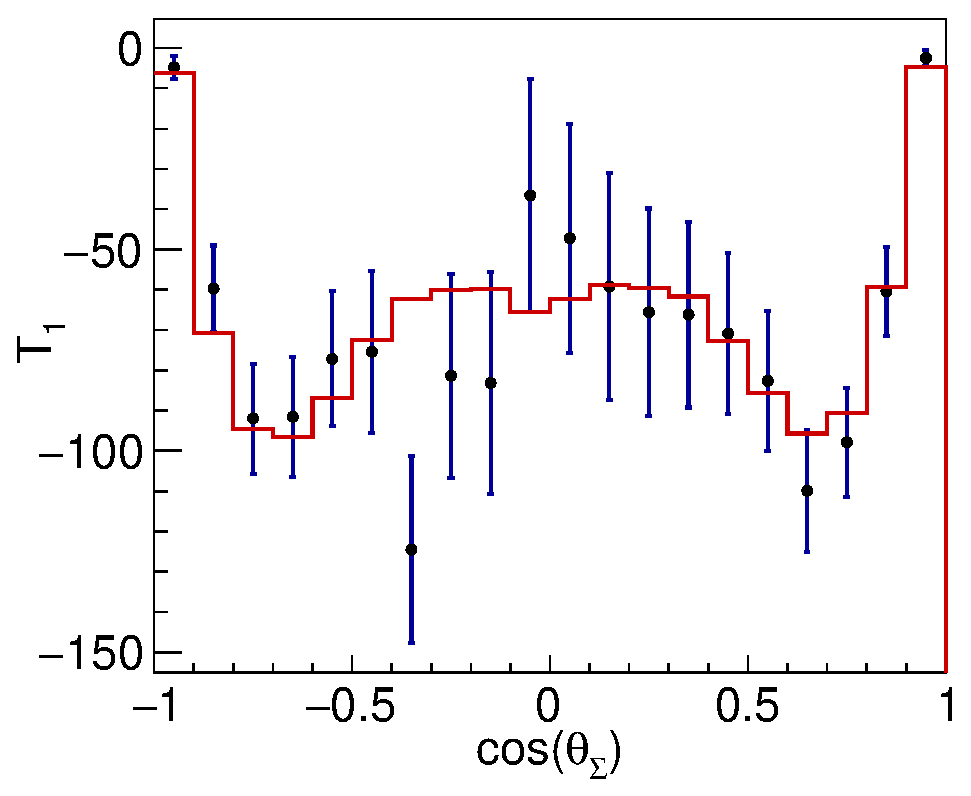
\includegraphics[width = 0.48\linewidth]{jpsi/comDataFit/t1.eps}
        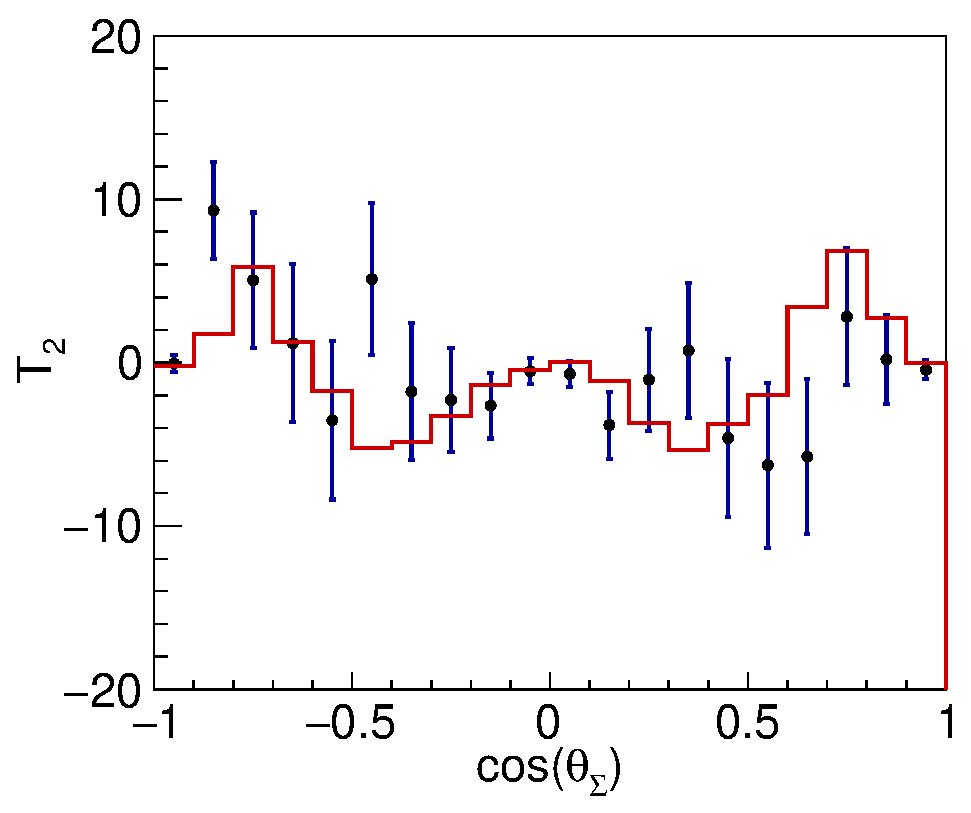
\includegraphics[width = 0.48\linewidth]{jpsi/comDataFit/t2.eps}
    }
    \mbox{%
        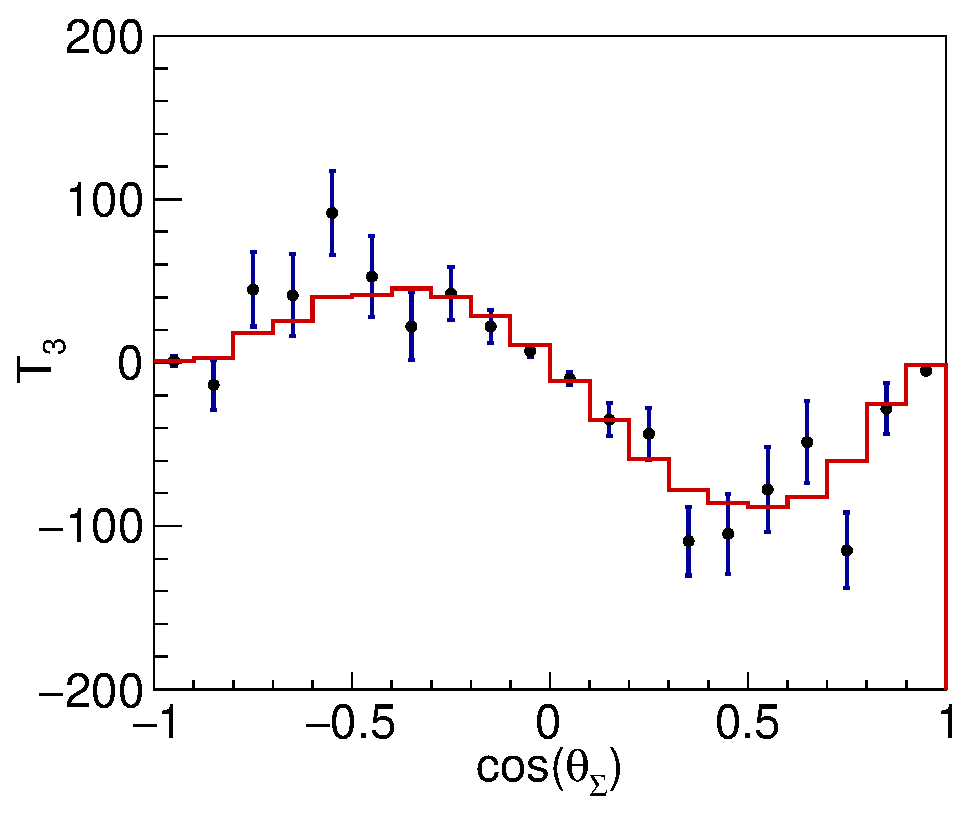
\includegraphics[width = 0.48\linewidth]{jpsi/comDataFit/t3.eps}
        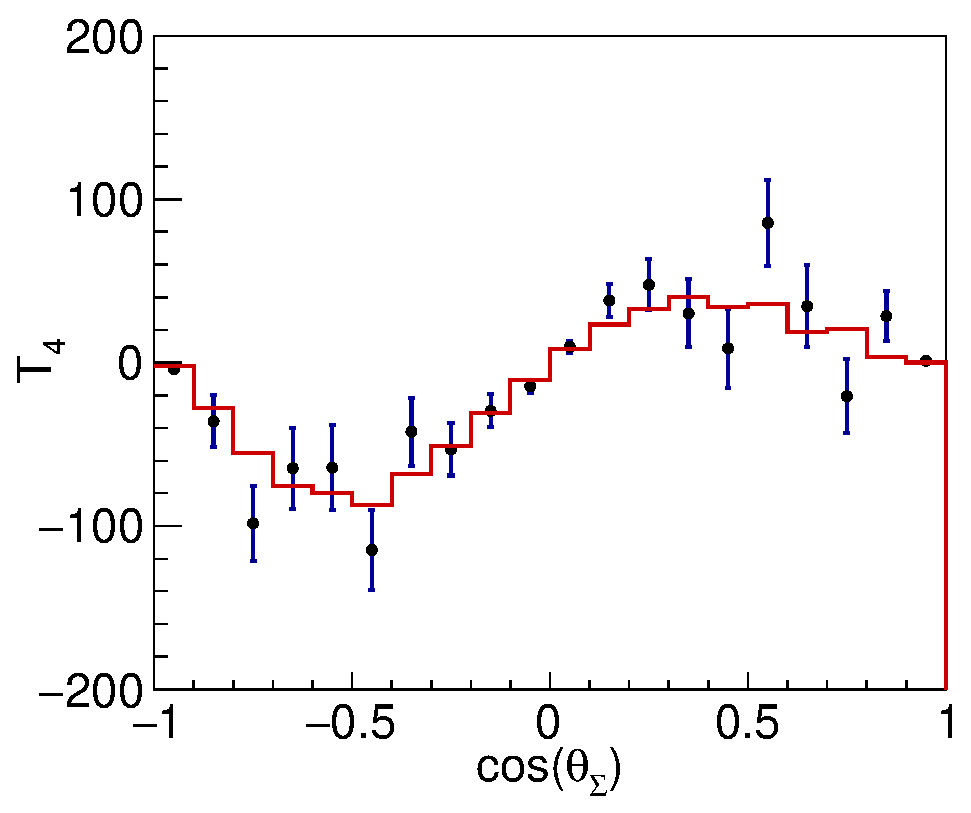
\includegraphics[width = 0.48\linewidth]{jpsi/comDataFit/t4.eps}
    }
    \mbox{%
        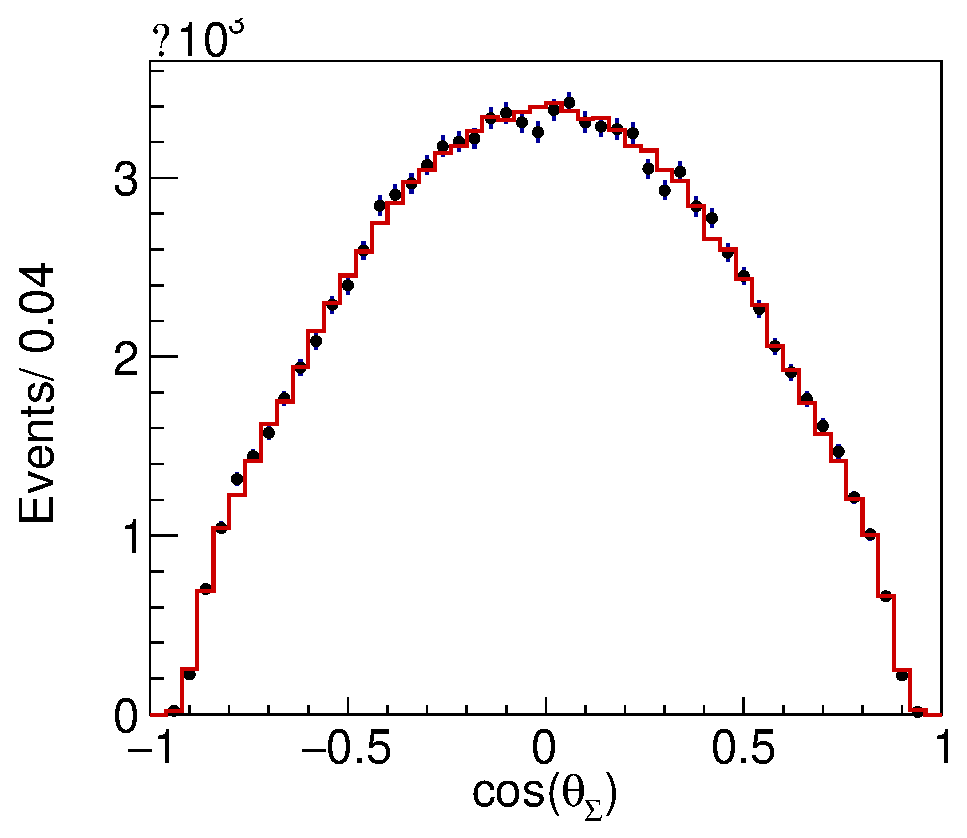
\includegraphics[width = 0.48\linewidth]{jpsi/comDataFit/CosT.eps}
    }
    \caption{数据和蒙特卡洛样本之间特征量的比较。}%
    \label{fig:compare}
\end{figure}


\begin{figure}[htbp]
    \centering
    \mbox{%
       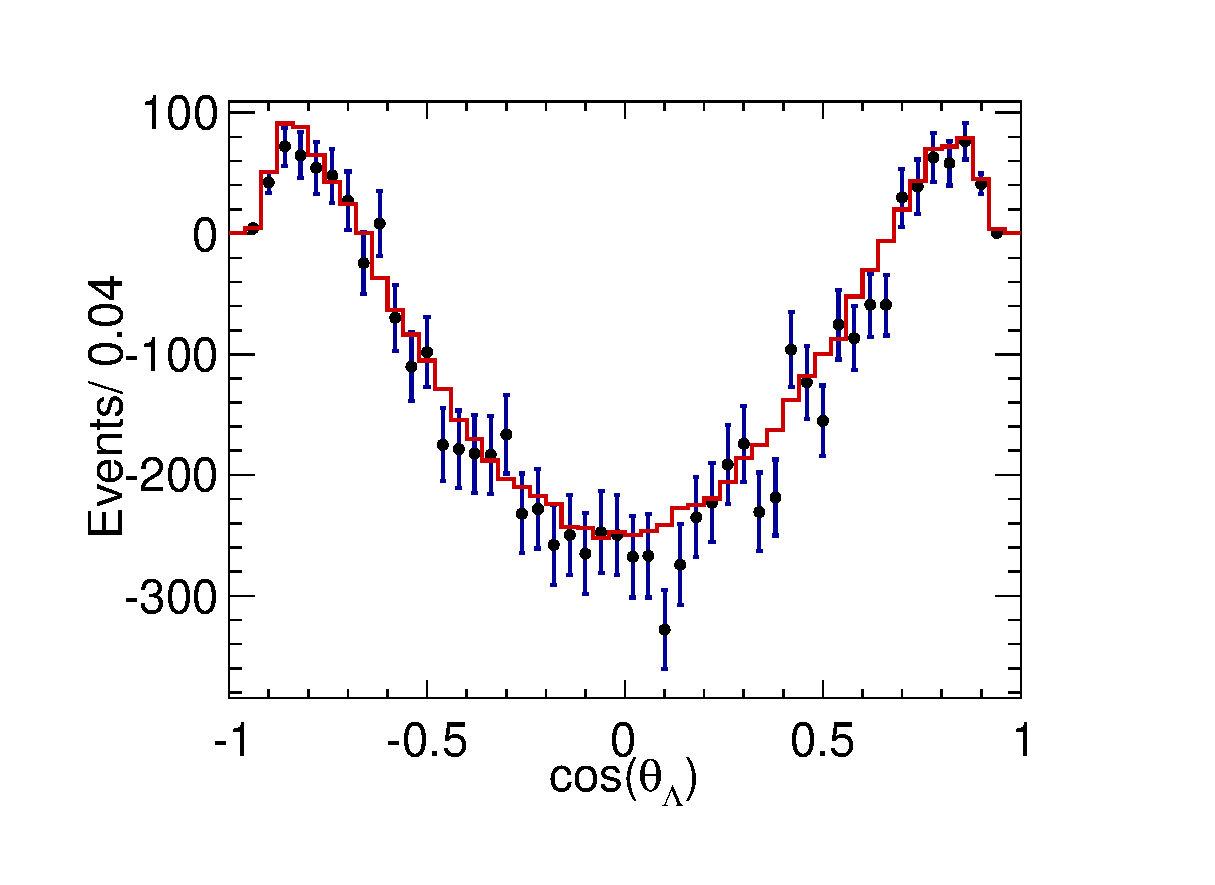
\includegraphics[width = 0.45\linewidth]{jpsi/deteParas/cosL.eps}
       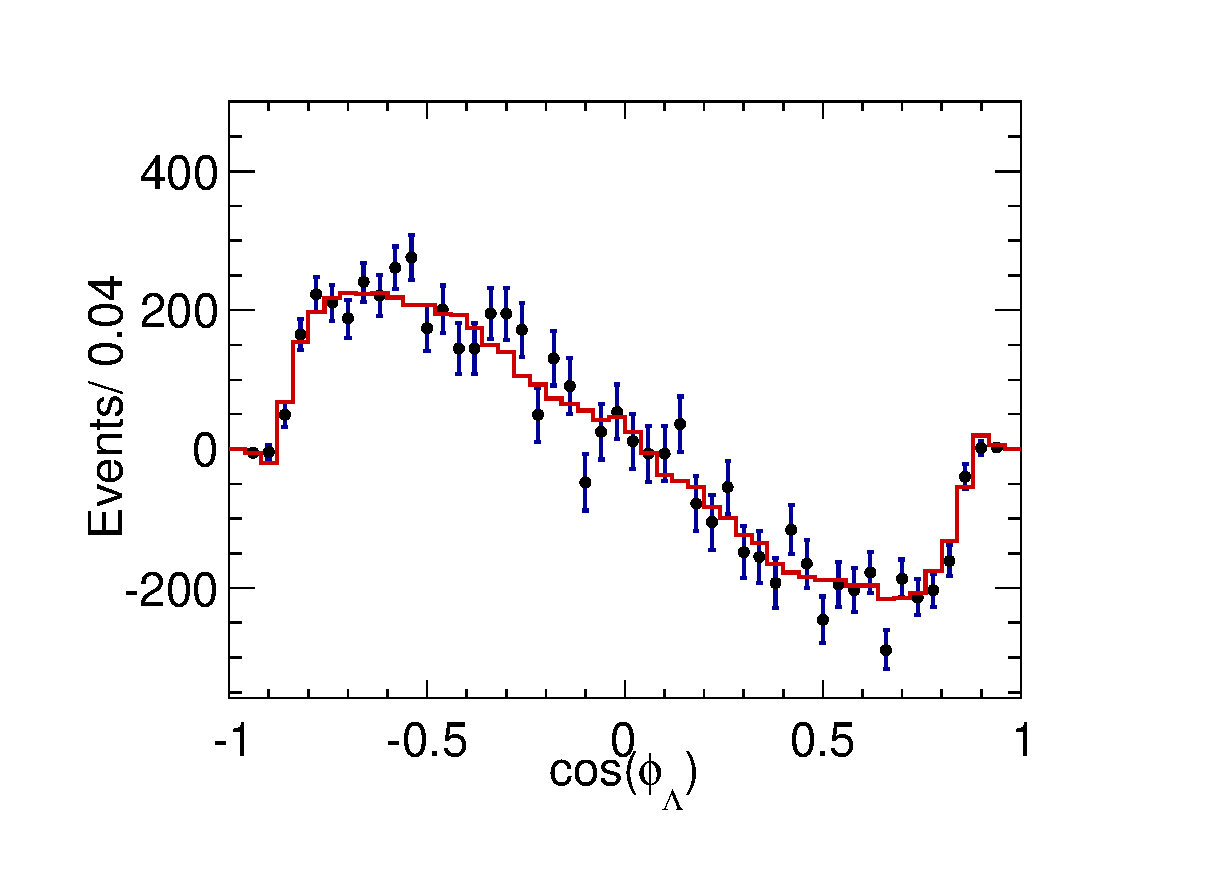
\includegraphics[width = 0.45\linewidth]{jpsi/deteParas/phiL.eps}
   }
   \mbox{%
       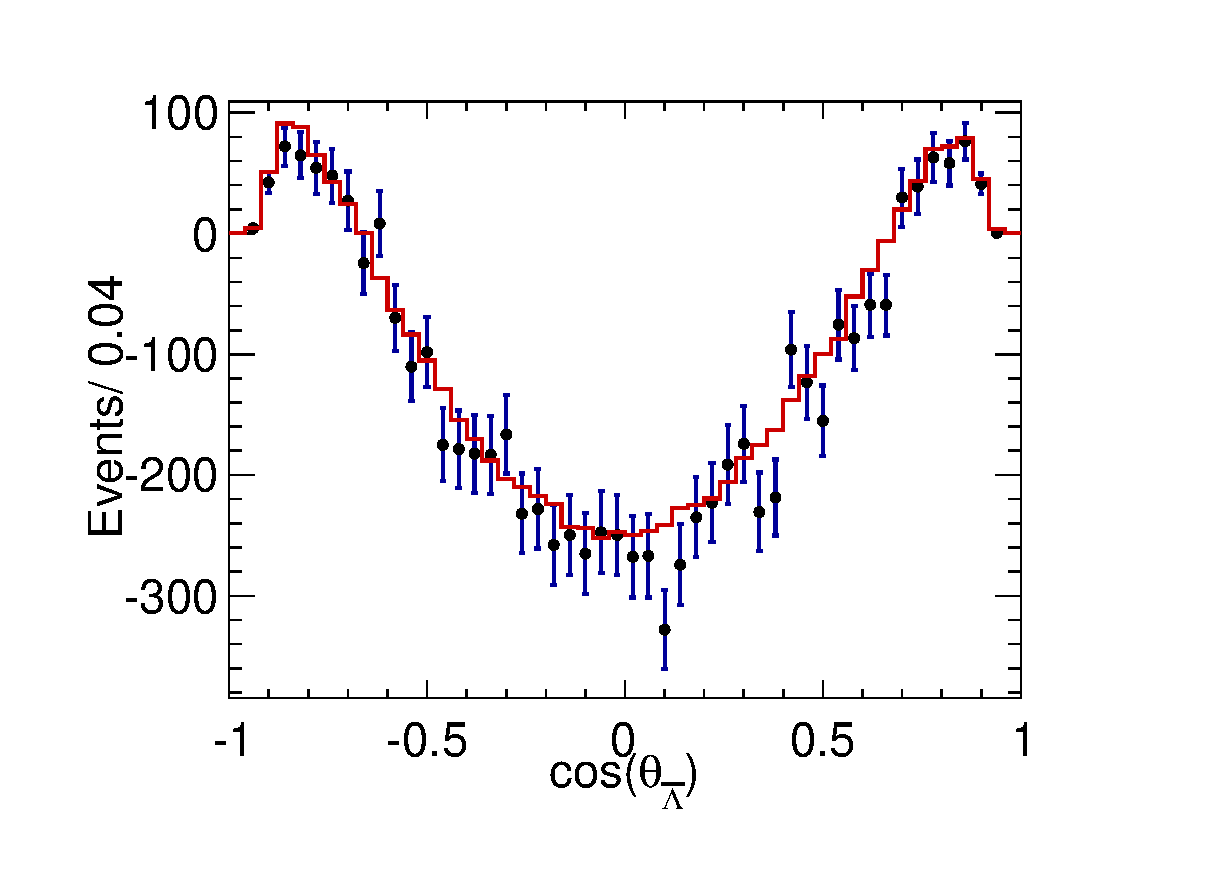
\includegraphics[width = 0.45\linewidth]{jpsi/deteParas/cosLBar.eps}
       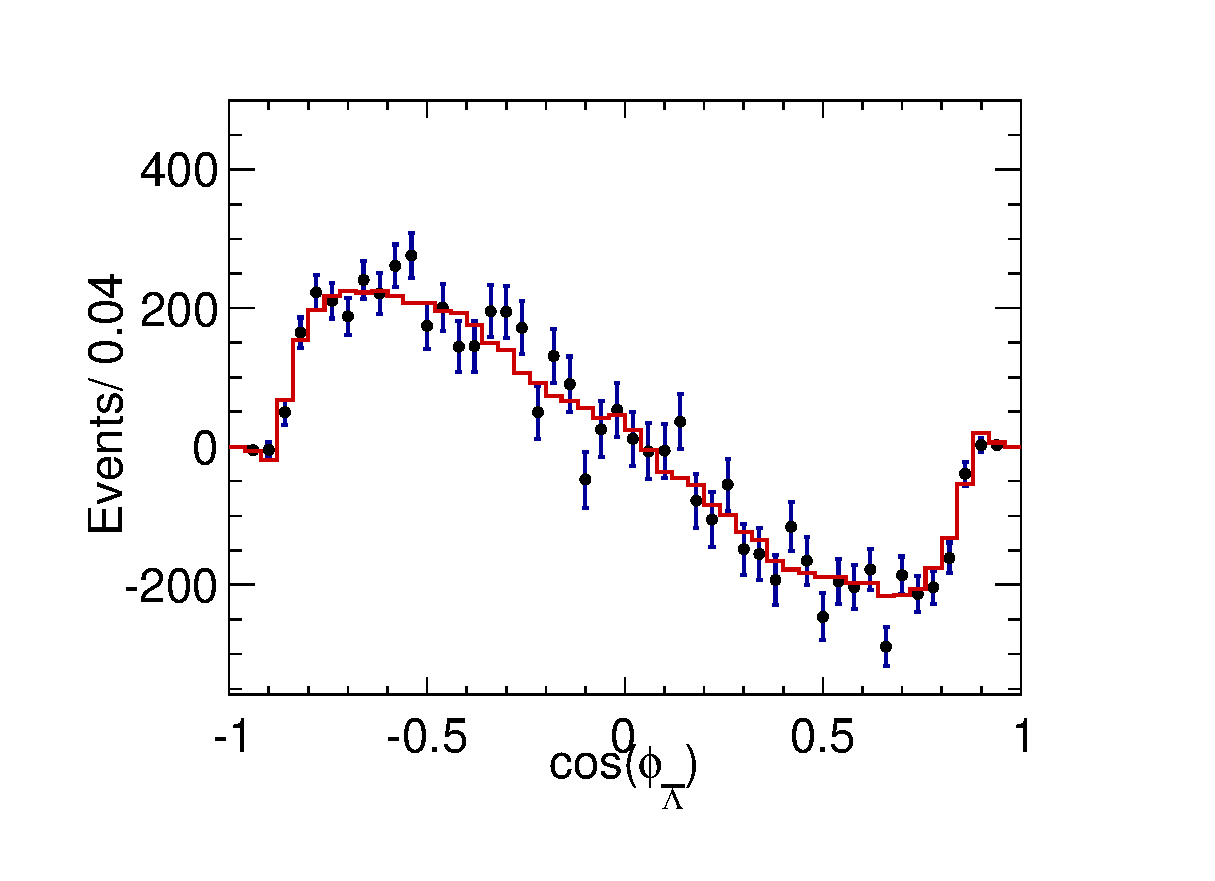
\includegraphics[width = 0.45\linewidth]{jpsi/deteParas/phiLBar.eps}
   }
   \mbox{%
       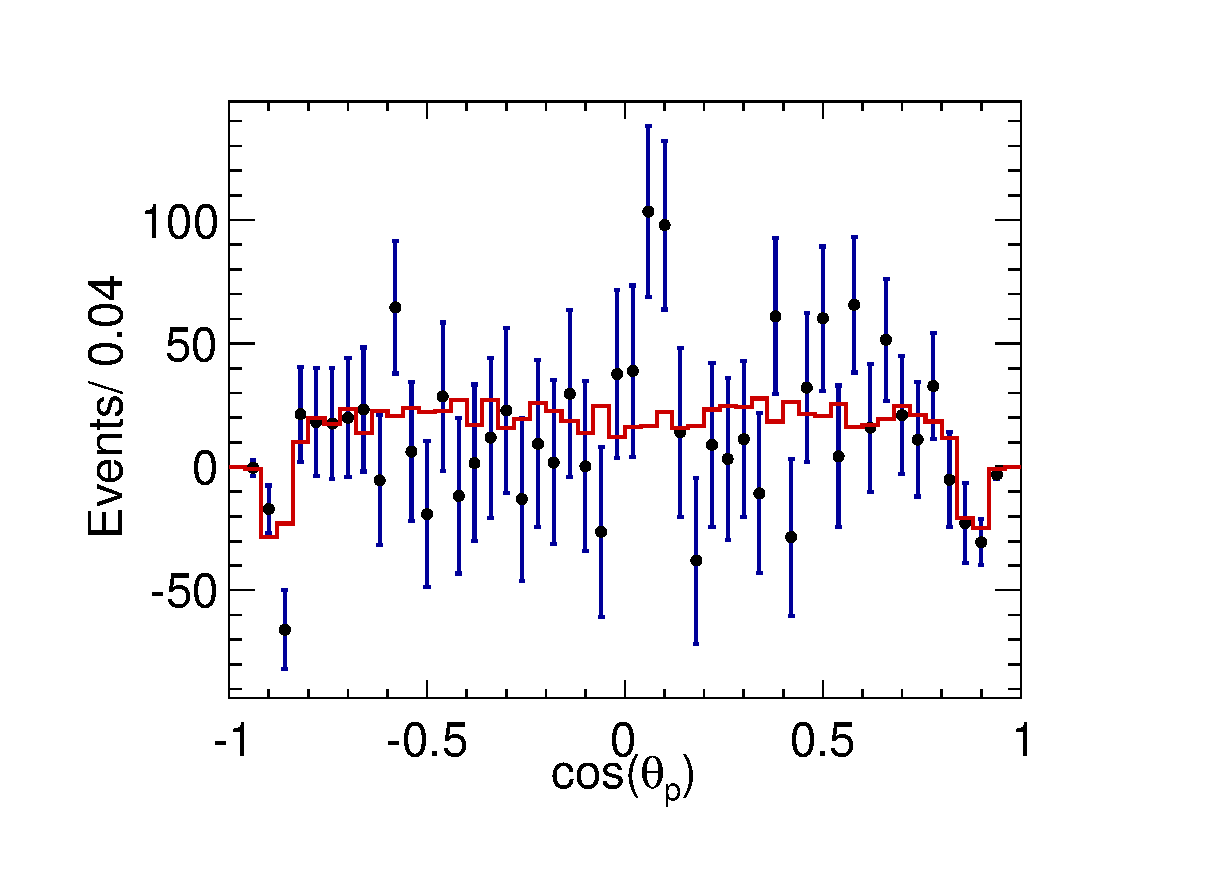
\includegraphics[width = 0.30\linewidth]{jpsi/deteParas/thetaPr.eps}
       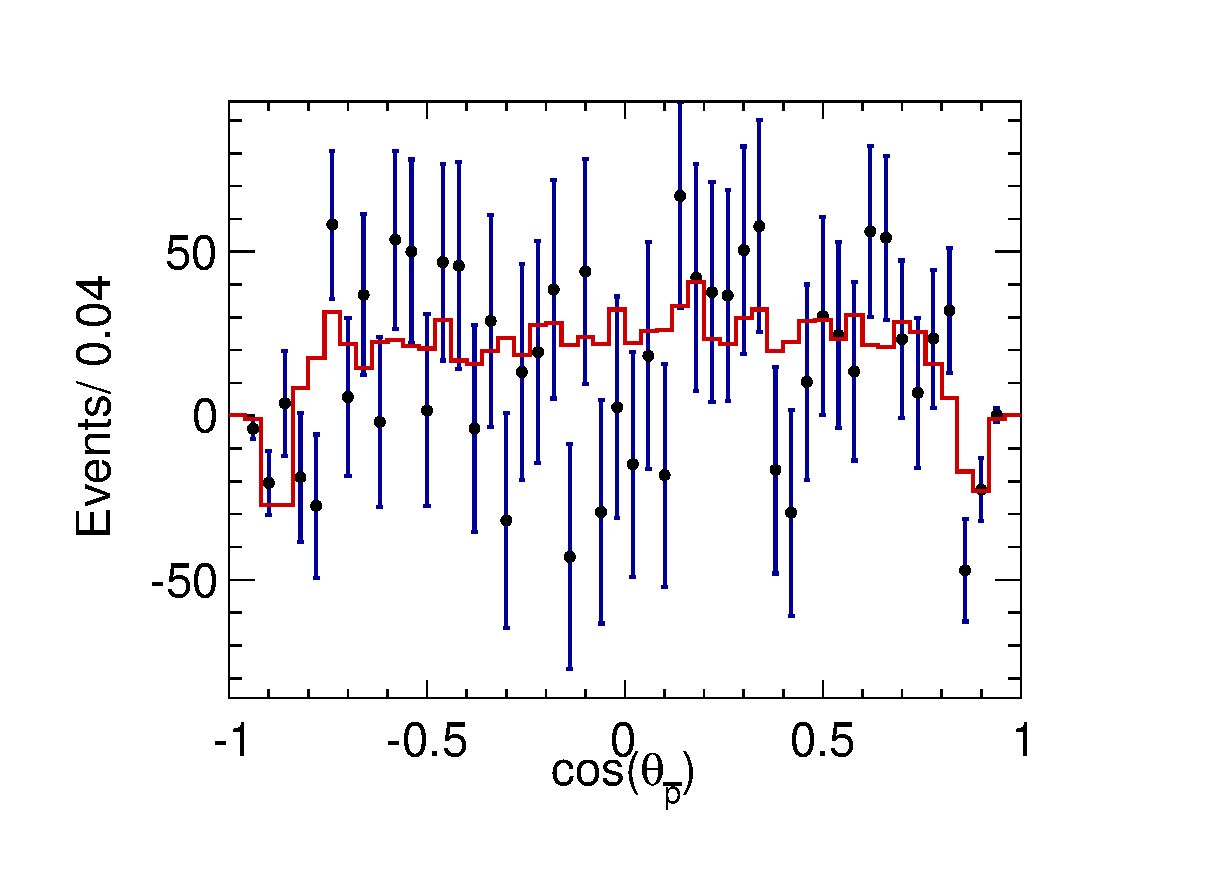
\includegraphics[width = 0.30\linewidth]{jpsi/deteParas/thetaPrBar.eps}
   }
    \caption{数据和信号蒙特卡洛样本之间的比较。}%
    \label{fig:compare2}
\end{figure}
\subsection{寻找CP破坏现象}
在小节\ref{sec:method}中,本文讨论了P宇称破坏以及CP宇称破坏与$\alpha_{\gamma}$
的关系。P宇称破坏将会导致非0的衰变参数$\alpha_{\gamma}$,因此本文要检
验$\alpha_{\gamma}$是否为0。检验的方法为将角分布公式中加入含$\alpha_{\gamma}$的
项,再重复极大似然拟合过程。

\subsubsection*{拟合结果}
按照小节\ref{sec:sigma-likelihood}的步骤,相应的$\alpha_{\gamma}$和
$\bar{\alpha}_{\gamma}$拟合值见表\ref{tab:alphaS}.

\begin{table}[htbp]
    \caption{寻找CP破坏现象的拟合结果。}%
    \label{tab:alphaS}
    \begin{center}
        \begin{tabular} {p{0.5 \linewidth} p{0.3\linewidth}}
            \toprule
            参数 & 拟合结果 \\ 
            \midrule
            $\alpha_{\gamma}$ &  $(0.7 \pm 6.6) \times 10 ^{-3}$ \\ 
            $\bar{\alpha}_{\gamma}$ & $( -7.9 \pm 6.6) \times 10^{-3}$ \\
            \bottomrule
        \end{tabular}
    \end{center}
\end{table}
\subsubsection*{CP破坏强度}
本小节首先定义观测量$O_{CP}$和$O_{C}$来衡量CP破坏和C破坏的强度,具体的定义为
\begin{equation}
    \begin{aligned}
        O_{CP}  =& \frac{\alpha_{\gamma} + \bar{\alpha}_{\gamma}}{2} \\
        O_{C}  =& \frac{\alpha_{\gamma} - \bar{\alpha}_{\gamma}}{2} 
    \end{aligned}
\end{equation}
从上式中可以得到$O_{CP} = (-3.6 \pm 4.8 \pm 0.8)\times 10^{-3}$,
$O_{C} = (0.43 \pm 4.6 \pm 0.8)\times 10^{-3}$,其中的第一项误差为统计误差,
第二项误差为系统误差,后续的章节中将详细讨论系统误差的来源。从中可以看出CP破坏
强度在1$\sigma$内和0一致,并为观测到显著的CP破坏现象,类似了也没有显著的C破坏
现象。

%\subsection{系统误差研究}
\section{系统误差研究}%
\label{sec:sigma0-sys-unc}
系统误差按来源可以分为如下的五种:

\begin{itemize}
    \item 末态带电粒子的寻迹;
    \item 光子的重建;
    \item $\Lambda$和$\bar{\Lambda}$的次级顶点拟合;
    \item 运动学拟合;
    \item 本底估计。
\end{itemize}
每种主要的系统误差来源都可以归为两类,其一通过影响效率函数进而对拟合结果产生
影响,其二则不会影响效率函数本身,但是影响似然函数$S$,比如本底的估计。
第一类系统误差只会影响小节\ref{sec:sigma0-likelihood}中归一化因子$N$的估计,
在计算归一化因子的时候本文选择给予每个蒙特卡洛事例一定的权重以补偿数据和蒙特卡洛样本之间的
效率差异,从而将间接的修正效率函数,具体计算的公式为
\begin{equation}
    \label{eq:vary-weight-sigma0}
    N' = \frac{1}{n}  \sum_{i}^{MC} weight_{i} \cdot 
    \mathcal{P}(\vec{\theta_{i}}; \vec{\alpha}),
\end{equation}
式中$weight_{i}$代表第$i$个蒙特卡洛样本的权重,应如此计算
\begin{equation}
    weight  \equiv \frac{\epsilon_{\rm data}}{\epsilon_{\rm MC}} ,
\end{equation}
其中的$\epsilon_{\rm data}$和$\epsilon_{\rm
MC}$分别是数据和蒙特卡洛中的效率函数。这些效率一般从控制样本中得到,
比如质子的寻迹效率。
第二类系统误差不会改变效率曲线的形状,但也会影响拟合的结果,比如本底的估计。
一般通过估计策略的变动拟合结果也随之改变,因此本文采用变化策略,把拟合结果的变动
作为系统误差。在下节将讨论具体的方法。
\subsection{带电粒子的寻迹}%
\label{sec:Tracking-unc-sigma0}
末态的带电粒子种类包括质子和$\pi$介子。一般需要通过控制样本来研究带电粒子的寻迹
效率。控制样本选取的原则包括:大样本、低本底。研究质子寻迹效率的一个理想样本
是:
$J/psi \to p \bar{p} \pi^{+} \pi^{-}$。研究的精神是:
\begin{itemize}
    \item 用三个带电末态$\bar{p} \pi^{+} \pi^{-}$标记质子,这样得到的被标记质子
        就是所谓的控制样本。由于带电粒子的动量分辨好,本底低,因此被标记质子的
        运动学信息能够被精确的得到。另一方面,很容易通过拟合丢失不变质量谱
        确定质子的数目。
    \item 根据被标记质子的运动学信息去寻找一条与之相符的带电径迹。一般常常利用
        飞行方向的信息,两者夹角小于20度认为寻迹正确。
\end{itemize}
宋娇娇博士对质子和$\pi$介子的寻迹效率进行了研究\cite{PID:jiaojiao},
在她研究得到的效率的基础上,本文对式\ref{eq:vary-weight-sigma0}中的权重进行相应
的变动。本文把相空间积分蒙特卡洛样本按质子和$\pi$介子的动量和极角划分成
若干区间,其中动量区间的宽度为100 MeV$/c$,极角 ($\cos\theta$)的区间宽度为0.2。
本文假设任意一个区间内的权重因子服从高斯分布,$\sigma$按误差传递公式确定。
为了确定修正带来的误差,本文选择做多次实验,每次实验的中的每个区间内的权重因子
均按高斯分布进行随机抽取,最终得到一系列拟合结果。经过400次实验后,得到的拟合
结果见图\ref{fig:fit-value-track}。如图所示,拟合结果的中心值应服从正态分布,
为了验证这一点,本文用高斯函数对这400次实验做了拟合,蓝色的实线是拟合的结果。
本文选择把高斯函数的中心值作为经过径迹效率修正后的报告值,高斯函数的$\sigma$
作为径迹效率修正的系统误差,这项误差总结在表\ref{tab:unc-track-sigma0}中。

% /besfs/groups/jpsi/jpsigroup/user/maxx/Jpsi/SS/664/noDangCut/Uncertainty/trackingAndPid/
\begin{figure}[htbp]
    \centering
    \mbox{%
        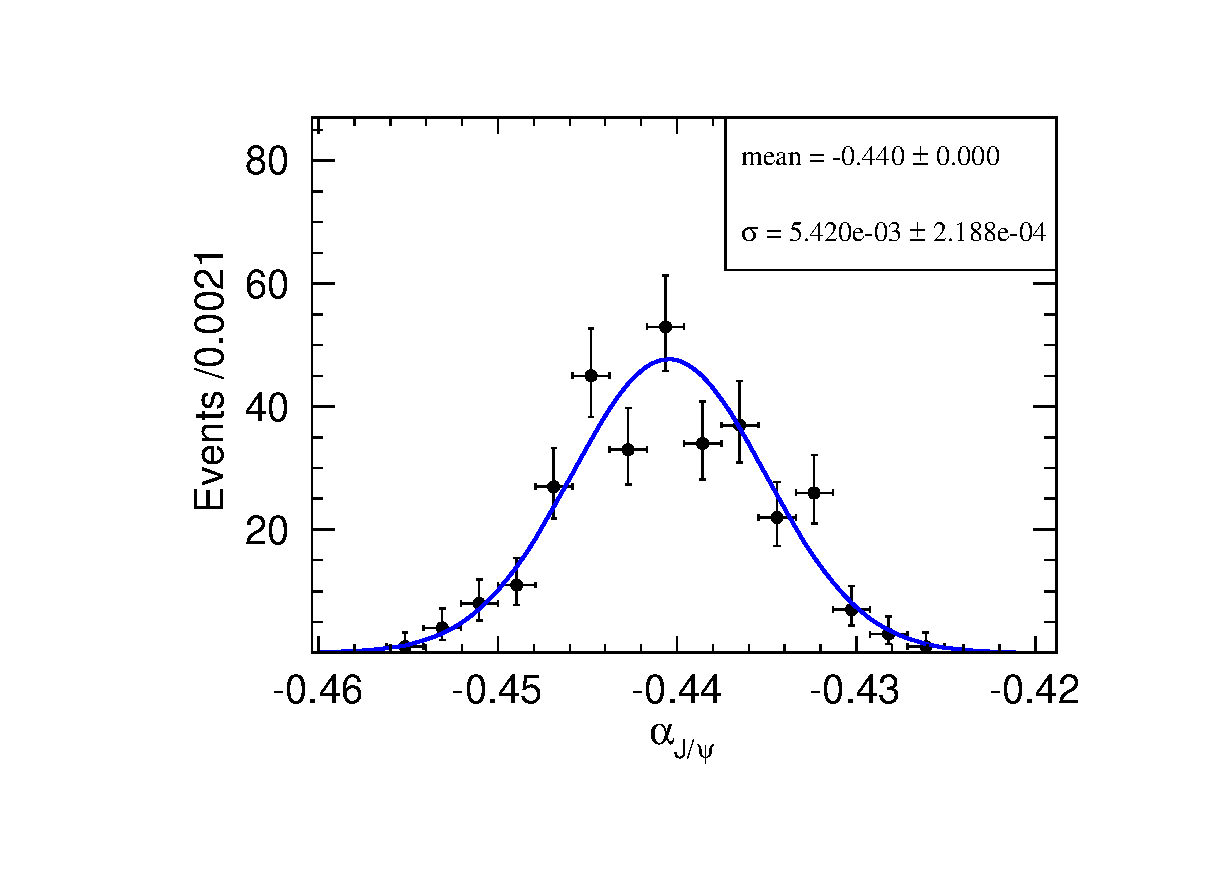
\includegraphics[width = 0.48\linewidth]{jpsi/unc/trkalpha.eps}
        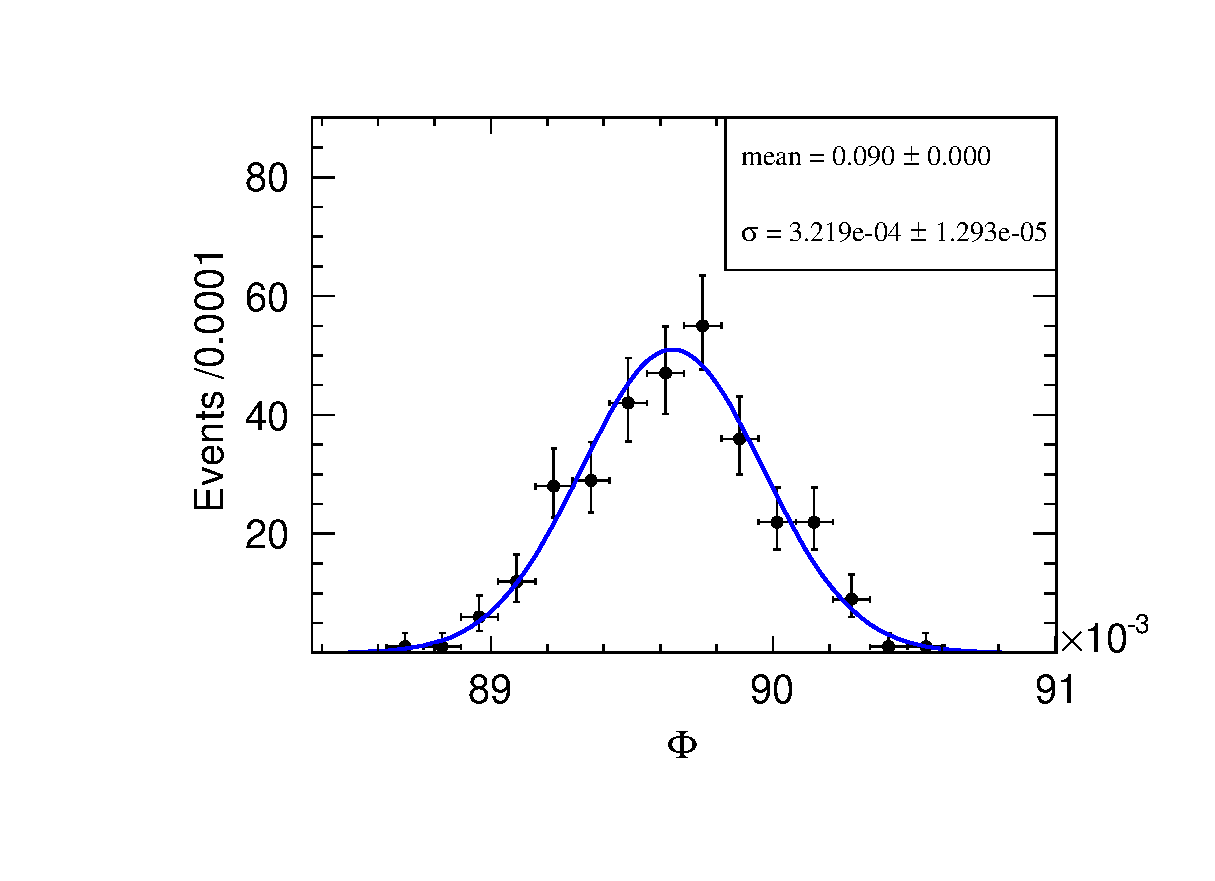
\includegraphics[width = 0.48\linewidth]{jpsi/unc/trkphi.eps}
    }
    \mbox{%
        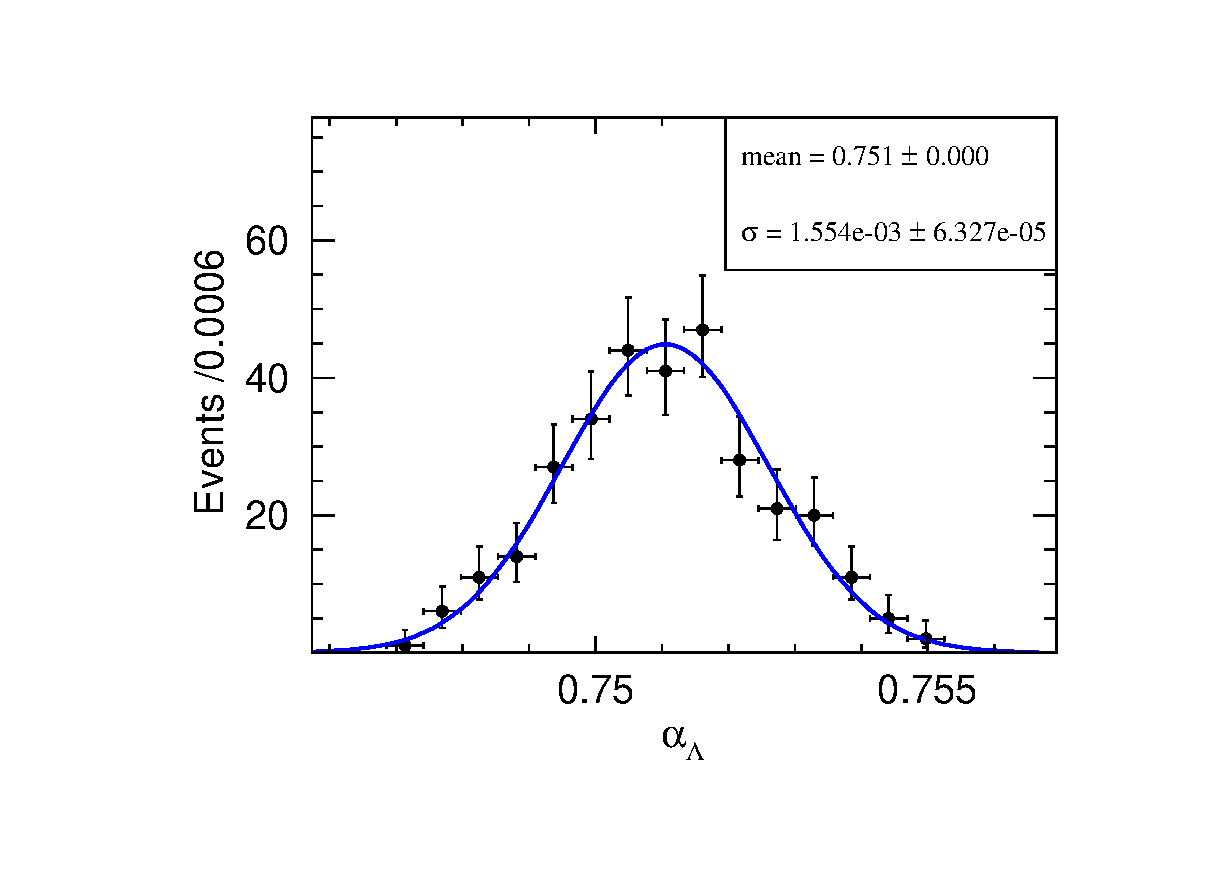
\includegraphics[width = 0.48\linewidth]{jpsi/unc/trkalphaL.eps}
        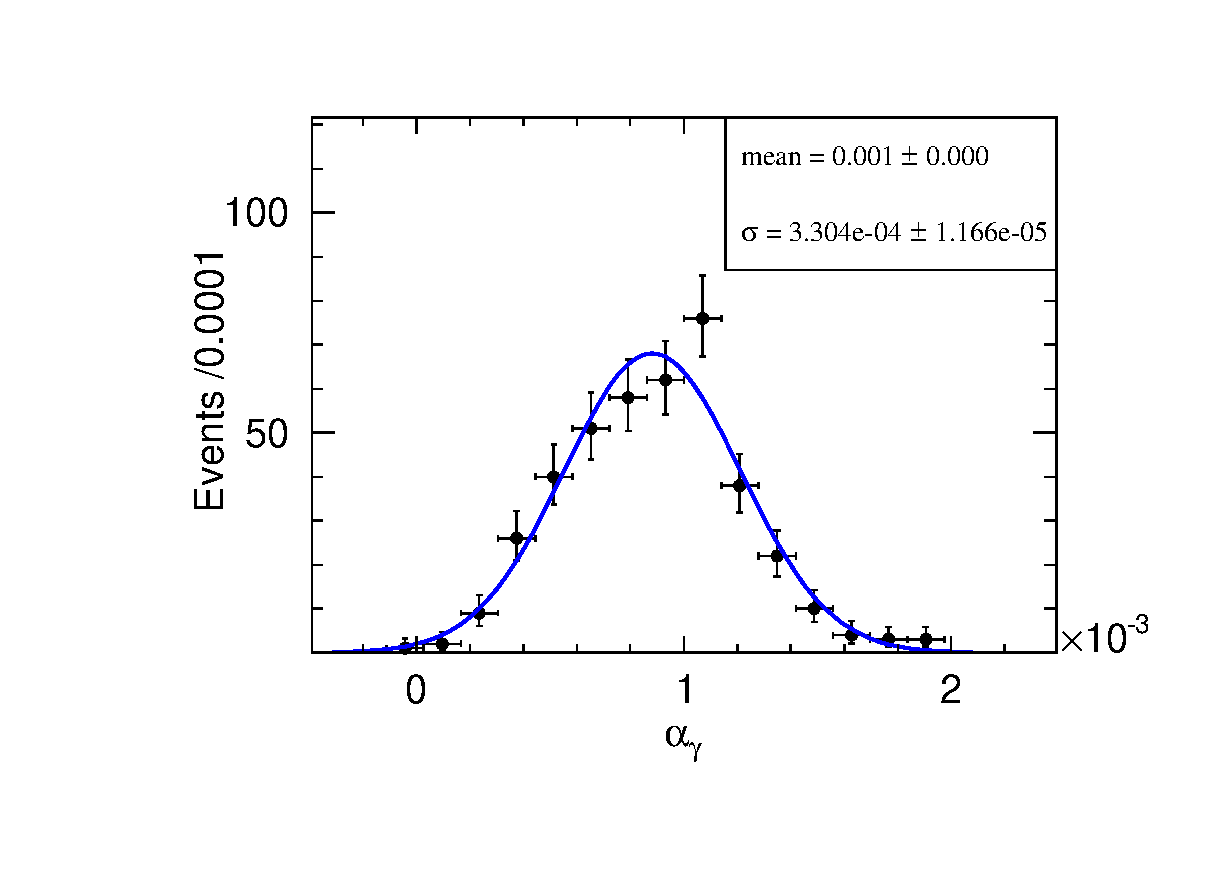
\includegraphics[width = 0.48\linewidth]{jpsi/unc/trkalphagamma.eps}
    }
    \mbox{%
        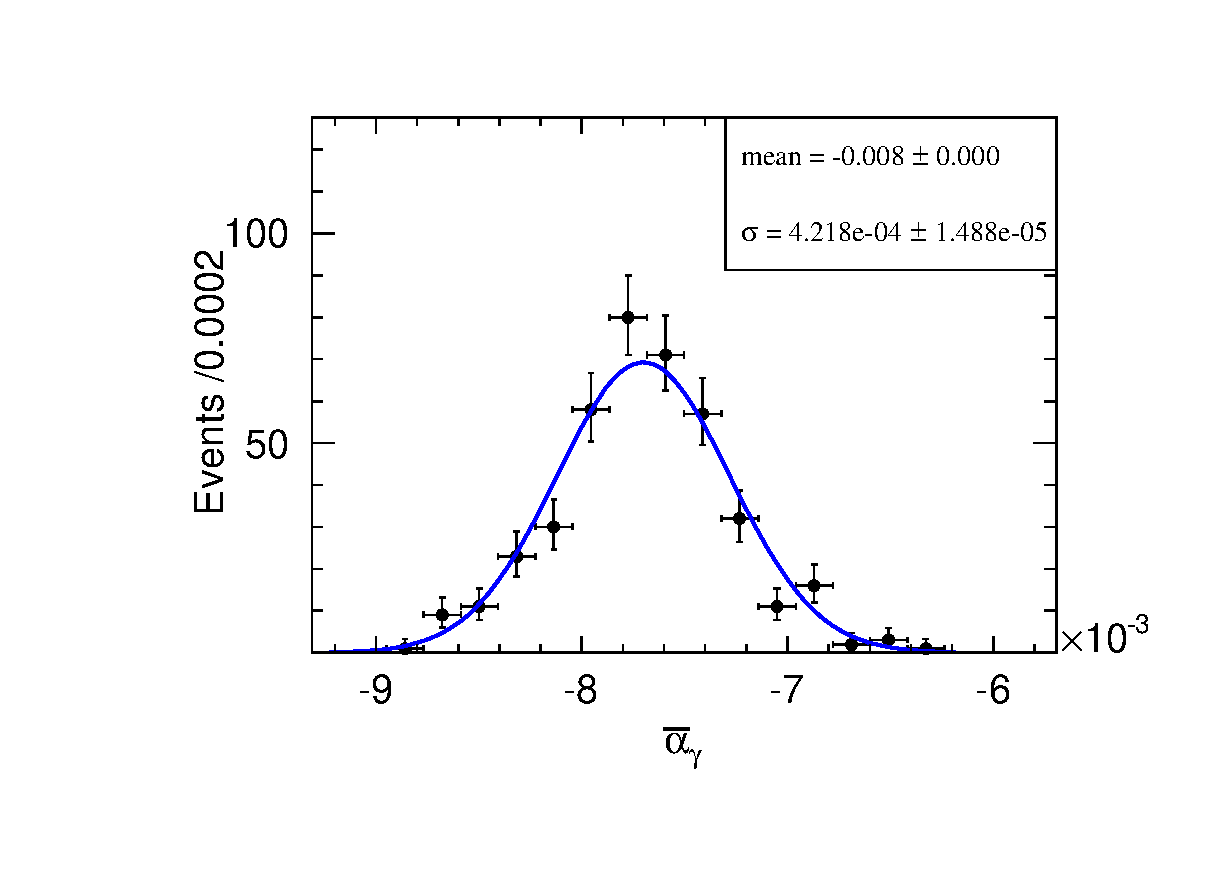
\includegraphics[width = 0.48\linewidth]{jpsi/unc/trkalphagammaBar.eps}
    }
    \caption{%
        随机变动参数$weight$得到的多次实验结果。本文对图中400次拟合结果做了拟合。
        蓝色的实线表示拟合的结果,相关的参数结果标注在图的右上角。
    }%
    \label{fig:fit-value-track}
\end{figure}


\begin{table}[htbp]
    \caption{寻迹效率修正的系统误差。}%
    \label{tab:unc-track-sigma0}
    \begin{center}
        \begin{tabular} {p{0.5 \linewidth} p{0.3 \linewidth}}
            \toprule 
            参数 & 系统误差 (\%) \\
            \midrule
            $\alpha_{J/\psi}$  & 1.3 \\
            $\Phi$             & 0.36 \\
            $\alpha_{\Lambda}$ & 0.21 \\
            \bottomrule
        \end{tabular}
    \end{center}
\end{table}

\subsection{光子重建}%
\label{sec:photon-rec-Sigma0}
光子重建效率与极角和能量有关,Vindy博士对光子重建的效率进行了系统的研究,在他
的工作的基础,本文按光子的极角和能量对效率曲线进行了修正,并得到了相应的系统
误差。在Vindy博士研究成果的基础上,本节对式\ref{eq:vary-weight-sigma0}中
的$weight$进行相应的随机变动。做了400变动后,得到的拟合参数的分布
如图\ref{fig:fit-value-photon}所示,采取和小节\ref{sec:Tracking-unc-sigma0}
相同的策略得到的系统误差总结在表\ref{tab:unc-photon-Sigma}中。
% /besfs/groups/jpsi/jpsigroup/user/maxx/Jpsi/SS/664/noDangCut/Uncertainty/gammaRec/
\begin{figure}[htbp]
    \centering
    \mbox{%
        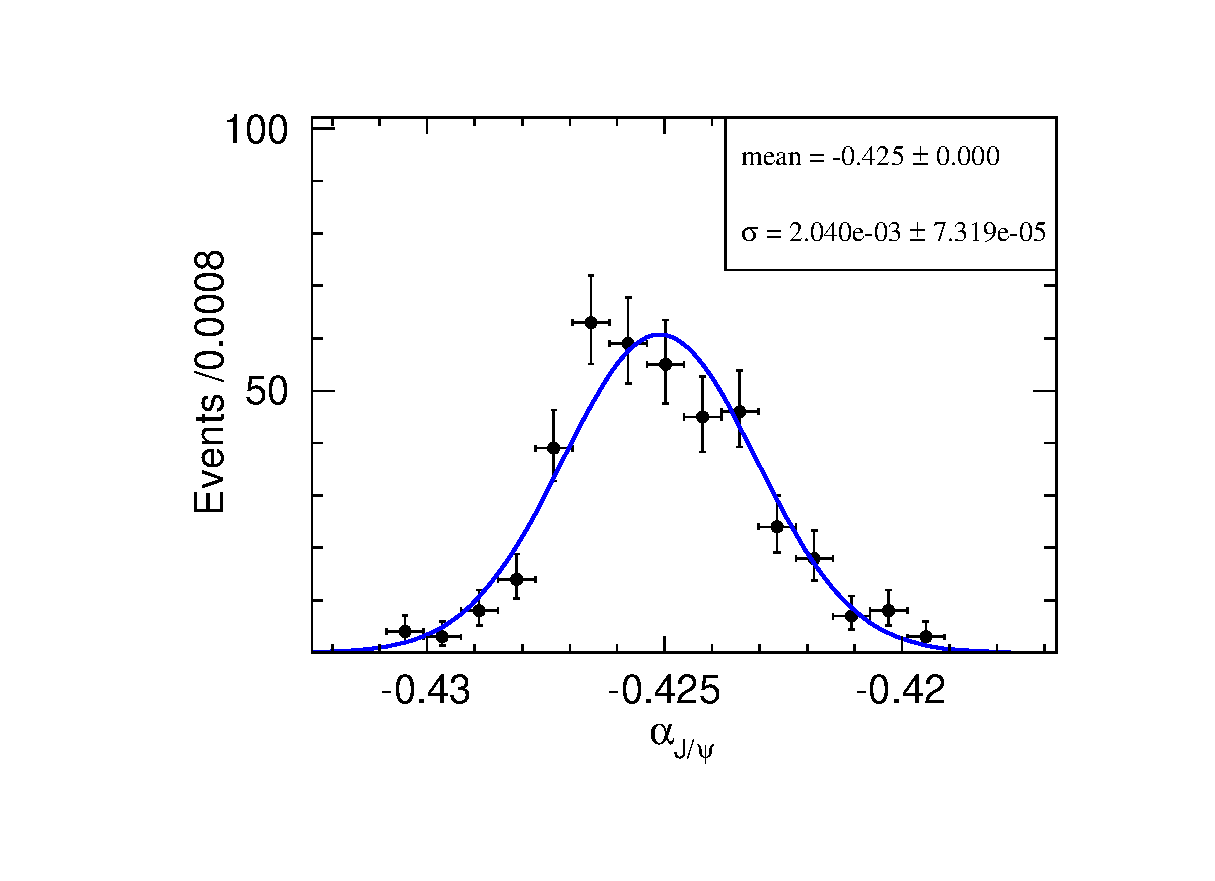
\includegraphics[width = 0.48\linewidth]{jpsi/unc/photonalpha.eps}
        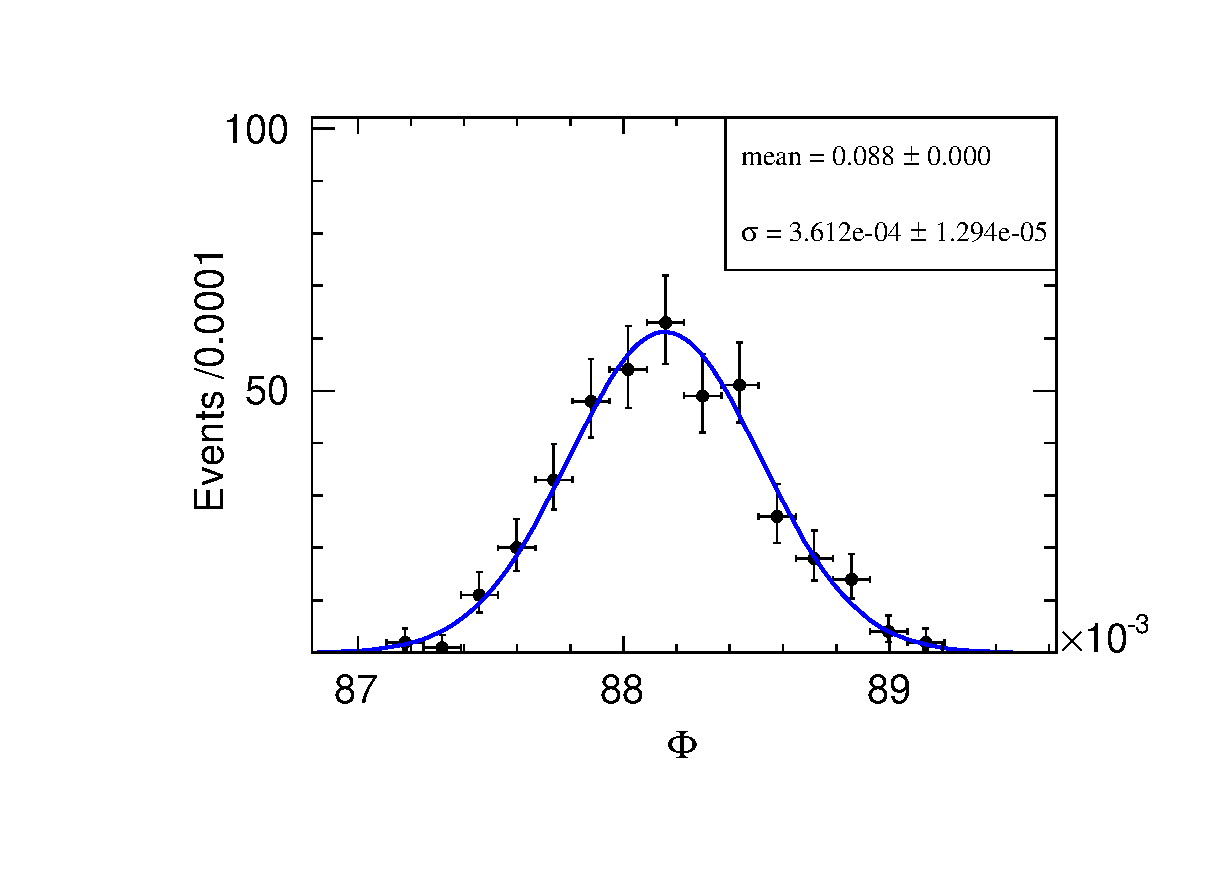
\includegraphics[width = 0.48\linewidth]{jpsi/unc/photonphi.eps}
    }
    \mbox{%
        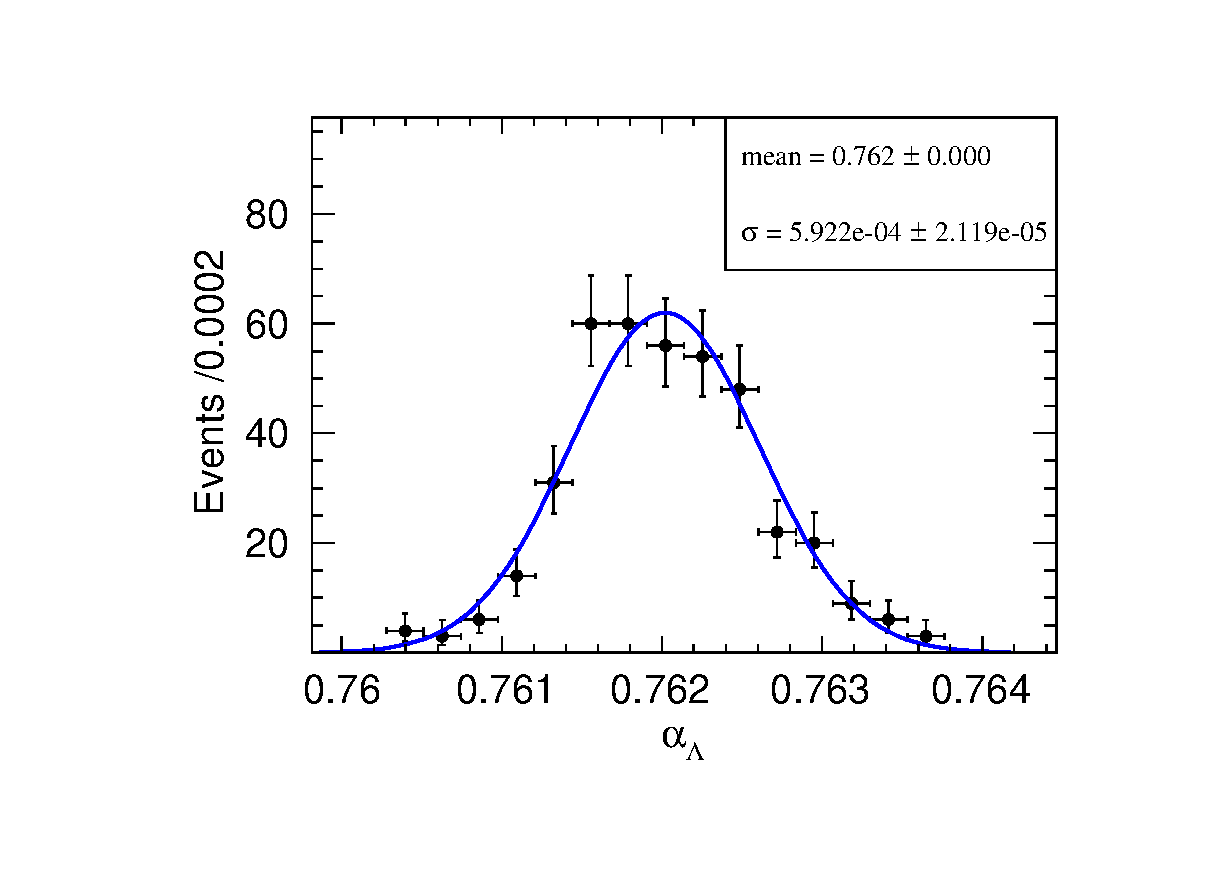
\includegraphics[width = 0.48\linewidth]{jpsi/unc/photonalphaL.eps}
        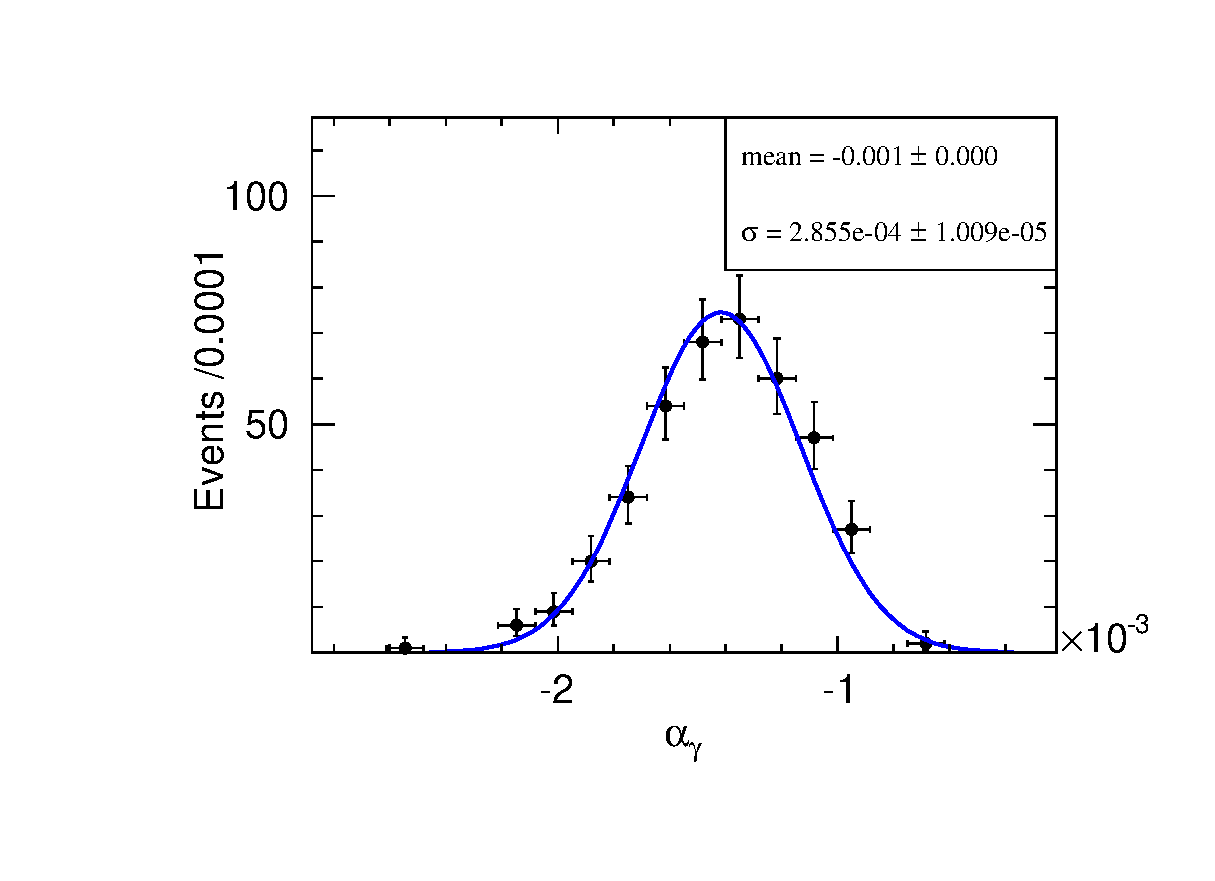
\includegraphics[width = 0.48\linewidth]{jpsi/unc/photonalphagamma.eps}
    }
    \mbox{%
        \includegraphics[width = 0.48\linewidth]{jpsi/unc/photonalphagammaBar.eps}
    }
    \caption{%
        对光子重建效率进行400次加权测试得到的拟合参数分布。带误差棒的黑色的
        带误差棒的点表示拟合的结果,蓝色的实线为用高斯函数拟合的结果。
    }%
    \label{fig:fit-value-photon}
\end{figure}

\begin{table}[htbp]
    \caption{光子重建带来的系统误差总结。}%
    \label{tab:unc-photon-Sigma}
    \centering
    \begin{tabular} {p{0.5 \linewidth} p{0.4 \linewidth}}
        \toprule 
        衰变参数 & 系统误差 (\%) \\
        \midrule
        $\alpha_{J/\psi}$  & 0.48 \\
        $\Phi$             & 0.41 \\
        $\alpha_{\Lambda}$ & 0.78 \\
        \bottomrule
    \end{tabular}
\end{table}

\subsection{$\Lambda$的次级顶点重建}
为了研究$\Lambda$的次级顶点重建的效率,本节挑选了控制样本$J/\psi 
\to pK^{-} \bar{\Lambda}$及$J/\psi \to \Lambda \bar{\Lambda}$来确定数据和
蒙特卡洛样本中的重建效率。加上详细的叙述。

\subsection{运动学拟合}
本节选择控制样本$J/\psi \to p \bar{p} \pi^{+}\pi^{-}\pi^{0}$来确定运动学拟合
的效率曲线,这个控制样本的特点是末态和信号高度相同,能够有效的揭示出数据
和蒙特卡洛之间的差异。加上描述。

\subsection{本底的影响}
为了确定本底带来的影响,本节采取去掉公式\ref{eq:final-likehood}中的本底项
重新进行拟合并把和保留本底项的结果进行比较,两者之间的差异作为系统误差。

%\subsection{系统误差小节}
至此所有的系统误差都得到了精细的研究,每项的系统误差和总的系统误差见
表\ref{tab:unc-summary}.

\begin{table}[htbp]
    \caption{系统误差的总结表。}%
    \label{tab:unc-summary}
    \centering
    \begin{tabular} {p{0.3 \linewidth} p{0.1\linewidth} p{0.1\linewidth} 
        p{0.1\linewidth} p{0.1\linewidth} p{0.1\linewidth} }
        \toprule
        \multirow{2}{*} {来源}
        & \multicolumn{5}{c}{误差 (\%)} \\ 
        \cline{2-6}
        & $\alpha_{J/\psi}$ & $\Phi$ & $\alpha_{\Lambda}$ 
        & $\alpha_{\gamma}*$ & $\bar{\alpha}_{\gamma}*$ \\
        \midrule
        寻迹 & $1.3$ & $0.36$ & $0.21$  & $0.3 \times 10^{-4}$ 
        & $4.2 \times 10^{-4}$ \\
        光子重建 & $0.48$ & $0.41$ & $0.78$
        & $2.8 \times 10^{-4}$ & $2.8 \times 10^{-4}$\\
        $\Lambda$的次级顶点重建 & $2.8$ & $0.53$ & $0.37$ 
        & $4.2 \times 10^{-4}$ & $4.2 \times 10^{-4}$ \\
        运动学拟合 & $2.0$ & $0.57$ & $0.41$
        & $6.0 \times 10^{-4}$ & $5.9\times 10^{-4}$ \\
        本底估计 & $0.80$ & $0.58$ & $0.07$
        & $7.6 \times 10^{-4}$ & $7.9 \times 10^{-4}$ \\
        \midrule
        总和 & $3.8$ & $1.1$ & $1.0$  & $1.2 \times 10^{-3}$ & 
        $1.2 \times 10^{-3}$ \\
        \bottomrule
    \end{tabular}
\end{table}

% ====================================================
%   Copyright (C)2019 All rights reserved.
%
%   Author        : Xin-Xin Ma
%   Email         : xxmawhu@163.com
%   File Name     : sigma0Decay.tex
%   Last Modified : 2020-01-09 18:42
%   Describe      :
%
% ====================================================%
\chapter{研究$\Sigma^{0}$的达利兹衰变}
\section{简介}%
\label{sec:introduction-dalitz-decay}
在1957年$\Sigma^{0}$首次被发现\cite{1957:desoh,Plano1957},
同时$\Sigma^{0}$的质量被确定为$1187 \pm 4{\rm MeV}/c^{2}$,随后H. Courant和
P. Franzini利用$\Sigma^{0}$的末态粒子角分布信息无可争议的确定了$\Sigma^{0}$的
自旋为$1/2$\cite{Plano1957}。随后的几年里,许多实验组对$\Sigma^{0}$进行了一系列的
研究,很快$\Sigma^{0}$的达利兹被发现,从而确定了$\Sigma^{0}$的宇称为
正\cite{Courant:1963zzd,AlffSteinberger:1965zz}。由于实验精度的限制和实验手段的
有限性,直到1977年SPEC实验组才通过$\Sigma^{0}$在核子近场中的Primakoff效应首次
测量了其寿命$5.8\pm 1.3 \times 10^{-20} s$\cite{Dydak:1976dn},9年后SPEC实验
组提高了测量精度$7.4\pm 0.7 \times 10^{-20}
s$\cite{Petersen:1986fi,Devlin:1986hm}。然而我们对$\Sigma^{0}$的其他性质的研究仍
知之甚少,至今尚对$\Sigma^{0}$的磁矩大小的实验数据是空白的。虽然早在1965年
$\Sigma^{0}$的达利兹衰变就被观测到了,但是其分支比的大小还是个未知数。
衰变$\Sigma^{0}  \to \Lambda e^{+} e^{-}$的分支比和$\Sigma^{0}$的电磁形状因子紧密相关,
其分支比的大小的引起了理论家的广泛讨论\cite{Feinberg:1958zz,Michel:1965zz,Sidhu:1972rx,
Mani:1974wt,Abers:1977dc,Husek:2019wmt},1957年,G.Feinberg首次从理论上预言
$B(\Sigma^{0} \to \Lambda e^{+} e^{-}) = 5.45 \times 10^{-3}$,考虑到辐射修正后分支比
增大1\%左右\cite{Sidhu:1972rx}。目前理论上的预言的分支比已经达到了11\%的精度,这将有助于
检验标准模型以及寻找潜在的新物理的贡献。在2016年,一种 奇特的现象在Be的激发态和基态之间的跃迁过程
被发现\cite{Krasznahorkay:2015iga},信号显著性超出了5倍$\sigma$。一个新的中性的矢量中间传播子有助于
解释这个实验现象,这个玻色子被叫做$X(17)$,其质量被确定为$16.70 \pm 0.36 {\rm MeV}/c^{2}$。在其他的实验
中,寻找到这个新粒子$X(17)$将提供更加坚实的证据,有助于在粒子物理学中掀起新的革命。
在乔从丰教授等人预言\cite{Jiang:2018uhs}BESIII会产生52个$J/psi \to X(17) \gamma$事例,这急需BESIII实验对
$J/\psi$数据进行分析确认或否定$X(17)$的存在。作为$uds$夸克组成的核子,$\Sigma^{0}$是$\Lambda$的激发态,两者之
间的能级差为$76.959 \pm 0.023 {\rm MeV}$,这与$Be^{*}$和$Be$之间
的能级差大致相当,这提供了一个验证文献\cite{Krasznahorkay:2015iga}的结果的重要平台。
如果$X(17)$存在,并且在核子之间的耦合具有普适性,那么实验上将观测到$\Sigma \to \Lambda e^{+} e^{-}$的分支比
的增强,精确测量这个分支比有助于确定$X(17)$和核子的耦合常数。

\subsection{衰变机制}
在标准模型的框架内,$\Sigma^{0} \to \Lambda e^{+} e^{-}$是电磁相互作用主导的,
弱中性流的贡献约为$10^{-6}$。
\begin{figure}[htbp]
    \centering
    \mbox{%
    \includegraphics[width =0.8\linewidth]{figures/Sigma/intr/LO.eps}
    }
    \caption{%
        $\Sigma^{0} \to \Lambda e^{+} e^{-}$的主导项。
    }%
    \label{fig:LO-Sigma0-dalitz-decay}
\end{figure}
考虑到$P$宇称守恒,$\Sigma^{0}-\Lambda \gamma$顶点一般的形式为
\begin{equation}
    \label{eq:SLgammavet}
    \Gamma_{\mu} = e \left[\left(i\gamma_{\mu} \frac{q^{2}}{M^{2}} - q_{\mu} 
    \frac{\Delta}{M^{2}}  \right) F_{1}(q^{2}) 
    + i \frac{\sigma^{\mu\nu}}{M} q^{\nu} F_{2}(q^{2}) \right]
\end{equation}
式中$q$为转移动量,$M=(m_{\Sigma} + m_{\Lambda})/2$,$\Delta = m_{\Sigma} -
m_{\Lambda}$为超子$\Sigma^{0}$与$\Lambda$之间的质量差。$F_{1,2}$是两个独立的
形状因子,值得指出的是由于Ward恒等式的限制\cite{schwartz2014quantum},$F_{2}$
对$\Sigma^{0}\to \Lambda \gamma$的衰变宽度没有任何贡献。从而容易得到衰变微分
宽度为\cite{Kroll:1955zu}
\begin{equation}
    \begin{aligned}
        \label{eq:sigmg-dalitz-width}
        \frac{{\rm d}^{2} \Gamma}{{\rm d} x {\rm d} y} &=  \frac{\alpha}{4 \pi}
        {\left(\frac{M_{\Sigma}}{\Delta} \right)}^{3} \frac{1}{M_{\Sigma} M} 
        \frac{q}{x^{3}} \bigg\{\frac{|F_{2}(x)|^{2}}{|F_{2}(0)|^{2}} \frac{1}{M^{2}}
        \Big[ (x^{2} + 2 m^{2})
        \left(2 M_{\Sigma} q^2 + q_{0}^{2} x^{2} - m_{\Lambda}x^2\right)\\
        &- M_{\Sigma} q^{2} x^2 (1-y^2) \Big] 
        + \frac{2 Re\left(F_{1}(x) F_{2}^{*}(x^2)\right)}{F_{2}(0){}^{2}} 
        \frac{x^3}{M^3} (2m^2 +  x^2) \Big[x^2 - \left(m_{\Sigma} -q_{0}\right) 
        \left(M_{\Sigma}- M_{\Lambda}\right) \Big]\\ 
        &+ \frac{|F_{1}(x)|^{2}}{|F_{2}(0)|^{2}}  \frac{x^4}{M^4} 
        \Big[\left(x^{2} + 2 m^2 \right)\left(q_0 - m_{\Lambda}\right) 
        + M_{\Sigma} q^2 \left(1-y^2\right) \Big]
        \bigg\},
    \end{aligned}
\end{equation}
式中$x$,$y$是两个运动学变量,它们的定义分别是
\begin{equation}
    \begin{aligned}
        \label{eq:def-x-y}
        x &= \left((E_{+} + E_{-}){}^{2} - (\vec{p}_{+} + \vec{p}_{-}){}^{2}
        \right){}^{1/2},\\
        y &= \frac{E_{-} - E_{+}}{|\vec{p}_{-} + \vec{p}_{+}|}  
    \end{aligned} 
\end{equation}
其中的$E_{-}(E_{+})$和$\vec{p}_{-}(\vec{p}_{+})$分别是电子(反电子)的能量和
动量。
有不少理论家提出可能存在$P$宇称破坏项,比如双光子交换
\begin{figure}[htpb]
    \centering
    \includegraphics[width=0.8\linewidth]{figures/Sigma/intr/neu_eeL.pdf}
    \caption{$\Sigma^{0}$的一种可能的衰变机制。}%
    \label{fig:TGE}
\end{figure}

\section{研究方案}
本文选择用样本$J/\psi \to \Sigma^{0} \bar{\Sigma}^{0}$来研究$\Sigma^{0}$超子的
达利兹衰变,进而确定其分支比。这个样本的具有较大的优势,值得指出的是这个衰变道在
第\ref{cha:polarization}章中已经得到了详细的研究,衰变参数$\alpha_{J/\psi}$和
$\Phi_{J/\psi}$已经被准确测量,$\Sigma^{0}$的极化分布已经被详细测量,这会极大的
降低信号模型带来的系统误差,另外我们可以采取双标记方法,先用$\bar{\Lambda}
\gamma$标记$\bar{\Sigma^{0}}$,再按照双标记的精神在剩余径迹里寻找$\Lambda e^{+}
e^{-}$,这样标记道的系统误差相互抵消,使测量的精度得以提高。在双标记侧找到的
$\Lambda \gamma$信号数记为$n_{\rm tag}$,找到的$\Lambda e^{+} e^{-}$的信号数记为
$n_{\rm sig}$,相应的效率分别为$\epsilon_{\rm tag}, \epsilon_{\rm sig}$。相对
分支比的计算公式为
\begin{equation}
    \label{eq:cal-dalitz-BF}
    \frac{\Gamma(\Sigma^{0} \to \Lambda e^{+} e^{-})}
    {\Gamma(\Sigma^{0} \to \Lambda \gamma)}
    =  \frac{n_{\rm sig} \epsilon_{\rm tag}}{n_{\rm tag} \epsilon_{\rm sig}}
\end{equation}
理论上对相对分支比预言比较精确,从而得以检验理论预言的正确性。

\section{事例挑选}%
\label{sec:event-selection-sigma0Decay}
由于末态的高度相似性,标记$\Sigma^{0}$的重建方式和
第\ref{sec:sigma-event-selection}节里描述的完全相同,包括质子和$\pi$介子的寻
迹及粒子鉴别、光子的重建、$\Lambda$($\bar{\Lambda}$)的次级顶点重建。
因此本节不再对这些内容进行重复描述。需要指出的是$e^{+}e^{-}$电子对的重建算法。
\subsection{$e^{+}e^{-}$的重建}%
\label{sec:rec-epem-sigma0Decay}
我们要求电子径迹候选者满足下列的条件:
\begin{itemize}
    \item 
带电径迹的初始动量方向的极角满足:$|\cos \theta | < 0.93$;
    \item 
$x$-$y$平面内带电径迹与$e^{+}e^{-}$对撞顶点的投影距离满足:$R_{xy} < 1 cm$;
    \item 
$z$方向上带电径迹与$e^{+}e^{-}$对撞顶点的投影距离满足:$R_{z} < 10 cm$。
\end{itemize}
其中$e^{+}e^{-}$的的顶点信息从BESIII的对撞顶点数据库中读取。
后续的研究将揭示出主要的本底来源是$\Sigma^{0}$衰变产生的高能$\gamma$射线在探测器
内部发生的电子对内转化效应,因此对电子做粒子鉴别并不会有效的压低本底,反而会降低
探测效率并增加新的系统误差来源。

\subsection{运动学拟合}
运动学拟合能够提高粒子重建动量的分辨率。本文对末态粒子$\Lambda$,
$\bar{\Lambda}$,$\gamma$,$e^{+}$,$e^{-}$进行运动学拟合。
一方面为了提高重建动量的分辨率,另一方面为了压低本底。在运动学拟合中,
我们要求末态粒子的总能量与对撞能量相等,动量等于正负电子束流的总动量,这里
共有四个约束条件,因此称之为4C运动学拟合。4C运动学拟合的$\chi^{2}$分布见
图~\ref{fig:cut-chisq-sigma0Decay}
\begin{figure}[htbp]
    \centering
    \begin{overpic}[width = 0.8 \linewidth]{figures/Sigma/eve/chisq.eps}
        %\put(65, 40){(a)}
    \end{overpic}
    \caption{%
       4C运动学拟合的$\chi^{2}$。蓝色的实线为蒙特卡洛样本中的$\chi^{2}$分布。
    }%
    \label{fig:cut-chisq-sigma0Decay}
\end{figure}

\subsection{$\Sigma^{0} (\bar{\Sigma}^{0})$候选者}
我们根据第\ref{sec:sigma-signal-yield}节的拟合结果,要求$\bar{\Lambda} \gamma$
的不变质量在范围$[1.1789,\,1.20047]~{\rm MeV}/c^{2}$中。
如图\ref{fig:tagSigmaMass}所示,黑色的带误差棒的点代表数据,绿色的虚线代表信号
形状,可以看出数据和蒙特卡洛样本符合的比较好,本底水平极低。
\begin{figure}[htpb]
    \centering
    \includegraphics[width=0.8\linewidth]{figures/Sigma/eve/tagmS.eps}
    \caption{$\bar{\Lambda} \gamma$的不变质量谱。
    }%
    \label{fig:tagSigmaMass}
\end{figure}
\section{信号产额}

\subsection{本底分析}%
\label{sec:bkg-ana-sigma0Decay}
本文根据衰变末态的不同将本底分成四类,这四类分别是
\begin{itemize}
        \item 标记$\bar{\Sigma}^{0}$的本底 \\
            由于标记$\bar{\Sigma}^{0}$仅起到压低本底作用,其本底估计不会影响信号
            的产额,从而可以避免考虑这部分的本底估计
        \item 峰本底(比如$J/\psi \to \gamma \Sigma^{0} \bar{\Sigma}^{0}$)\\
            这个本底的特点是包含$\Sigma^{0} \bar{\Sigma}^{0}$对,和信号的末态
            完全重复,故本文把这种过程当成信号看待,只会略微增加信号产额。
        \item 误组合本底 \\
            来源是衰变末态和信号末态完全相同的过程,比如$J/\psi \to \Lambda
            \bar{\Lambda} \pi^{0}(\to \gamma e^{+} e^{-})$。我们首先在include
            蒙特卡洛样本样本中寻找可能的误组合本底,接着从数据中的特征量中观察
            有无可能的潜在本底。
\end{itemize}
本底的定量估计所依赖的遍举过程的分支比取世界测量平均值~\cite{PDG},最主要的几项本底过程
见表~\ref{tab:background}。
\begin{table}[htbp]
    \caption{%
        几种主要的本底。基于蒙特卡洛研究每个本底预期的事例数,每个过程的分支比
        采取世界测量平均值~\cite{PDG}。
    }%
    \label{tab:background}
    \begin{center}
        \begin{tabular} {p{0.6 \linewidth} p{0.2\linewidth}}
            \toprule 
            本底过程  &  预期事例数 \\
            \midrule 
            $J/\psi \to \Lambda \bar{\Sigma}^{*0} +{\rm c.c}$ & $<112$ \\
            $J/\psi \to \Lambda \bar{\Sigma}^{0} + {\rm c.c}$ & 54\\
            $J/\psi \to \gamma \eta_c, \eta_c \to \Lambda \bar{\Lambda}
            $ & 42\\
            $J/\psi \to p \bar{p} \eta, \eta \to \pi^{+} \pi^{-}
            \pi^{0}$ & 17\\

            $J/\psi \to p \bar{p} \pi^{+} \pi^{-} \pi^{0}$ & 13 \\
            $J/\psi \to \Lambda \Lambda \pi^{0}$ & 10 \\
            $J/\psi \to \Sigma^{-} \bar{\Sigma}^{*+} + {\rm c.c}$ & 6 \\

            $J/\psi \to \gamma \eta_c, \eta_c \to \Lambda
            \bar{\Sigma}^{0} + {\rm c.c}$ &  Unknown \\

            $J/\psi \to \gamma  \Lambda
            \bar{\Sigma}^{0} + {\rm c.c}$ &  Unknown \\

            \bottomrule
        \end{tabular}
    \end{center}
\end{table}

一种可能的本底来自$\pi^{0}$介子的达利兹衰变,即$\pi^{0} \to \gamma e^{+}
e^{-}$,为了确认是否有这项本底,我们观察$e^{+}e^{-}\gamma$的不变质量谱,
如图\ref{fig:meeg-sigma0Decay}所示
\begin{figure}[htpb]
    \centering
    \includegraphics[width=0.8\linewidth]{figures/Sigma/eve/mPi0.eps}
    \caption{%
        $e^{+}e^{-}\gamma$的不变质量谱。
    }%
    \label{fig:meeg-sigma0Decay}
\end{figure}
另一方面,从信号$\Sigma^{0}$的不变质量谱\ref{fig:mSignal}上可以看出几乎没有
任何除$\Sigma^{0} \to \gamma \Lambda$以外的的本底。
\begin{figure}[htpb]
    \centering
    \includegraphics[width=0.8\linewidth]{figures/Sigma/eve/mSignal.eps}
    \caption{$\Lambda e^{+} e^{-}$的不变质量谱。}%
    \label{fig:mSignal}
\end{figure}

\section{寻找$X(17)$粒子}
\begin{figure}[htpb]
    \centering
    \includegraphics[width=0.8\linewidth]{figures/Sigma/eve/mEE.eps}
    \caption{$e^{+} e^{-}$的不变质量谱。}%
    \label{fig:mEE}
\end{figure}

\chapter{总结和展望}%
\label{sec:sunmmary}
% 本文的研究内容小结
近年来北京正负电子对撞机实验采集了大量的粲介子样本和世界上最大的$J/\psi$样本,
提供了研究粲介子和粲偶素的理想场所。搭乘这个顺风车,我们得以开展对重子的初步研究。
寻找重子对的来源仍任重道远,在$2.78 {\rm fb}^{-1}$的$D_{s}$的数据样本中,我们在
$90\%$的置信度下否定了$D_{s}^{+} \to p\bar{p} e^{+} \nu_{e}$的存在,同时我们宣布了在
含粲介子$D_{s}^{+} \to p \bar{n}$至今仍是中唯一的一个能够产生重子的过程。
在BESIII产生的$c\bar{c}$共振态中,$J/\psi$仍是正反重子的最大来源,同时提供了大量的
$\eta_{c}$样本,这提供了研究$\eta_{c}$到正反重子对衰变过程的良机,一方面$eta_{c}$的
分支比测量存在很多空白,尚有$36\%$的衰变过程仍然未知。在$3.097~{\rm GeV}$能量点
我们有选择性了对$J/\psi \to \Sigma^{0} \bar{\Sigma^{0}}$进行了深入细致的研究,重点测量
了衰变参数$\alpha_{J/psi}$及形状因子$G_{E(M)}$之间的相位差,发现SU(3)对称性发生了大的破缺,
非但不同重子对的$\alpha_{J/\psi}$的值存在差异,甚至符号都不尽相同。同时SU(2)对称性也有破缺,
$\Sigma^{0}\bar{\Sigma}^{0}$的两个形状因子的相位差与$\Sigma^{+} \bar{\Sigma}^{-}$的存在较大
差异,目前尚缺少可靠的理论解释。
充分利用当前的样本,我们着重研究了$\Sigma^{0}$的一个重要的三体衰变过程
$\Sigma^{0} \to \Lambda e^{+} e^{-}$,并初步给出了分支比,在$e^{+}e^{-}$的质量谱上
没有看到显著的$X(17)$的贡献,这将有助于加深对$X(17)$的理解。
% BESIII实验现状
在可见的预期内,BESSIII合作组将在重子物理方面继续做出卓越的贡献,特别是对量子关联的超子对的研究。
对这种特殊的量子关联现象的一系列研究将直接检验量子力学,其中的代表便是检验贝尔不等式,
这势必加深我们对量子力学的基础的理解。合作组在不远的未来将对重子八重态成对产生进行全面的研究,这将对
我们理解超子的结构函数,超子和$c\bar{c}$共振态的相互作用,超子的衰变形状提供更为广泛的实验数据。
在世界上最大的$J/\psi$样本的基础上,在BESIII对撞机低本底的优势下,我们在寻找超子的稀有衰变也独树一帜。
包括超子的含中子衰变的衰变常数测量,超子的辐射衰变研究,超子的达利兹衰变测量上。
% 未来的方向 
在未来的,多个实验组将在超子物理上展开角着,包括PANDAS,super-tau-charm,LHCb等。世界上的超子对的
样本大小将在提高至少一个量级,更精确的测量将得以展开,更稀有的衰变可能被陆续观测到。
与此同时实验家门将面更大的挑战。包括大统计量下的技术难题,精确测量特别的寻找CP破坏下的系统误差的控制。
在高精度测量下,任何忽略潜在的问题都可能带来致命的测量偏差。比如:
在正反重子对产生机制里,交换双光子过程常常被忽略;实验分析上,初态及末态辐射的贡献总是被忽略;
超子和物质的相互与物质的相互作用常常不被重视,超子磁矩和物质相互作用后自旋是否发生改变尚有待回答;





% 参考文献 


% 其它部分
\backmatter

%% 本科生要求的几个索引。
% \listoffigures    % 插图索引
% \listoftables     % 表格索引
% \listofequations  % 公式索引

% 参考文献
\bibliographystyle{thuthesis-numeric}      % 顺序编码制
% \bibliographystyle{thuthesis-author-year}  % 著者-出版年制
% \bibliographystyle{thuthesis-bachelor}     % 本科生参考文献的著录格式
\bibliography{ref/refs}

% 致谢
\input{data/acknowledgements}
\begin{acknowledgements}
光阴荏苒,岁月如梭,我的博士生涯迎来最后一幕。回首这五年在高能物理研究
所的成长经历,其中走过不少弯路,也幸运地得到贵人相助。能够克服种种困难,
成功的完成研究课题,不仅仅要靠自身的努力,还要归功于天时地利人和。我进入
高能物理研究所时,刚加入BESIII合作组,就幸运的遇到在4.180GeV取数的良好
时机,才得以开展我的第一个课题。而高能所是国外粒子物理研究的最好平台,这
是独一无二的地利。然而,人的主观能动性是起确定性作用的。离开周围人的热心
帮助,天时地利也黯然无光。在这里谨此向多年来给予我帮助的老师、同学及家
人致以深深的谢意!
首先,感谢我的导师李海波研究员。李老师学识渊博、视野开阔,一直是
我的学习榜样。在科研上李老师以身作则,思维严密、态度严谨,将自己的科
研经验无私地传授于我们,孜孜不倦地教导我们要主动学习、踏踏实实的做研
究、努力认真地完成自己的工作,详细耐心地指导我的工作,加快了我在科研
道路上的步伐。李老师默默地、无怨无悔地、不求回报地付出,他那发自内心
的、 渴望将自己的学生培养成才、 希望我们能够在某一方面有所建树的眼神,
也许一直都是我前进的动力。李老师还时刻关心我们的思想工作,真诚而又恰
到好处地指出我们存在的问题。在我的人生的转折点上,李老师又不厌其烦地
一遍又一遍地为我指引着前进的方向。千言万语无法表达我的仰慕感激之情,
在此谨向李老师致以崇高的谢意!

首先,我要感谢我的博士生导师李海波研究员。李老师学识丰富、思维开
阔而又待人谦和、平易近人。在科研过程中,从对物理内涵的理解到对物理细
节的把握,李老师严肃的科学精神和严谨的治学态度都深深地感染了我,因此
我一直将李老师树立为学习的榜样。在生活中,李老师也给予了我许多关怀和
鼓励。我在博士生涯中所获取的知识和成果,都离不开李老师的指导和帮助。
同时,我要感谢我的良师益友吕晓睿教授。吕老师学识和科研经验丰富而
且待人热情。 在科研过程中经常会碰到各种问题,有时会令人感到一筹莫展。
我有幸与吕老师在同一办公室,得以经常向吕老师请教,每次都使我受益匪
浅。感谢吕老师细致的帮助和指导,使我在科研过程中少走了很多弯路,我的
成长和进步离不开吕老师的帮助。


我还要感谢软件组的袁野研究员。刚来到实验物理中心时,我曾在袁老师
的指导下从事主漂移室的参数调试工作。袁老师给了我很多指导,使我学到了
很多探测器和软件的知识。 此外还要感谢郑阳恒、马海龙、何吉波、朱永生、
伍灵慧、王亮亮、张瑶等老师,与他们的交流同样使我收获良多。
感谢管颖慧师姐和秦小帅、刘凯师兄,在我刚来到实验物理中心的那段时
间里,你们手把手地教我分析技术,使初来乍到的我逐步渐入佳境。 感谢代
建平、刘杰、范荆洲、张瑞、徐庆年和刘佩莲等师兄师姐,和你们的讨论使我
深受启发,不断加深对物理问题的认识。 感谢博士期间的同学和好友:李培
荣、卢宇、周兴玉、陆宇,和你们在一起共度的六年时光会成为人生中美好的
回忆。
感谢我的师门:刘兰雕、刘晓霞、王滨龙、豆正磊、黄晓忠、李慧
静、张宇、周亦雄、杨友华、谷立民、马新鑫、朱傲男、秦佳佳、王丹,和你
们在一起的科研和娱乐给博士生活增添了许多色彩。
最后,我要感谢我的父母,你们多年的支持是我前进道路上不竭的动力!
2017 年 6 月
感谢朝鲁提供的 \ucasthesis 模板,它的存在让我的论文写作更加方便以及整洁。

\end{acknowledgements}


% 声明
\statement

% 附录
\appendix
% \input{data/appendix-survey}       % 本科生:外文资料的调研阅读报告
% \input{data/appendix-translation}  % 本科生:外文资料的书面翻译
% ====================================================
%   Copyright (C)2019 All rights reserved.
%
%   Author        : Xin-Xin Ma
%   Email         : xxmawhu@163.com
%   File Name     : appendix_ds.tex
%   Last Modified : 2019-10-27 15:02
%   Describe      :
%
% ====================================================%
\chapter{关于$D_{s}^{+} \to p \bar{p} e^{+} \nu_{e}$的分析}
\section{分支比和形状因子}
在这个小节,我们将讨论形状因子大小和分支比之间的关系。假设$p\bar{p}$对来自
于中间共振态$X$,$X$是一个赝标量粒子。采取单极点模型,衰变的分宽度振幅的形式是
\begin{equation}
    \frac{d \Gamma (D_{s}^{+} \rightarrow X e^{+} \nu _{e} )}{d q^{2}}
    = \frac{G^{2}_{F} \cdot | V_{cs} |^{2} p_{X} ^{3} }{24 \pi ^{3}} f
    _{X} (q^{2}){}^{2}
\end{equation}
其中$G_{F}$为费米常数,$|V_{cs}|$为CKM矩阵元,$p_{X}$为共振态在$D_{s}^{+}$质心系下的动量大小,$q$是转移动量为$D_{s}^{+}$
和$X$的动量的差,
$f_{+}(q^{2})$是形状因子。我们采用单极点模型来描述$f_{+}(q^{2})$~\cite{Bauer:1988fx},其形式为
\begin{equation}
    f_{+}(q^{2}) = \frac{f_{0}}{1-\frac{q^{2}}{M_{pole}^{2}}},
\end{equation}
其中$M_{pole} = m_{D_{s}^{*+}}$。
考虑到衰变道 $D_{s}^{+} \to \eta e^{+} \nu_{e}$ 和
$ D_{s}^{+} \to X(p\bar{p}) e^{+} \nu_e{e}$ 之间的高度相似性,
我们首先估算了两者分支比的比值,定义如下
\begin{equation}
   R =  \frac{Br(D_{s}^{+} \rightarrow X(p\bar{p}) e^{+} \nu_{e})}
    {Br(D_{s}^{+} \to \eta e^{+} \nu_{e}) } 
\end{equation}
利用$Br(D_{s}^{+} \to \eta e^{+} \nu_{e}) = (2.67 \pm 0.29) \%$~\cite{PDG},对于
每一对的输入值,我们就能预言$Br(D_{s}^{+} \to \eta e^{+} \nu_{e})$。
\begin{figure}[htbp]
    \centering
    \begin{subfigure}[]{0.45\textwidth}
        \begin{center}
            \includegraphics[width=1.0\linewidth]{dsToPPbar/f_0.eps}
        \end{center}
        \caption{}%
        \label{fig:}
    \end{subfigure}
    \begin{subfigure}[]{0.45\textwidth}
        \begin{center}
       \includegraphics[width=1.0\linewidth]{dsToPPbar/m_pole}
        \end{center}
        \caption{}%
        \label{fig:}
    \end{subfigure}
    
    \caption{浮动参数 $f(0)$ 和 $M_{pole}^{2}$}%
    \label{fig:float_parameter}
\end{figure}
如图\ref{fig:float_parameter}所示,参数$M_{pole}$的取值对分支比的值影响极小,
另一个参数$f_{0}$起主导作用。如果我们假定$f_{0}=1$,相应的分支比大小为
\begin{equation}
Br(D_{s}^{+} \rightarrow X(p\bar{p}) e^{+} \nu_{e}) \sim 10^{-5}.
\end{equation}
    
\section{质子鉴别的系统误差研究}
为了研究质子重建的系统误差,我们必须要选择一个控制样本。由于2016年BESIII对
探测器的飞行时间计数器 (TOF)进行了重大升级,首次的取数恰好在4178MeV能量点,
我们只能选取连续区的
$e^{+} e^{-} \rightarrow p \bar{p} \pi^{+} \pi^{-}$ 
事例作为控制样本。
\subsection{效率的定义}
粒子鉴别的效率$\epsilon_{pid}$的定义为
\begin{equation}
    \epsilon_{pid} = \frac{n}{N}
\end{equation}
其中分母$N$是控制样本的质子(或反质子)的总数,分子$n$是这些候选质子(反质子中
通过粒子鉴别程序被成功鉴别为质子的个数. 考虑到效率大小约为99\%,常用的误差计算
公式已经失效,为此并利用文献\cite{brown2001interval}中的公式
来计算$\epsilon_{pid}$的误差。具体的程序借助于了\textbf{ROOT}提供的
类\textbf{TGraphAsymmErrors},这里不再详细叙述计算程序的细节。
按上文的叙述,我们将分别得到在数据和蒙特卡洛样本中质子鉴别的效率,两者之间的差异为
\begin{equation}
    \Delta _{pid} = \frac{\epsilon_{pid}(MC)}{\epsilon_{pid}(data)} - 1
\end{equation}
式中$\epsilon_{pid}(MC)$和$\epsilon_{pid}(data)$分别是数据和蒙特卡洛样本中的质子
鉴别效率,我们利用误差传递公式,得到$\Delta_{pid}$ 的误差为
\begin{equation}
    \sigma = (1+ \Delta_{pid})\cdot
    \sqrt{\frac{\sigma^{2}_{\epsilon_{MC}}}{\epsilon^{2}_{MC}} +
    \frac{\sigma^{2}_{\epsilon_{data}}}{\epsilon^{2}_{data}}}
\end{equation}
式中$\sigma_{\epsilon_{MC}}$($\sigma_{\epsilon_{data}}$为
$\epsilon_{pid}(MC)$($\epsilon_{pid}(data)$)
的标准偏差。

\subsection{事例挑选}
控制样本$e^{+} e^{-} \to p \bar{p} \pi^{+} \pi^{-}$中带电径迹的挑选条件
和章节\ref{Sec:Good chared track}的完全相同。同时我们要求带电径迹的个数为
四条,净带电数为零。粒子鉴别用到了MDC和TOF的联合信息, $\pi$和质子的置信度
必须满足下列条件:
\begin{itemize}
    \item pion:  $p_{\pi}>p_{K}$, $p(\pi) > p(p)$
    \item protons: $p_{P}>p_{\pi}$, $p_{P}>p_{K}$
\end{itemize}

下面以质子为例,简要说明如何得到控制样本中质子的效率,
选择这样的事例,其中有两条带电径迹被鉴别成$\pi$,同时有一条带负电的径迹
被鉴别为反质子,剩下的一条带正电的径迹认为是质子。我们通过拟合
丢失质量谱得到质子的数目及通过粒子鉴别的数目,其中丢失质量的定义为
\begin{equation}
    MM = \sqrt{% 
        \left( \sqrt{s} - E_{\pi^{+}} - E_{\pi^{-}} - E_{\bar{p}} \right){}^{2}
    - \left( p_{\pi^{+}} - p_{\pi^{-}} - p_{\bar{p}}\right){}^{2}
    }
\end{equation}
式中$E_{\pi^{+}}$, $E_{\pi^{-}}$, $E_{\bar{p}}$分别为$\pi^{+}$, $\pi^{-}$,
$\bar{p}$在束流质心系下的能量,
$p_{\pi^{+}}$, $p_{\pi^{-}}$, $p_{\bar{p}}$分别为$\pi^{+}$, $\pi^{-}$,
$\bar{p}$
在束流质心系下的动量大小。

\subsection{本底分析}
经过分析inclusive蒙特卡洛样本,发现主要的本底来自$q\bar{q}$过程,比如
$e^{+} e^{-} \rightarrow p \bar{p} \pi^{+} \pi^{-} n\pi^{0}$
其中$n=1, 2, 3 \ldots $。为了压低这种本底,我们对四条带电径迹做了4C运动学约束,
要求运动学拟合的$\chi^{2}$小于200。考虑到质子的动量的有效区间为
(200, 500 MeV$/c$), 最终我们得到了3千的质子控制样本事例用做系统误差分析。
控制样本中的质子(反质子)的动量分布如
图\ref{fig:momentum_distribution}所示。
\begin{figure}[htbp]
    \mbox{%
        \begin{overpic}[width = 5 cm]{section/append/fig/Momentum_pr_data.eps}
            \put(75,75) {$p$ }
        \end{overpic}
        \begin{overpic}[width = 5 cm]{section/append/fig/Momentum_antipr_data.eps}
            \put(75,75) {$\bar{p}$ }
        \end{overpic}
    }%
    \caption{控制样本中的质子(反质子)动量分布}%
    \label{fig:momentum_distribution}
\end{figure}

\subsubsection{Background}%
\label{sec:PID_background_ana}
由于粲介子中产生正反质子对微乎其微,因此$q\bar{q}$过程提供控制样本的同时也必然会贡献主要的本底。 
为了定量的研究本底水平的大小,我们对$q\bar{q}$样本进行了同样的事例程序。
结果显示本底水平低于 3\%,本底的分布见图\ref{Fig:bkg_level_for_proton}。

\begin{figure}[htbp]
    \centering
    \includegraphics[width = 5 cm]{section/append/fig/momenta_pr_qqmc.eps}
    \includegraphics[width = 5 cm]{section/append/fig/Purity_pr_qqmc.eps}
    \caption{质子的动量分布图。红色的实线部分展示了本底的贡献。右图展示了不同动量区间内的信号纯度。
    }\label{Fig:bkg_level_for_proton}
\end{figure}

\subsubsection{PID efficiency}
对正反质子的粒子鉴别的具体条件为:
\begin{itemize}
    \item 利用dEdx和修正后的TOF信息。
    %\item $|\chi| < 9 $
    \item prob~(p) $>$ prob~(K)及 prob~(p) $>$ prob~($\pi$)
\end{itemize}
控制样本中的质子产额及通过粒子鉴别程序的数目均通过拟合丢失质量谱得到,并进一步得到效率。
这里的丢失不变质量$MM^{2}$的定义是:
\begin{equation} 
    MM^{2} = \left( E_{cm} - E_{\bar{p}} - E_{\pi^{+}} -
    E_{\pi^{-}} \right){}^{2} - \left(- p_{\bar{p}} - p_{\pi^{+}} - p_{\pi^{-}} \right)
    {}^{2}
\end{equation}
在对丢失不变质量谱的拟合过程中,模型的构造方式如下。
我们用经过匹配之后的信号蒙特卡洛样本来提取信号形状,并从inclusive 蒙特卡洛样本中
匹配失败的事例提取本底的形状。考虑到粒子鉴别的效率对质子的动量有比较强的依赖,
我们决定将控制样本按动量的大小每隔50MeV划分为若干样本。
而图\ref{Fig:compare_cos_data_MC}显示出控制样本中质子的角分布符合的比较好,
因此不对角度进行分门别类的研究。
\begin{figure}
    \mbox{%
        \begin{overpic}[width = 8 cm]{section/append/fig/Compare_cos_pr_data_Mc.eps}
            \put(75,75) {$(p)$}
        \end{overpic}
        \begin{overpic}[width = 8 cm]{section/append/fig/Compare_cos_antipr_data_Mc.eps}
            \put(75,75) {$(\bar{p})$}
        \end{overpic}
    }
    \caption{数据和蒙特卡洛样本中的质子的$\cos\theta$分布。
    }%
    \label{Fig:compare_cos_data_MC}
\end{figure}
\subsubsection{质子粒子鉴别效率}
如图\ref{fig:pass_PID},\ref{fig:not_pass_PID}所示,我们通过拟合丢失质量
谱来确定控制样本中质子的数目及相应的通过粒子鉴别程序的个数。
对各个区间的的控制样本进行如此操作后便d分别得到数据和蒙特卡洛样本中的鉴别
效率。图\ref{fig:diff_PID_efficeincy}展示的每个区间内的差别。
受统计量限制,并未发现数据和蒙特卡洛之间的显著差别。
\begin{figure}[htbp]
    \mbox{%
        \includegraphics[width = 5 cm]{section/append/fig/Plot_MMSq_0_0_data.eps}  
        \includegraphics[width = 5 cm]{section/append/fig/Plot_MMSq_1_0_data.eps}
        \includegraphics[width = 5 cm]{section/append/fig/Plot_MMSq_2_0_data.eps}       
    }
    \mbox{%
        \includegraphics[width = 5 cm]{section/append/fig/Plot_MMSq_3_0_data.eps}  
        \includegraphics[width = 5 cm]{section/append/fig/Plot_MMSq_4_0_data.eps}
        \includegraphics[width = 5 cm]{section/append/fig/Plot_MMSq_5_0_data.eps}       
    }
    \caption{每个区间内的通过粒子鉴别的质子的个数。}%
    \label{fig:pass_PID}
\end{figure}

\begin{figure}[htbp]
    \mbox{%
        \includegraphics[width = 5 cm]{section/append/fig/Plot_MMSq_unpid_0_0_data.eps}  
        \includegraphics[width = 5 cm]{section/append/fig/Plot_MMSq_unpid_1_0_data.eps}
        \includegraphics[width = 5 cm]{section/append/fig/Plot_MMSq_unpid_2_0_data.eps}       
    }
    \mbox{%
        \includegraphics[width = 5 cm]{section/append/fig/Plot_MMSq_unpid_3_0_data.eps}  
        \includegraphics[width = 5 cm]{section/append/fig/Plot_MMSq_unpid_4_0_data.eps}
        \includegraphics[width = 5 cm]{section/append/fig/Plot_MMSq_unpid_5_0_data.eps}       
    }
    \caption{每个区间内的没有通过粒子鉴别的质子总数。}%
    \label{fig:not_pass_PID}
\end{figure}

\begin{figure}[htbp]
    \mbox{%
        \begin{overpic}[width = 8 cm]{section/append/fig/Compare_eff_data_MC_pr.eps}     
            \put(75,75) {$(p)$}    
        \end{overpic}
        \begin{overpic}[width = 8 cm]{section/append/fig/Compare_eff_data_MC_antiPr.eps}     
            \put(75,75) {$(\bar{p})$}    
        \end{overpic}
    }
    \caption{数据和蒙特卡洛样本间的粒子鉴别效率的差异。
    蓝色和红色的数据点分别代表数据中
    和蒙特卡洛中的效率。}%
    \label{fig:diff_PID_efficeincy}
\end{figure}

% ====================================================
%   Copyright (C)2019 All rights reserved.
%
%   Author        : Xin-Xin Ma
%   Email         : xxmawhu@163.com
%   File Name     : appendix_ds.tex
%   Last Modified : 2019-10-25 18:34
%   Describe      :
%
% ====================================================%

\chapter{关于$D_{s}^{+} \to p \bar{p} e^{+} \nu_{e}$的分析}
\section{超子弱衰变振幅}
本小节讨论半自旋超子的弱衰变振幅。通常基态半自旋超子会通过弱相互作用
衰变到更轻的超子并发射出一个赝标量粒子,例如:
\begin{equation}
    \begin{aligned}
        \label{eq:}
        \Lambda &\to p \pi^{-} \\ \notag
        \Xi &\to \Lambda \pi \\ \notag
    \end{aligned}
\end{equation}
因此本小节特意讨论这一最为常见的衰变,即 $1/2^{+} \to 1/2^{+} 0^{-}$。
考虑到CP守恒和洛伦茨不变形,跃迁振幅可以一般性的写出
\begin{equation}
    M = G_{F} m^{2}_{\pi} \cdot \bar{B}_{f} \left(A-B\gamma_{5}\right) B_{i}
\end{equation}
式中$B_{i}$,$B_{f}$分别是初末态重子旋量,$G_{F}$为费米常数,$m_{\pi}$是$\pi$
的质量,$A$,$B$是耦合常数。

稍微化简可得:
\begin{equation}
    \begin{aligned}
        \label{eq:}
        |M|^{2}& =   \frac{4}{m_{\Lambda}}
    m_{\pi}^4 G_F^2 \Bigg(A^* m_{\Lambda} \bigg(i B \det
   \left(p_{\Lambda},p_{\Xi},s_{\Lambda},s_{\Xi}\right)+A
   m_{\Xi} s_i.s_f \left(E_{\Lambda}+m_{\Lambda}\right)+A
   E_{\Lambda} m_{\Xi}+A m_{\Lambda} m_{\Xi} \\
        &+B q m_{\Xi} n_{\Lambda }.s_f
        +B q m_{\Xi } n_{\Lambda }.s_i\bigg)
        + B^*m_{\Lambda } \bigg(-i A \det \big(p_{\Lambda },p_{\Xi
   },s_{\Lambda },s_{\Xi }\big)+m_{\Xi } n_{\Lambda }.s_f
   \Big(A q \\ 
        &+2 B \big(E_{\Lambda }-m_{\Lambda }\big)
   n_{\Lambda }.s_i \Big)
        +A q m_{\Xi } n_{\Lambda }.s_i+B
   m_{\Xi } s_i.s_f \left(m_{\Lambda }-E_{\Lambda }\right)+B
   E_{\Lambda } m_{\Xi }-B m_{\Lambda } m_{\Xi
   }\bigg)\Bigg)
    \end{aligned}
\end{equation}


\section{分支比和形状因子}
\section{质子鉴别的系统误差研究}




% 个人简历
\begin{resume}

  \resumeitem{作者简历} 

\noindent
2011年9月——2015年7月,在武汉大学物理科学与技术院(系)获得学士学位,专业:物理学。\\
\noindent
2015年9月——至今,在中国科学院高能物理研究所攻读博士学位。\\
\noindent
工作经历:\\
  \resumeitem{已发表(或正式接受)的学术论文} % 发表的和录用的合在一起
    \begin{enumerate}[{[}1{]}]
    \item 谷立民,李海波、马新鑫和杨茂志,Polarization difference between hyperons and antihyperons induced by an 
    external magnetic field, Phys. Rev. D 100, 076007 (2019).
    \item 李海波和马新鑫,Study of electromagnetic Dalitz decys of 
    \item 马新鑫等,Search for the decay $D_{s}^{+} \to p \bar{p} e^{+}
        \nu_{e}$, Phys. Rev. D 100, 112008 (2019).
  \end{enumerate}

 % \resumeitem{申请或已获得的专利} % 有就写,没有就删除
 % \begin{enumerate}[{[}1{]}]
 % \item XX基金项目“共享存储机群系统的研究”(xxxxx),20xx年1月~20xx年12月
 % \item 国家自然科学基金项目“共享存储机群系统中关键技术研究”(xxxxxxx),20xx年1月~20xx年12月
 % \end{enumerate}

  \resumeitem{参加的研究项目及获奖情况} % 有就写,没有就删除
  \begin{enumerate}[{[}1{]}]
  \item  2016年被评为中国科学院“三好学生”;
  \item  2019年获高能物理研究所“所长将学金优秀将”。
  \end{enumerate}
  \resumeitem{联系方式}
    \begin{itemize}
        \item 通讯地址:北京市石景山区,中国科学院高能物理研究所
        \item 邮编:100049
        \item 邮箱:maxx@ihep.ac.cn
    \end{itemize}
  
\end{resume}

\begin{resume}

  \resumeitem{作者简历} 

\noindent
2011年9月——2015年7月,在武汉大学物理科学与技术院(系)获得学士学位,专业:物理学。\\
\noindent
2015年9月——至今,在中国科学院高能物理研究所攻读博士学位。\\
\noindent
工作经历:\\
  \resumeitem{已发表(或正式接受)的学术论文} % 发表的和录用的合在一起
    \begin{enumerate}[{[}1{]}]
    \item 谷立民,李海波、马新鑫和杨茂志,Polarization difference between hyperons and antihyperons induced by an 
    external magnetic field, Phys. Rev. D 100, 076007 (2019).
    \item 李海波和马新鑫,Study of electromagnetic Dalitz decys of 
    \item 马新鑫等,Search for the decay $D_{s}^{+} \to p \bar{p} e^{+}
        \nu_{e}$, Phys. Rev. D 100, 112008 (2019).
  \end{enumerate}

 % \resumeitem{申请或已获得的专利} % 有就写,没有就删除
 % \begin{enumerate}[{[}1{]}]
 % \item XX基金项目“共享存储机群系统的研究”(xxxxx),20xx年1月~20xx年12月
 % \item 国家自然科学基金项目“共享存储机群系统中关键技术研究”(xxxxxxx),20xx年1月~20xx年12月
 % \end{enumerate}

  \resumeitem{参加的研究项目及获奖情况} % 有就写,没有就删除
  \begin{enumerate}[{[}1{]}]
  \item  2016年被评为中国科学院“三好学生”;
  \item  2019年获高能物理研究所“所长将学金优秀将”。
  \end{enumerate}
  \resumeitem{联系方式}
    \begin{itemize}
        \item 通讯地址:北京市石景山区,中国科学院高能物理研究所
        \item 邮编:100049
        \item 邮箱:maxx@ihep.ac.cn
    \end{itemize}
  
\end{resume}


% 本科生的综合论文训练记录表
% \includepdf[pages=-]{scan-record.pdf}

\end{document}
